\documentclass[twoside]{book}

% Packages required by doxygen
\usepackage{fixltx2e}
\usepackage{calc}
\usepackage{doxygen}
\usepackage{graphicx}
\usepackage[utf8]{inputenc}
\usepackage{makeidx}
\usepackage{multicol}
\usepackage{multirow}
\PassOptionsToPackage{warn}{textcomp}
\usepackage{textcomp}
\usepackage[nointegrals]{wasysym}
\usepackage[table]{xcolor}

% NLS support packages
\usepackage[italian]{babel}

% Font selection
\usepackage[T1]{fontenc}
\usepackage{mathptmx}
\usepackage[scaled=.90]{helvet}
\usepackage{courier}
\usepackage{amssymb}
\usepackage{sectsty}
\renewcommand{\familydefault}{\sfdefault}
\allsectionsfont{%
  \fontseries{bc}\selectfont%
  \color{darkgray}%
}
\renewcommand{\DoxyLabelFont}{%
  \fontseries{bc}\selectfont%
  \color{darkgray}%
}
\newcommand{\+}{\discretionary{\mbox{\scriptsize$\hookleftarrow$}}{}{}}

% Page & text layout
\usepackage{geometry}
\geometry{%
  a4paper,%
  top=2.5cm,%
  bottom=2.5cm,%
  left=2.5cm,%
  right=2.5cm%
}
\tolerance=750
\hfuzz=15pt
\hbadness=750
\setlength{\emergencystretch}{15pt}
\setlength{\parindent}{0cm}
\setlength{\parskip}{0.2cm}
\makeatletter
\renewcommand{\paragraph}{%
  \@startsection{paragraph}{4}{0ex}{-1.0ex}{1.0ex}{%
    \normalfont\normalsize\bfseries\SS@parafont%
  }%
}
\renewcommand{\subparagraph}{%
  \@startsection{subparagraph}{5}{0ex}{-1.0ex}{1.0ex}{%
    \normalfont\normalsize\bfseries\SS@subparafont%
  }%
}
\makeatother

% Headers & footers
\usepackage{fancyhdr}
\pagestyle{fancyplain}
\fancyhead[LE]{\fancyplain{}{\bfseries\thepage}}
\fancyhead[CE]{\fancyplain{}{}}
\fancyhead[RE]{\fancyplain{}{\bfseries\leftmark}}
\fancyhead[LO]{\fancyplain{}{\bfseries\rightmark}}
\fancyhead[CO]{\fancyplain{}{}}
\fancyhead[RO]{\fancyplain{}{\bfseries\thepage}}
\fancyfoot[LE]{\fancyplain{}{}}
\fancyfoot[CE]{\fancyplain{}{}}
\fancyfoot[RE]{\fancyplain{}{\bfseries\scriptsize Generato Mar 11 Lug 2017 13\+:53\+:04 per Linear Regression da Doxygen }}
\fancyfoot[LO]{\fancyplain{}{\bfseries\scriptsize Generato Mar 11 Lug 2017 13\+:53\+:04 per Linear Regression da Doxygen }}
\fancyfoot[CO]{\fancyplain{}{}}
\fancyfoot[RO]{\fancyplain{}{}}
\renewcommand{\footrulewidth}{0.4pt}
\renewcommand{\chaptermark}[1]{%
  \markboth{#1}{}%
}
\renewcommand{\sectionmark}[1]{%
  \markright{\thesection\ #1}%
}

% Indices & bibliography
\usepackage{natbib}
\usepackage[titles]{tocloft}
\setcounter{tocdepth}{3}
\setcounter{secnumdepth}{5}
\makeindex

% Hyperlinks (required, but should be loaded last)
\usepackage{ifpdf}
\ifpdf
  \usepackage[pdftex,pagebackref=true]{hyperref}
\else
  \usepackage[ps2pdf,pagebackref=true]{hyperref}
\fi
\hypersetup{%
  colorlinks=true,%
  linkcolor=blue,%
  citecolor=blue,%
  unicode%
}

% Custom commands
\newcommand{\clearemptydoublepage}{%
  \newpage{\pagestyle{empty}\cleardoublepage}%
}


%===== C O N T E N T S =====

\begin{document}

% Titlepage & ToC
\hypersetup{pageanchor=false,
             bookmarks=true,
             bookmarksnumbered=true,
             pdfencoding=unicode
            }
\pagenumbering{roman}
\begin{titlepage}
\vspace*{7cm}
\begin{center}%
{\Large Linear Regression }\\
\vspace*{1cm}
{\large Generato da Doxygen 1.8.8}\\
\vspace*{0.5cm}
{\small Mar 11 Lug 2017 13:53:04}\\
\end{center}
\end{titlepage}
\clearemptydoublepage
\tableofcontents
\clearemptydoublepage
\pagenumbering{arabic}
\hypersetup{pageanchor=true}

%--- Begin generated contents ---
\chapter{Pagina Principale}
\label{index}\hypertarget{index}{}Regressione Lineare. Il componente permette di effettuare la regressione lineare. Prende 5 segnali in ingresso, e attraverso l\textquotesingle{}utilizzo di moltiplicatori e addizionatori / sottrattori, oltre all\textquotesingle{}opportuno troncamento dei valori intermedi calcolati, restituisce i parametri di uscita m ed q per la regressione. La rappresentazione dei segnali è in signed fixed point.  
\chapter{Indice dei moduli}
\section{Moduli}
Questo è l'elenco di tutti i moduli\+:\begin{DoxyCompactList}
\item \contentsline{section}{Basic\+Fixed\+Point\+Operation}{\pageref{group___basic_fixed_point_operation}}{}
\begin{DoxyCompactList}
\item \contentsline{section}{Truncation}{\pageref{group___truncation}}{}
\end{DoxyCompactList}
\end{DoxyCompactList}

\chapter{Design Unit Index}
\section{Design Unit Hierarchy}
Questo elenco di ereditarietà è ordinato approssimativamente, ma non completamente, in ordine alfabetico\+:\begin{DoxyCompactList}
\item \contentsline{section}{tb\+\_\+adder}{\pageref{classtb__adder}}{}
\begin{DoxyCompactList}
\item \contentsline{section}{adder}{\pageref{classadder}}{}
\begin{DoxyCompactList}
\item \contentsline{section}{generic\+\_\+cla\+\_\+adder}{\pageref{classgeneric__cla__adder}}{}
\begin{DoxyCompactList}
\item \contentsline{section}{nibble\+\_\+adder}{\pageref{classnibble__adder}}{}
\begin{DoxyCompactList}
\item \contentsline{section}{cla\+\_\+carry\+\_\+net}{\pageref{classcla__carry__net}}{}
\item \contentsline{section}{cla\+\_\+adder\+\_\+cell}{\pageref{classcla__adder__cell}}{}
\end{DoxyCompactList}
\end{DoxyCompactList}
\end{DoxyCompactList}
\end{DoxyCompactList}
\item \contentsline{section}{tb\+\_\+generic\+\_\+cla\+\_\+adder}{\pageref{classtb__generic__cla__adder}}{}
\begin{DoxyCompactList}
\item \contentsline{section}{generic\+\_\+cla\+\_\+adder}{\pageref{classgeneric__cla__adder}}{}
\end{DoxyCompactList}
\item \contentsline{section}{tb\+\_\+\+Linear\+Regression}{\pageref{classtb___linear_regression}}{}
\begin{DoxyCompactList}
\item \contentsline{section}{Linear\+Regression}{\pageref{class_linear_regression}}{}
\begin{DoxyCompactList}
\item \contentsline{section}{multiplier}{\pageref{classmultiplier}}{}
\item \contentsline{section}{adder}{\pageref{classadder}}{}
\end{DoxyCompactList}
\end{DoxyCompactList}
\end{DoxyCompactList}

\chapter{Design Unit Index}
\section{Design Unit List}
Here is a list of all design unit members with links to the Entities they belong to\+:\begin{DoxyCompactList}
\item\contentsline{section}{entity \hyperlink{classadder}{adder} }{\pageref{classadder}}{}
\item\contentsline{section}{architecture \hyperlink{classtb__adder_1_1behavior}{behavior} }{\pageref{classtb__adder_1_1behavior}}{}
\item\contentsline{section}{architecture \hyperlink{classtb__generic__cla__adder_1_1behavior}{behavior} }{\pageref{classtb__generic__cla__adder_1_1behavior}}{}
\item\contentsline{section}{architecture \hyperlink{classtb___linear_regression_1_1_behavioral}{Behavioral} }{\pageref{classtb___linear_regression_1_1_behavioral}}{}
\item\contentsline{section}{entity \hyperlink{classcla__adder__cell}{cla\+\_\+adder\+\_\+cell} \\*Cella base di un addizionatore con carry-\/lookahead.

La cella somma tra loro due addendi ed un carry in ingresso, tutti espressi su un solo bit. Oltre a generare la somma, genera le funzioni \char`\"{}propagazione\char`\"{} e \char`\"{}generazione\char`\"{} del carry }{\pageref{classcla__adder__cell}}{}
\item\contentsline{section}{entity \hyperlink{classcla__carry__net}{cla\+\_\+carry\+\_\+net} \\*Rete logica di calcolo dei riporti per un addizionatore a quattro bit con carry lookahead.

Permette di anticipare il calcolo dei riporti usando le funzioni \char`\"{}propagazione\char`\"{} e \char`\"{}generazione\char`\"{} prodotte dai singoli blocchi \hyperlink{classcla__adder__cell}{cla\+\_\+adder\+\_\+cell}, in modo da ridurre tempo necessario ad effettuare il calcolo di tutti i carry, quindi il tempo necessario a completare la somma. Questo blocco calcola solo i carry, pertanto va connesso ai blocchi \hyperlink{classcla__adder__cell}{cla\+\_\+adder\+\_\+cell}, per il calcolo materiale della somma, così come indicato dallo schema seguente, il quale rappresenta lo schema completo di un addizionatore a quattro bit\+:  }{\pageref{classcla__carry__net}}{}
\item\contentsline{section}{architecture \hyperlink{classcla__adder__cell_1_1dataflow}{dataflow} }{\pageref{classcla__adder__cell_1_1dataflow}}{}
\item\contentsline{section}{architecture \hyperlink{classcla__carry__net_1_1dataflow}{dataflow} \\*Implementazione dataflow dell\textquotesingle{}entita\textquotesingle{} \hyperlink{classcla__carry__net}{cla\+\_\+carry\+\_\+net}.

L\textquotesingle{}implementazione si basa sul seguente ragionamento\+: Proviamo ad esprimere, adesso, il carry carryout(i+1) in base alle funzioni gen(i) e prop(i), partendo, ad esempio, da carryout(1). Il carry carryout(0) varra\textquotesingle{} 1 se al passo precedente è stato generato riporto oppure se verra\textquotesingle{} propagato il carry carryin. In formule\+: \begin{center}carryout(0)=genin+(propin$\ast$carryin);\end{center}  Possiamo estendere lo stesso ragionamento a carryout(2)\+: \begin{center}carryout(1)=gen(1)+prop(1)$\ast$carryout(1)=gen(1)+prop(1)$\ast$gen(0)+prop(1)$\ast$prop(0)$\ast$carryin\end{center}  Cio\textquotesingle{} significa che il riporto carryout(1) lo si può esprimere sulla base di soli dati di ingresso con reti combinatorie a due livelli, senza utilizzare valori calcolati da nodi precedenti. Tutto ciò si traduce in un minor tempo necessario ad effettuare il calcolo di tutti i carry, quindi un minor tempo necessario a completare la somma. Purtroppo non si può procedere in questo modo ad oltranza per cui si tende a spezzare" la rete per il calcolo dei carry in blocchi più piccoli, ad esempio reti per il calcolo di carry per quattro bit. Considerando che \begin{center}carryout(4)=gen(3)+prop(3)$\ast$carryout(3)=...=genout+propout$\ast$carryin\end{center}  con \begin{center}genout=gen(3)+(prop(3)$\ast$gen(2))+(prop(3)$\ast$prop(2)$\ast$gen(1))+(prop(3)$\ast$prop(2)$\ast$prop(1)$\ast$gen(0))+(prop(3)$\ast$prop(2)$\ast$prop(1)$\ast$prop(0)$\ast$genin)\end{center}  \begin{center}propout=prop(3)$\ast$prop(2)$\ast$prop(1)$\ast$prop(0)$\ast$propin\end{center}  Si può costruire dei blocchi che presentino in uscita i segnali genout e propout, in modo da permettere ad eventuali blocchi successivi il calcolo veloce dei carry sulla base di questi segnali e del segnale carryin }{\pageref{classcla__carry__net_1_1dataflow}}{}
\item\contentsline{section}{entity \hyperlink{classgeneric__cla__adder}{generic\+\_\+cla\+\_\+adder} \\*Adder custom con carry-\/lookahead

\hyperlink{classgeneric__cla__adder}{generic\+\_\+cla\+\_\+adder} somma tra loro due addendi ed un carry in ingresso; gli addendi sono espressi su multipli interi di quattro bit. Oltre a generare la somma, genera il flag di carry ed il flag di overflow }{\pageref{classgeneric__cla__adder}}{}
\item\contentsline{section}{entity \hyperlink{class_linear_regression}{Linear\+Regression} }{\pageref{class_linear_regression}}{}
\item\contentsline{section}{entity \hyperlink{classmultiplier}{multiplier} }{\pageref{classmultiplier}}{}
\item\contentsline{section}{entity \hyperlink{classnibble__adder}{nibble\+\_\+adder} \\*Addizionatore con carry-\/lookahead a quattro bit.

La cella somma tra loro due addendi ed un carry in ingresso; gli addendi sono espressi su quattro bit. Oltre a generare la somma, genera le funzioni \char`\"{}propagazione\char`\"{} e \char`\"{}generazione\char`\"{} del carry per eventuali blocchi \hyperlink{classnibble__adder}{nibble\+\_\+adder} posti a valle }{\pageref{classnibble__adder}}{}
\item\contentsline{section}{architecture \hyperlink{classmultiplier_1_1_structural}{Structural} \\*Per il prodotto viene utilizzato l\textquotesingle{}operatore $\ast$. La sintesi viene lasciata al particolare sintetizzatore }{\pageref{classmultiplier_1_1_structural}}{}
\item\contentsline{section}{architecture \hyperlink{classadder_1_1structural}{structural} \\*Implementazione mista structural per l\textquotesingle{}entity adder.

A seconda del valore del parametro use\+\_\+custom, verrà istanziato
\begin{DoxyItemize}
\item un sommatore full-\/custom \hyperlink{classgeneric__cla__adder}{generic\+\_\+cla\+\_\+adder}, se use\+\_\+custom = true;
\item un sommatore la cui implementazione è stabilita dal sintetizzatore, se use\+\_\+custom = false; Nel caso in cui venga istanziato il sommatore custom, è richiesto che il numero di bit con il quale sono espressi gli addendi, e di conseguenza quello in vui verrà espressa la loro somma, sia multiplo di quattro 
\end{DoxyItemize}}{\pageref{classadder_1_1structural}}{}
\item\contentsline{section}{architecture \hyperlink{classnibble__adder_1_1structural}{structural} \\*Implementazione structural dell\textquotesingle{}entità \hyperlink{classnibble__adder}{nibble\+\_\+adder}.

Questa architettura istanzia una entità \hyperlink{classcla__carry__net}{cla\+\_\+carry\+\_\+net} ed una entità \hyperlink{classcla__adder__cell}{cla\+\_\+adder\+\_\+cell} per ogni bit su cui sono espressi gli addendi, connettendoli tra loro secondo lo schema riportato di seguito\+:  }{\pageref{classnibble__adder_1_1structural}}{}
\item\contentsline{section}{architecture \hyperlink{class_linear_regression_1_1_structural}{Structural} \\*8 

M\+U\+L\+T1, M\+U\+L\+T2, M\+U\+L\+T3, M\+U\+L\+T4, A\+D\+D5, A\+D\+D6, M\+U\+L\+T6 

Verificare che il troncamento post M\+U\+L\+T6 venga effettuato correttamente (7 bit in testa e 17 in coda) 

C=b\char`\"{}011000011101000101011010\char`\"{}~\newline
 Sum2=b\char`\"{}001010111100110111101111\char`\"{}~\newline
 B=b\char`\"{}001000110100010101100111\char`\"{}~\newline
 Sum1=b\char`\"{}001101001011110110010011\char`\"{}~\newline
 A=b\char`\"{}000111101111000111001010\char`\"{}  

mult2\+\_\+out=b\char`\"{}000001100000100100000111110011100100011000101001\char`\"{}~\newline
 P2= b\char`\"{}000010010000011111001110\char`\"{}~\newline
 mult4\+\_\+out=b\char`\"{}000101000010011011110110000000101010100010101110\char`\"{}~\newline
 P4= b\char`\"{}001010000100110111101100\char`\"{}~\newline
 add2\+\_\+out= b\char`\"{}001100010101010110111010\char`\"{}~\newline
 S6= b\char`\"{}000110001010101011011101\char`\"{}~\newline
 mult1\+\_\+out=b\char`\"{}00001101101100000101101010110\char`\"{}~\newline
 P3= b\char`\"{}011011011000001011010101\char`\"{}~\newline
 mult3\+\_\+out=b\char`\"{}000001110100010000110111011010011110010100100101\char`\"{}~\newline
 P1= b\char`\"{}110100010000110111011010\char`\"{}~\newline
 S5= b\char`\"{}001111101001000010101111\char`\"{}~\newline
 mult6\+\_\+out=b\char`\"{}000000101111101101010010001101101101111101100010\char`\"{}~\newline
 q =b\char`\"{}011111011010100100011011\char`\"{}  

mult2\+\_\+out=b\char`\"{}000001100000100100000111110011100100011000101001\char`\"{}~\newline
 P2= b\char`\"{}000010010000011111001110\char`\"{}~\newline
 mult4\+\_\+out=b\char`\"{}000101000010011011110110000000101010100010101110\char`\"{}~\newline
 P4= b\char`\"{}001010000100110111101100\char`\"{}~\newline
 add2\+\_\+out= b\char`\"{}001100010101010110111010\char`\"{}~\newline
 S6= b\char`\"{}000110001010101011011101\char`\"{}~\newline
 mult1\+\_\+out=b\char`\"{}00001101101100000101101010110\char`\"{}~\newline
 P3= b\char`\"{}011011011000001011010101\char`\"{}~\newline
 mult3\+\_\+out=b\char`\"{}000001110100010000110111011010011110010100100101\char`\"{}~\newline
 P1= b\char`\"{}110100010000110111011010\char`\"{}~\newline
 S5= b\char`\"{}001111101001000010101111\char`\"{}~\newline
 mult6\+\_\+out=b\char`\"{}000000101111101101010010001101101101111101100010\char`\"{}~\newline
 q =b\char`\"{}       011111011010100100011011\char`\"{}  

Superato  }{\pageref{class_linear_regression_1_1_structural}}{}
\item\contentsline{section}{architecture \hyperlink{classgeneric__cla__adder_1_1structural}{structural} \\*Implementazione structural di \hyperlink{classgeneric__cla__adder}{generic\+\_\+cla\+\_\+adder}.

Questa implementazione istanzia tanti blocchi \hyperlink{classnibble__adder}{nibble\+\_\+adder} quanti siano i nibble in cui sono rappresentati gli addendi. La somma è espressa sullo stesso numero di bit. I diversi blocchi sono connessi tra loro come indicato nello schema ricordato di seguito\+:  }{\pageref{classgeneric__cla__adder_1_1structural}}{}
\item\contentsline{section}{entity \hyperlink{classtb__adder}{tb\+\_\+adder} }{\pageref{classtb__adder}}{}
\item\contentsline{section}{entity \hyperlink{classtb__generic__cla__adder}{tb\+\_\+generic\+\_\+cla\+\_\+adder} }{\pageref{classtb__generic__cla__adder}}{}
\item\contentsline{section}{entity \hyperlink{classtb___linear_regression}{tb\+\_\+\+Linear\+Regression} }{\pageref{classtb___linear_regression}}{}
\end{DoxyCompactList}

\chapter{Indice dei file}
\section{File List}
Here is a list of all files with brief descriptions\+:\begin{DoxyCompactList}
\item\contentsline{section}{Src/\hyperlink{truncate_8vhd}{truncate.\+vhd} }{\pageref{truncate_8vhd}}{}
\end{DoxyCompactList}

\chapter{Documentazione dei moduli}
\hypertarget{group___generic_buffer}{}\section{Generic\+Buffer}
\label{group___generic_buffer}\index{Generic\+Buffer@{Generic\+Buffer}}
\subsection*{Entities}
\begin{DoxyCompactItemize}
\item 
\hyperlink{class_generic_buffer}{Generic\+Buffer} entity
\begin{DoxyCompactList}\small\item\em Registro di dimensione generica. \end{DoxyCompactList}\item 
\hyperlink{class_generic_buffer_1_1_behavioral}{Behavioral} architecture
\begin{DoxyCompactList}\small\item\em Implementazione behavioral di \hyperlink{class_generic_buffer}{Generic\+Buffer}. \end{DoxyCompactList}\end{DoxyCompactItemize}
\subsection*{Processes}
 \begin{DoxyCompactItemize}
\item 
\hyperlink{group___generic_buffer_ga2ee480e118ca2b3fccf26139a66e84ad}{P\+R\+O\+C\+E\+S\+S\+\_\+0}{\bfseries  ( {\bfseries {\bfseries \hyperlink{group___generic_buffer_gadfc2d5e995e9c6876b2e55bf6a5c4071}{clock}} \textcolor{vhdlchar}{ }} , {\bfseries {\bfseries \hyperlink{group___generic_buffer_ga446ea52ed8c4a84181a47d9165ce41a5}{reset\+\_\+n}} \textcolor{vhdlchar}{ }} , {\bfseries {\bfseries \hyperlink{group___generic_buffer_gaba761f7740d0b6257a0e283b3734ddbf}{load}} \textcolor{vhdlchar}{ }} , {\bfseries {\bfseries \hyperlink{group___generic_buffer_ga597910698848749da5951285c85fa4f9}{data\+\_\+in}} \textcolor{vhdlchar}{ }} )}
\end{DoxyCompactItemize}
\subsection*{Libraries}
 \begin{DoxyCompactItemize}
\item 
\hyperlink{group___generic_buffer_ga0a6af6eef40212dbaf130d57ce711256}{ieee} 
\end{DoxyCompactItemize}
\subsection*{Use Clauses}
 \begin{DoxyCompactItemize}
\item 
\hyperlink{group___generic_buffer_gacd03516902501cd1c7296a98e22c6fcb}{std\+\_\+logic\+\_\+1164}   
\end{DoxyCompactItemize}
\subsection*{Generics}
 \begin{DoxyCompactItemize}
\item 
\hyperlink{group___generic_buffer_gae47d961480346c1d82439a66505e6e7d}{width} {\bfseries {\bfseries \textcolor{vhdlchar}{natural}\textcolor{vhdlchar}{ }\textcolor{vhdlchar}{ }\textcolor{vhdlchar}{\+:}\textcolor{vhdlchar}{=}\textcolor{vhdlchar}{ }\textcolor{vhdlchar}{ } \textcolor{vhdldigit}{8} \textcolor{vhdlchar}{ }}}
\begin{DoxyCompactList}\small\item\em numero di bit del registro \end{DoxyCompactList}\item 
\hyperlink{group___generic_buffer_ga9079dbf8b7827a9cf522497d56994375}{edge} {\bfseries {\bfseries \textcolor{vhdlchar}{std\+\_\+logic}\textcolor{vhdlchar}{ }\textcolor{vhdlchar}{ }\textcolor{vhdlchar}{\+:}\textcolor{vhdlchar}{=}\textcolor{vhdlchar}{ }\textcolor{vhdlchar}{ }\textcolor{vhdlchar}{\textquotesingle{}}\textcolor{vhdlchar}{ } \textcolor{vhdldigit}{1} \textcolor{vhdlchar}{ }\textcolor{vhdlchar}{\textquotesingle{}}\textcolor{vhdlchar}{ }}}
\end{DoxyCompactItemize}
\subsection*{Ports}
 \begin{DoxyCompactItemize}
\item 
\hyperlink{group___generic_buffer_gadfc2d5e995e9c6876b2e55bf6a5c4071}{clock}  {\bfseries {\bfseries \textcolor{vhdlchar}{in}\textcolor{vhdlchar}{ }}} {\bfseries \textcolor{vhdlchar}{std\+\_\+logic}\textcolor{vhdlchar}{ }} 
\begin{DoxyCompactList}\small\item\em segnale di clock \end{DoxyCompactList}\item 
\hyperlink{group___generic_buffer_ga446ea52ed8c4a84181a47d9165ce41a5}{reset\+\_\+n}  {\bfseries {\bfseries \textcolor{vhdlchar}{in}\textcolor{vhdlchar}{ }}} {\bfseries \textcolor{vhdlchar}{std\+\_\+logic}\textcolor{vhdlchar}{ }} 
\begin{DoxyCompactList}\small\item\em reset asincrono, attivo basso \end{DoxyCompactList}\item 
\hyperlink{group___generic_buffer_gaba761f7740d0b6257a0e283b3734ddbf}{load}  {\bfseries {\bfseries \textcolor{vhdlchar}{in}\textcolor{vhdlchar}{ }}} {\bfseries \textcolor{vhdlchar}{std\+\_\+logic}\textcolor{vhdlchar}{ }} 
\begin{DoxyCompactList}\small\item\em segnale di load, quando \textquotesingle{}1\textquotesingle{} l\textquotesingle{}uscita (data\+\_\+out) segue l\textquotesingle{}ingresso (data\+\_\+in) \end{DoxyCompactList}\item 
\hyperlink{group___generic_buffer_ga597910698848749da5951285c85fa4f9}{data\+\_\+in}  {\bfseries {\bfseries \textcolor{vhdlchar}{in}\textcolor{vhdlchar}{ }}} {\bfseries \textcolor{vhdlchar}{std\+\_\+logic\+\_\+vector}\textcolor{vhdlchar}{ }\textcolor{vhdlchar}{(}\textcolor{vhdlchar}{ }\textcolor{vhdlchar}{ }\textcolor{vhdlchar}{ }\textcolor{vhdlchar}{ }{\bfseries \hyperlink{group___generic_buffer_gae47d961480346c1d82439a66505e6e7d}{width}} \textcolor{vhdlchar}{-\/}\textcolor{vhdlchar}{ } \textcolor{vhdldigit}{1} \textcolor{vhdlchar}{ }\textcolor{vhdlchar}{downto}\textcolor{vhdlchar}{ }\textcolor{vhdlchar}{ } \textcolor{vhdldigit}{0} \textcolor{vhdlchar}{ }\textcolor{vhdlchar}{)}\textcolor{vhdlchar}{ }} 
\begin{DoxyCompactList}\small\item\em ingresso del registro \end{DoxyCompactList}\item 
\hyperlink{group___generic_buffer_ga0bf60a72cb11ffe1945b82ce0bb86a57}{data\+\_\+out}  {\bfseries {\bfseries \textcolor{vhdlchar}{out}\textcolor{vhdlchar}{ }}} {\bfseries \textcolor{vhdlchar}{std\+\_\+logic\+\_\+vector}\textcolor{vhdlchar}{ }\textcolor{vhdlchar}{(}\textcolor{vhdlchar}{ }\textcolor{vhdlchar}{ }\textcolor{vhdlchar}{ }\textcolor{vhdlchar}{ }{\bfseries \hyperlink{group___generic_buffer_gae47d961480346c1d82439a66505e6e7d}{width}} \textcolor{vhdlchar}{-\/}\textcolor{vhdlchar}{ } \textcolor{vhdldigit}{1} \textcolor{vhdlchar}{ }\textcolor{vhdlchar}{downto}\textcolor{vhdlchar}{ }\textcolor{vhdlchar}{ } \textcolor{vhdldigit}{0} \textcolor{vhdlchar}{ }\textcolor{vhdlchar}{)}\textcolor{vhdlchar}{ }} 
\begin{DoxyCompactList}\small\item\em uscita del registro \end{DoxyCompactList}\end{DoxyCompactItemize}
\subsection*{Signals}
 \begin{DoxyCompactItemize}
\item 
\hyperlink{group___generic_buffer_gab94e66105790803865249c33633e359f}{tmp} {\bfseries \textcolor{vhdlchar}{std\+\_\+logic\+\_\+vector}\textcolor{vhdlchar}{ }\textcolor{vhdlchar}{(}\textcolor{vhdlchar}{ }\textcolor{vhdlchar}{ }\textcolor{vhdlchar}{ }\textcolor{vhdlchar}{ }{\bfseries \hyperlink{group___generic_buffer_gae47d961480346c1d82439a66505e6e7d}{width}} \textcolor{vhdlchar}{-\/}\textcolor{vhdlchar}{ } \textcolor{vhdldigit}{1} \textcolor{vhdlchar}{ }\textcolor{vhdlchar}{downto}\textcolor{vhdlchar}{ }\textcolor{vhdlchar}{ } \textcolor{vhdldigit}{0} \textcolor{vhdlchar}{ }\textcolor{vhdlchar}{)}\textcolor{vhdlchar}{ }\textcolor{vhdlchar}{ }\textcolor{vhdlchar}{ }\textcolor{vhdlchar}{\+:}\textcolor{vhdlchar}{=}\textcolor{vhdlchar}{ }\textcolor{vhdlchar}{(}\textcolor{vhdlchar}{ }\textcolor{vhdlchar}{ }\textcolor{vhdlchar}{others}\textcolor{vhdlchar}{ }\textcolor{vhdlchar}{ }\textcolor{vhdlchar}{=}\textcolor{vhdlchar}{ }\textcolor{vhdlchar}{$>$}\textcolor{vhdlchar}{ }\textcolor{vhdlchar}{\textquotesingle{}}\textcolor{vhdlchar}{ } \textcolor{vhdldigit}{0} \textcolor{vhdlchar}{ }\textcolor{vhdlchar}{\textquotesingle{}}\textcolor{vhdlchar}{ }\textcolor{vhdlchar}{)}\textcolor{vhdlchar}{ }} 
\end{DoxyCompactItemize}


\subsection{Descrizione dettagliata}


\subsection{Documentazione delle funzioni}
\index{Generic\+Buffer@{Generic\+Buffer}!P\+R\+O\+C\+E\+S\+S\+\_\+0@{P\+R\+O\+C\+E\+S\+S\+\_\+0}}
\index{P\+R\+O\+C\+E\+S\+S\+\_\+0@{P\+R\+O\+C\+E\+S\+S\+\_\+0}!Generic\+Buffer@{Generic\+Buffer}}
\subsubsection[{\texorpdfstring{P\+R\+O\+C\+E\+S\+S\+\_\+0clock,reset\+\_\+n,load,data\+\_\+in}{PROCESS_0clock,reset_n,load,data_in}}]{\setlength{\rightskip}{0pt plus 5cm} {\bfseries \textcolor{vhdlchar}{ }} P\+R\+O\+C\+E\+S\+S\+\_\+0(
\begin{DoxyParamCaption}
\item[{}]{{\bfseries {\bfseries {\bf clock}} \textcolor{vhdlchar}{ }} {\em } , }
\item[{}]{{\bfseries {\bfseries {\bf reset\+\_\+n}} \textcolor{vhdlchar}{ }} {\em } , }
\item[{}]{{\bfseries {\bfseries {\bf load}} \textcolor{vhdlchar}{ }} {\em } , }
\item[{}]{{\bfseries {\bfseries {\bf data\+\_\+in}} \textcolor{vhdlchar}{ }} {\em }}
\end{DoxyParamCaption}
)\hspace{0.3cm}{\ttfamily [Process]}}\hypertarget{group___generic_buffer_ga2ee480e118ca2b3fccf26139a66e84ad}{}\label{group___generic_buffer_ga2ee480e118ca2b3fccf26139a66e84ad}


\subsection{Documentazione delle variabili}
\index{Generic\+Buffer@{Generic\+Buffer}!clock@{clock}}
\index{clock@{clock}!Generic\+Buffer@{Generic\+Buffer}}
\subsubsection[{\texorpdfstring{clock}{clock}}]{\setlength{\rightskip}{0pt plus 5cm}{\bf clock} {\bfseries \textcolor{vhdlchar}{in}\textcolor{vhdlchar}{ }} {\bfseries \textcolor{vhdlchar}{std\+\_\+logic}\textcolor{vhdlchar}{ }} \hspace{0.3cm}{\ttfamily [Port]}}\hypertarget{group___generic_buffer_gadfc2d5e995e9c6876b2e55bf6a5c4071}{}\label{group___generic_buffer_gadfc2d5e995e9c6876b2e55bf6a5c4071}


segnale di clock 

fronte di attivo del clock\+:
\begin{DoxyItemize}
\item \textquotesingle{}1\textquotesingle{}\+: fronte di salita
\item \textquotesingle{}0\textquotesingle{}\+: fronte di discesa 
\end{DoxyItemize}\index{Generic\+Buffer@{Generic\+Buffer}!data\+\_\+in@{data\+\_\+in}}
\index{data\+\_\+in@{data\+\_\+in}!Generic\+Buffer@{Generic\+Buffer}}
\subsubsection[{\texorpdfstring{data\+\_\+in}{data_in}}]{\setlength{\rightskip}{0pt plus 5cm}{\bf data\+\_\+in} {\bfseries \textcolor{vhdlchar}{in}\textcolor{vhdlchar}{ }} {\bfseries \textcolor{vhdlchar}{std\+\_\+logic\+\_\+vector}\textcolor{vhdlchar}{ }\textcolor{vhdlchar}{(}\textcolor{vhdlchar}{ }\textcolor{vhdlchar}{ }\textcolor{vhdlchar}{ }\textcolor{vhdlchar}{ }{\bfseries {\bf width}} \textcolor{vhdlchar}{-\/}\textcolor{vhdlchar}{ } \textcolor{vhdldigit}{1} \textcolor{vhdlchar}{ }\textcolor{vhdlchar}{downto}\textcolor{vhdlchar}{ }\textcolor{vhdlchar}{ } \textcolor{vhdldigit}{0} \textcolor{vhdlchar}{ }\textcolor{vhdlchar}{)}\textcolor{vhdlchar}{ }} \hspace{0.3cm}{\ttfamily [Port]}}\hypertarget{group___generic_buffer_ga597910698848749da5951285c85fa4f9}{}\label{group___generic_buffer_ga597910698848749da5951285c85fa4f9}


ingresso del registro 

\index{Generic\+Buffer@{Generic\+Buffer}!data\+\_\+out@{data\+\_\+out}}
\index{data\+\_\+out@{data\+\_\+out}!Generic\+Buffer@{Generic\+Buffer}}
\subsubsection[{\texorpdfstring{data\+\_\+out}{data_out}}]{\setlength{\rightskip}{0pt plus 5cm}{\bf data\+\_\+out} {\bfseries \textcolor{vhdlchar}{out}\textcolor{vhdlchar}{ }} {\bfseries \textcolor{vhdlchar}{std\+\_\+logic\+\_\+vector}\textcolor{vhdlchar}{ }\textcolor{vhdlchar}{(}\textcolor{vhdlchar}{ }\textcolor{vhdlchar}{ }\textcolor{vhdlchar}{ }\textcolor{vhdlchar}{ }{\bfseries {\bf width}} \textcolor{vhdlchar}{-\/}\textcolor{vhdlchar}{ } \textcolor{vhdldigit}{1} \textcolor{vhdlchar}{ }\textcolor{vhdlchar}{downto}\textcolor{vhdlchar}{ }\textcolor{vhdlchar}{ } \textcolor{vhdldigit}{0} \textcolor{vhdlchar}{ }\textcolor{vhdlchar}{)}\textcolor{vhdlchar}{ }} \hspace{0.3cm}{\ttfamily [Port]}}\hypertarget{group___generic_buffer_ga0bf60a72cb11ffe1945b82ce0bb86a57}{}\label{group___generic_buffer_ga0bf60a72cb11ffe1945b82ce0bb86a57}


uscita del registro 

\index{Generic\+Buffer@{Generic\+Buffer}!edge@{edge}}
\index{edge@{edge}!Generic\+Buffer@{Generic\+Buffer}}
\subsubsection[{\texorpdfstring{edge}{edge}}]{\setlength{\rightskip}{0pt plus 5cm}{\bf edge} {\bfseries \textcolor{vhdlchar}{ }} {\bfseries \textcolor{vhdlchar}{std\+\_\+logic}\textcolor{vhdlchar}{ }\textcolor{vhdlchar}{ }\textcolor{vhdlchar}{\+:}\textcolor{vhdlchar}{=}\textcolor{vhdlchar}{ }\textcolor{vhdlchar}{ }\textcolor{vhdlchar}{\textquotesingle{}}\textcolor{vhdlchar}{ } \textcolor{vhdldigit}{1} \textcolor{vhdlchar}{ }\textcolor{vhdlchar}{\textquotesingle{}}\textcolor{vhdlchar}{ }} \hspace{0.3cm}{\ttfamily [Generic]}}\hypertarget{group___generic_buffer_ga9079dbf8b7827a9cf522497d56994375}{}\label{group___generic_buffer_ga9079dbf8b7827a9cf522497d56994375}
\index{Generic\+Buffer@{Generic\+Buffer}!ieee@{ieee}}
\index{ieee@{ieee}!Generic\+Buffer@{Generic\+Buffer}}
\subsubsection[{\texorpdfstring{ieee}{ieee}}]{\setlength{\rightskip}{0pt plus 5cm}{\bf ieee}\hspace{0.3cm}{\ttfamily [Library]}}\hypertarget{group___generic_buffer_ga0a6af6eef40212dbaf130d57ce711256}{}\label{group___generic_buffer_ga0a6af6eef40212dbaf130d57ce711256}
\index{Generic\+Buffer@{Generic\+Buffer}!load@{load}}
\index{load@{load}!Generic\+Buffer@{Generic\+Buffer}}
\subsubsection[{\texorpdfstring{load}{load}}]{\setlength{\rightskip}{0pt plus 5cm}{\bf load} {\bfseries \textcolor{vhdlchar}{in}\textcolor{vhdlchar}{ }} {\bfseries \textcolor{vhdlchar}{std\+\_\+logic}\textcolor{vhdlchar}{ }} \hspace{0.3cm}{\ttfamily [Port]}}\hypertarget{group___generic_buffer_gaba761f7740d0b6257a0e283b3734ddbf}{}\label{group___generic_buffer_gaba761f7740d0b6257a0e283b3734ddbf}


segnale di load, quando \textquotesingle{}1\textquotesingle{} l\textquotesingle{}uscita (data\+\_\+out) segue l\textquotesingle{}ingresso (data\+\_\+in) 

\index{Generic\+Buffer@{Generic\+Buffer}!reset\+\_\+n@{reset\+\_\+n}}
\index{reset\+\_\+n@{reset\+\_\+n}!Generic\+Buffer@{Generic\+Buffer}}
\subsubsection[{\texorpdfstring{reset\+\_\+n}{reset_n}}]{\setlength{\rightskip}{0pt plus 5cm}{\bf reset\+\_\+n} {\bfseries \textcolor{vhdlchar}{in}\textcolor{vhdlchar}{ }} {\bfseries \textcolor{vhdlchar}{std\+\_\+logic}\textcolor{vhdlchar}{ }} \hspace{0.3cm}{\ttfamily [Port]}}\hypertarget{group___generic_buffer_ga446ea52ed8c4a84181a47d9165ce41a5}{}\label{group___generic_buffer_ga446ea52ed8c4a84181a47d9165ce41a5}


reset asincrono, attivo basso 

\index{Generic\+Buffer@{Generic\+Buffer}!std\+\_\+logic\+\_\+1164@{std\+\_\+logic\+\_\+1164}}
\index{std\+\_\+logic\+\_\+1164@{std\+\_\+logic\+\_\+1164}!Generic\+Buffer@{Generic\+Buffer}}
\subsubsection[{\texorpdfstring{std\+\_\+logic\+\_\+1164}{std_logic_1164}}]{\setlength{\rightskip}{0pt plus 5cm}{\bf std\+\_\+logic\+\_\+1164}\hspace{0.3cm}{\ttfamily [Package]}}\hypertarget{group___generic_buffer_gacd03516902501cd1c7296a98e22c6fcb}{}\label{group___generic_buffer_gacd03516902501cd1c7296a98e22c6fcb}
\index{Generic\+Buffer@{Generic\+Buffer}!tmp@{tmp}}
\index{tmp@{tmp}!Generic\+Buffer@{Generic\+Buffer}}
\subsubsection[{\texorpdfstring{tmp}{tmp}}]{\setlength{\rightskip}{0pt plus 5cm}{\bf tmp} {\bfseries \textcolor{vhdlchar}{std\+\_\+logic\+\_\+vector}\textcolor{vhdlchar}{ }\textcolor{vhdlchar}{(}\textcolor{vhdlchar}{ }\textcolor{vhdlchar}{ }\textcolor{vhdlchar}{ }\textcolor{vhdlchar}{ }{\bfseries {\bf width}} \textcolor{vhdlchar}{-\/}\textcolor{vhdlchar}{ } \textcolor{vhdldigit}{1} \textcolor{vhdlchar}{ }\textcolor{vhdlchar}{downto}\textcolor{vhdlchar}{ }\textcolor{vhdlchar}{ } \textcolor{vhdldigit}{0} \textcolor{vhdlchar}{ }\textcolor{vhdlchar}{)}\textcolor{vhdlchar}{ }\textcolor{vhdlchar}{ }\textcolor{vhdlchar}{ }\textcolor{vhdlchar}{\+:}\textcolor{vhdlchar}{=}\textcolor{vhdlchar}{ }\textcolor{vhdlchar}{(}\textcolor{vhdlchar}{ }\textcolor{vhdlchar}{ }\textcolor{vhdlchar}{others}\textcolor{vhdlchar}{ }\textcolor{vhdlchar}{ }\textcolor{vhdlchar}{=}\textcolor{vhdlchar}{ }\textcolor{vhdlchar}{$>$}\textcolor{vhdlchar}{ }\textcolor{vhdlchar}{\textquotesingle{}}\textcolor{vhdlchar}{ } \textcolor{vhdldigit}{0} \textcolor{vhdlchar}{ }\textcolor{vhdlchar}{\textquotesingle{}}\textcolor{vhdlchar}{ }\textcolor{vhdlchar}{)}\textcolor{vhdlchar}{ }} \hspace{0.3cm}{\ttfamily [Signal]}}\hypertarget{group___generic_buffer_gab94e66105790803865249c33633e359f}{}\label{group___generic_buffer_gab94e66105790803865249c33633e359f}
\index{Generic\+Buffer@{Generic\+Buffer}!width@{width}}
\index{width@{width}!Generic\+Buffer@{Generic\+Buffer}}
\subsubsection[{\texorpdfstring{width}{width}}]{\setlength{\rightskip}{0pt plus 5cm}{\bf width} {\bfseries \textcolor{vhdlchar}{ }} {\bfseries \textcolor{vhdlchar}{natural}\textcolor{vhdlchar}{ }\textcolor{vhdlchar}{ }\textcolor{vhdlchar}{\+:}\textcolor{vhdlchar}{=}\textcolor{vhdlchar}{ }\textcolor{vhdlchar}{ } \textcolor{vhdldigit}{8} \textcolor{vhdlchar}{ }} \hspace{0.3cm}{\ttfamily [Generic]}}\hypertarget{group___generic_buffer_gae47d961480346c1d82439a66505e6e7d}{}\label{group___generic_buffer_gae47d961480346c1d82439a66505e6e7d}


numero di bit del registro 


\hypertarget{group___linear_regression}{}\section{Linear\+Regression}
\label{group___linear_regression}\index{Linear\+Regression@{Linear\+Regression}}


Regressione Lineare in V\+H\+DL.  


\subsection*{Entities}
\begin{DoxyCompactItemize}
\item 
\hyperlink{class_linear_regression}{Linear\+Regression} entity
\item 
\hyperlink{class_linear_regression_1_1_structural}{Structural} architecture
\begin{DoxyCompactList}\small\item\em 8 

M\+U\+L\+T1, M\+U\+L\+T2, M\+U\+L\+T3, M\+U\+L\+T4, A\+D\+D5, A\+D\+D6, M\+U\+L\+T6 

Verificare che il troncamento post M\+U\+L\+T6 venga effettuato correttamente (7 bit in testa e 17 in coda) 

C=b\char`\"{}011000011101000101011010\char`\"{}~\newline
 Sum2=b\char`\"{}001010111100110111101111\char`\"{}~\newline
 B=b\char`\"{}001000110100010101100111\char`\"{}~\newline
 Sum1=b\char`\"{}001101001011110110010011\char`\"{}~\newline
 A=b\char`\"{}000111101111000111001010\char`\"{}  

mult2\+\_\+out=b\char`\"{}000001100000100100000111110011100100011000101001\char`\"{}~\newline
 P2= b\char`\"{}000010010000011111001110\char`\"{}~\newline
 mult4\+\_\+out=b\char`\"{}000101000010011011110110000000101010100010101110\char`\"{}~\newline
 P4= b\char`\"{}001010000100110111101100\char`\"{}~\newline
 add2\+\_\+out= b\char`\"{}001100010101010110111010\char`\"{}~\newline
 S6= b\char`\"{}000110001010101011011101\char`\"{}~\newline
 mult1\+\_\+out=b\char`\"{}00001101101100000101101010110\char`\"{}~\newline
 P3= b\char`\"{}011011011000001011010101\char`\"{}~\newline
 mult3\+\_\+out=b\char`\"{}000001110100010000110111011010011110010100100101\char`\"{}~\newline
 P1= b\char`\"{}110100010000110111011010\char`\"{}~\newline
 S5= b\char`\"{}001111101001000010101111\char`\"{}~\newline
 mult6\+\_\+out=b\char`\"{}000000101111101101010010001101101101111101100010\char`\"{}~\newline
 q =b\char`\"{}011111011010100100011011\char`\"{}  

mult2\+\_\+out=b\char`\"{}000001100000100100000111110011100100011000101001\char`\"{}~\newline
 P2= b\char`\"{}000010010000011111001110\char`\"{}~\newline
 mult4\+\_\+out=b\char`\"{}000101000010011011110110000000101010100010101110\char`\"{}~\newline
 P4= b\char`\"{}001010000100110111101100\char`\"{}~\newline
 add2\+\_\+out= b\char`\"{}001100010101010110111010\char`\"{}~\newline
 S6= b\char`\"{}000110001010101011011101\char`\"{}~\newline
 mult1\+\_\+out=b\char`\"{}00001101101100000101101010110\char`\"{}~\newline
 P3= b\char`\"{}011011011000001011010101\char`\"{}~\newline
 mult3\+\_\+out=b\char`\"{}000001110100010000110111011010011110010100100101\char`\"{}~\newline
 P1= b\char`\"{}110100010000110111011010\char`\"{}~\newline
 S5= b\char`\"{}001111101001000010101111\char`\"{}~\newline
 mult6\+\_\+out=b\char`\"{}000000101111101101010010001101101101111101100010\char`\"{}~\newline
 q =b\char`\"{}       011111011010100100011011\char`\"{}  

Superato  \end{DoxyCompactList}\end{DoxyCompactItemize}
\subsection*{Libraries}
 \begin{DoxyCompactItemize}
\item 
\hyperlink{group___linear_regression_gae4f03c286607f3181e16b9aa12d0c6d4}{I\+E\+EE} 
\end{DoxyCompactItemize}
\subsection*{Use Clauses}
 \begin{DoxyCompactItemize}
\item 
\hyperlink{group___linear_regression_gaa4b2b25246a821511120e3149b003563}{S\+T\+D\+\_\+\+L\+O\+G\+I\+C\+\_\+1164}   
\item 
\hyperlink{group___linear_regression_gae00f3f04545af57582ff10609eee23e2}{N\+U\+M\+E\+R\+I\+C\+\_\+\+S\+TD}   
\end{DoxyCompactItemize}
\subsection*{Components}
 \begin{DoxyCompactItemize}
\item 
\hyperlink{group___linear_regression_ga3cf9cbfc3e637ae0660c32ceef50386f}{multiplier}  {\bfseries }  
\item 
\hyperlink{group___linear_regression_ga9d7a8a381439c61aea549e7a47ec7a6f}{adder}  {\bfseries }  
\end{DoxyCompactItemize}
\subsection*{Ports}
 \begin{DoxyCompactItemize}
\item 
\hyperlink{group___linear_regression_ga6b9afe9c48db695b7336519281c099a8}{prim}  {\bfseries {\bfseries \textcolor{vhdlchar}{in}\textcolor{vhdlchar}{ }}} {\bfseries \textcolor{vhdlchar}{S\+T\+D\+\_\+\+L\+O\+G\+I\+C\+\_\+\+V\+E\+C\+T\+OR}\textcolor{vhdlchar}{ }\textcolor{vhdlchar}{(}\textcolor{vhdlchar}{ }\textcolor{vhdlchar}{ } \textcolor{vhdldigit}{4} \textcolor{vhdlchar}{ }\textcolor{vhdlchar}{downto}\textcolor{vhdlchar}{ }\textcolor{vhdlchar}{ } \textcolor{vhdldigit}{0} \textcolor{vhdlchar}{ }\textcolor{vhdlchar}{)}\textcolor{vhdlchar}{ }} 
\begin{DoxyCompactList}\small\item\em costante in input, 5 bit di parte intera e 0 decimale (m.\+n = 4.\+0) \end{DoxyCompactList}\item 
\hyperlink{group___linear_regression_ga4c98819455589b84c5e250a97e9bdfa1}{Sum2}  {\bfseries {\bfseries \textcolor{vhdlchar}{in}\textcolor{vhdlchar}{ }}} {\bfseries \textcolor{vhdlchar}{S\+T\+D\+\_\+\+L\+O\+G\+I\+C\+\_\+\+V\+E\+C\+T\+OR}\textcolor{vhdlchar}{ }\textcolor{vhdlchar}{(}\textcolor{vhdlchar}{ }\textcolor{vhdlchar}{ } \textcolor{vhdldigit}{23} \textcolor{vhdlchar}{ }\textcolor{vhdlchar}{downto}\textcolor{vhdlchar}{ }\textcolor{vhdlchar}{ } \textcolor{vhdldigit}{0} \textcolor{vhdlchar}{ }\textcolor{vhdlchar}{)}\textcolor{vhdlchar}{ }} 
\begin{DoxyCompactList}\small\item\em segnale in input, 3 bit di parte intera e 21 decimale (m.\+n = 2.\+21) \end{DoxyCompactList}\item 
\hyperlink{group___linear_regression_gab6685be06ffd9f2425d01307287a4454}{B}  {\bfseries {\bfseries \textcolor{vhdlchar}{in}\textcolor{vhdlchar}{ }}} {\bfseries \textcolor{vhdlchar}{S\+T\+D\+\_\+\+L\+O\+G\+I\+C\+\_\+\+V\+E\+C\+T\+OR}\textcolor{vhdlchar}{ }\textcolor{vhdlchar}{(}\textcolor{vhdlchar}{ }\textcolor{vhdlchar}{ } \textcolor{vhdldigit}{23} \textcolor{vhdlchar}{ }\textcolor{vhdlchar}{downto}\textcolor{vhdlchar}{ }\textcolor{vhdlchar}{ } \textcolor{vhdldigit}{0} \textcolor{vhdlchar}{ }\textcolor{vhdlchar}{)}\textcolor{vhdlchar}{ }} 
\begin{DoxyCompactList}\small\item\em segnale in input, 3 bit di parte intera e 21 decimale (m.\+n = 2.\+21) \end{DoxyCompactList}\item 
\hyperlink{group___linear_regression_ga43a9a0da4f44006af5631ed5ee8ad924}{Sum1}  {\bfseries {\bfseries \textcolor{vhdlchar}{in}\textcolor{vhdlchar}{ }}} {\bfseries \textcolor{vhdlchar}{S\+T\+D\+\_\+\+L\+O\+G\+I\+C\+\_\+\+V\+E\+C\+T\+OR}\textcolor{vhdlchar}{ }\textcolor{vhdlchar}{(}\textcolor{vhdlchar}{ }\textcolor{vhdlchar}{ } \textcolor{vhdldigit}{23} \textcolor{vhdlchar}{ }\textcolor{vhdlchar}{downto}\textcolor{vhdlchar}{ }\textcolor{vhdlchar}{ } \textcolor{vhdldigit}{0} \textcolor{vhdlchar}{ }\textcolor{vhdlchar}{)}\textcolor{vhdlchar}{ }} 
\begin{DoxyCompactList}\small\item\em segnale in input, 8 bit di parte intera e 16 decimale (m.\+n = 7.\+16) \end{DoxyCompactList}\item 
\hyperlink{group___linear_regression_ga17058a6bcb609074c49be51d09202870}{C}  {\bfseries {\bfseries \textcolor{vhdlchar}{in}\textcolor{vhdlchar}{ }}} {\bfseries \textcolor{vhdlchar}{S\+T\+D\+\_\+\+L\+O\+G\+I\+C\+\_\+\+V\+E\+C\+T\+OR}\textcolor{vhdlchar}{ }\textcolor{vhdlchar}{(}\textcolor{vhdlchar}{ }\textcolor{vhdlchar}{ } \textcolor{vhdldigit}{23} \textcolor{vhdlchar}{ }\textcolor{vhdlchar}{downto}\textcolor{vhdlchar}{ }\textcolor{vhdlchar}{ } \textcolor{vhdldigit}{0} \textcolor{vhdlchar}{ }\textcolor{vhdlchar}{)}\textcolor{vhdlchar}{ }} 
\begin{DoxyCompactList}\small\item\em segnale in input, msb di peso -\/10 (m.\+n = -\/10.\+33) \end{DoxyCompactList}\item 
\hyperlink{group___linear_regression_gae1ad6503d157f6c26abdce1131d31ec2}{A}  {\bfseries {\bfseries \textcolor{vhdlchar}{in}\textcolor{vhdlchar}{ }}} {\bfseries \textcolor{vhdlchar}{S\+T\+D\+\_\+\+L\+O\+G\+I\+C\+\_\+\+V\+E\+C\+T\+OR}\textcolor{vhdlchar}{ }\textcolor{vhdlchar}{(}\textcolor{vhdlchar}{ }\textcolor{vhdlchar}{ } \textcolor{vhdldigit}{23} \textcolor{vhdlchar}{ }\textcolor{vhdlchar}{downto}\textcolor{vhdlchar}{ }\textcolor{vhdlchar}{ } \textcolor{vhdldigit}{0} \textcolor{vhdlchar}{ }\textcolor{vhdlchar}{)}\textcolor{vhdlchar}{ }} 
\begin{DoxyCompactList}\small\item\em segnale in input, 16 bit di parte intera e 8 decimale (m.\+n = 15.\+8) \end{DoxyCompactList}\item 
\hyperlink{group___linear_regression_gad943f01112876248a4734aa3c3d2e3f2}{m}  {\bfseries {\bfseries \textcolor{vhdlchar}{out}\textcolor{vhdlchar}{ }}} {\bfseries \textcolor{vhdlchar}{S\+T\+D\+\_\+\+L\+O\+G\+I\+C\+\_\+\+V\+E\+C\+T\+OR}\textcolor{vhdlchar}{ }\textcolor{vhdlchar}{(}\textcolor{vhdlchar}{ }\textcolor{vhdlchar}{ } \textcolor{vhdldigit}{23} \textcolor{vhdlchar}{ }\textcolor{vhdlchar}{downto}\textcolor{vhdlchar}{ }\textcolor{vhdlchar}{ } \textcolor{vhdldigit}{0} \textcolor{vhdlchar}{ }\textcolor{vhdlchar}{)}\textcolor{vhdlchar}{ }} 
\begin{DoxyCompactList}\small\item\em segnale in output, 16 bit di parte intera e 8 decimale (m.\+n = 15.\+8) \end{DoxyCompactList}\item 
\hyperlink{group___linear_regression_gacec4f4b6d139d1ada088ca2d3d881418}{q}  {\bfseries {\bfseries \textcolor{vhdlchar}{out}\textcolor{vhdlchar}{ }}} {\bfseries \textcolor{vhdlchar}{S\+T\+D\+\_\+\+L\+O\+G\+I\+C\+\_\+\+V\+E\+C\+T\+OR}\textcolor{vhdlchar}{ }\textcolor{vhdlchar}{(}\textcolor{vhdlchar}{ }\textcolor{vhdlchar}{ } \textcolor{vhdldigit}{23} \textcolor{vhdlchar}{ }\textcolor{vhdlchar}{downto}\textcolor{vhdlchar}{ }\textcolor{vhdlchar}{ } \textcolor{vhdldigit}{0} \textcolor{vhdlchar}{ }\textcolor{vhdlchar}{)}\textcolor{vhdlchar}{ }} 
\begin{DoxyCompactList}\small\item\em segnaes in output, 8 bit di parte intera e 16 decimale (m.\+n = 7.\+16) \end{DoxyCompactList}\end{DoxyCompactItemize}
\subsection*{Signals}
 \begin{DoxyCompactItemize}
\item 
\hyperlink{group___linear_regression_ga8e3ef6c468a1560f19de3430d956a75c}{mult1\+\_\+out} {\bfseries \textcolor{vhdlchar}{std\+\_\+logic\+\_\+vector}\textcolor{vhdlchar}{ }\textcolor{vhdlchar}{(}\textcolor{vhdlchar}{ }\textcolor{vhdlchar}{ } \textcolor{vhdldigit}{28} \textcolor{vhdlchar}{ }\textcolor{vhdlchar}{downto}\textcolor{vhdlchar}{ }\textcolor{vhdlchar}{ } \textcolor{vhdldigit}{0} \textcolor{vhdlchar}{ }\textcolor{vhdlchar}{)}\textcolor{vhdlchar}{ }\textcolor{vhdlchar}{ }\textcolor{vhdlchar}{ }\textcolor{vhdlchar}{\+:}\textcolor{vhdlchar}{=}\textcolor{vhdlchar}{ }\textcolor{vhdlchar}{(}\textcolor{vhdlchar}{ }\textcolor{vhdlchar}{ }\textcolor{vhdlchar}{others}\textcolor{vhdlchar}{ }\textcolor{vhdlchar}{ }\textcolor{vhdlchar}{=}\textcolor{vhdlchar}{ }\textcolor{vhdlchar}{$>$}\textcolor{vhdlchar}{ }\textcolor{vhdlchar}{\textquotesingle{}}\textcolor{vhdlchar}{ } \textcolor{vhdldigit}{0} \textcolor{vhdlchar}{ }\textcolor{vhdlchar}{\textquotesingle{}}\textcolor{vhdlchar}{ }\textcolor{vhdlchar}{)}\textcolor{vhdlchar}{ }} 
\item 
\hyperlink{group___linear_regression_gaa427886ed37e5d29753362483ce7fae2}{P3} {\bfseries \textcolor{vhdlchar}{std\+\_\+logic\+\_\+vector}\textcolor{vhdlchar}{ }\textcolor{vhdlchar}{(}\textcolor{vhdlchar}{ }\textcolor{vhdlchar}{ } \textcolor{vhdldigit}{23} \textcolor{vhdlchar}{ }\textcolor{vhdlchar}{downto}\textcolor{vhdlchar}{ }\textcolor{vhdlchar}{ } \textcolor{vhdldigit}{0} \textcolor{vhdlchar}{ }\textcolor{vhdlchar}{)}\textcolor{vhdlchar}{ }\textcolor{vhdlchar}{ }\textcolor{vhdlchar}{ }\textcolor{vhdlchar}{\+:}\textcolor{vhdlchar}{=}\textcolor{vhdlchar}{ }\textcolor{vhdlchar}{(}\textcolor{vhdlchar}{ }\textcolor{vhdlchar}{ }\textcolor{vhdlchar}{others}\textcolor{vhdlchar}{ }\textcolor{vhdlchar}{ }\textcolor{vhdlchar}{=}\textcolor{vhdlchar}{ }\textcolor{vhdlchar}{$>$}\textcolor{vhdlchar}{ }\textcolor{vhdlchar}{\textquotesingle{}}\textcolor{vhdlchar}{ } \textcolor{vhdldigit}{0} \textcolor{vhdlchar}{ }\textcolor{vhdlchar}{\textquotesingle{}}\textcolor{vhdlchar}{ }\textcolor{vhdlchar}{)}\textcolor{vhdlchar}{ }} 
\item 
\hyperlink{group___linear_regression_gac6c586bcd10a70e181cf575558678c99}{mult2\+\_\+out} {\bfseries \textcolor{vhdlchar}{std\+\_\+logic\+\_\+vector}\textcolor{vhdlchar}{ }\textcolor{vhdlchar}{(}\textcolor{vhdlchar}{ }\textcolor{vhdlchar}{ } \textcolor{vhdldigit}{47} \textcolor{vhdlchar}{ }\textcolor{vhdlchar}{downto}\textcolor{vhdlchar}{ }\textcolor{vhdlchar}{ } \textcolor{vhdldigit}{0} \textcolor{vhdlchar}{ }\textcolor{vhdlchar}{)}\textcolor{vhdlchar}{ }\textcolor{vhdlchar}{ }\textcolor{vhdlchar}{ }\textcolor{vhdlchar}{\+:}\textcolor{vhdlchar}{=}\textcolor{vhdlchar}{ }\textcolor{vhdlchar}{(}\textcolor{vhdlchar}{ }\textcolor{vhdlchar}{ }\textcolor{vhdlchar}{others}\textcolor{vhdlchar}{ }\textcolor{vhdlchar}{ }\textcolor{vhdlchar}{=}\textcolor{vhdlchar}{ }\textcolor{vhdlchar}{$>$}\textcolor{vhdlchar}{ }\textcolor{vhdlchar}{\textquotesingle{}}\textcolor{vhdlchar}{ } \textcolor{vhdldigit}{0} \textcolor{vhdlchar}{ }\textcolor{vhdlchar}{\textquotesingle{}}\textcolor{vhdlchar}{ }\textcolor{vhdlchar}{)}\textcolor{vhdlchar}{ }} 
\item 
\hyperlink{group___linear_regression_gab0bf0189296a8c52f6e36c853c8d3a77}{P2} {\bfseries \textcolor{vhdlchar}{std\+\_\+logic\+\_\+vector}\textcolor{vhdlchar}{ }\textcolor{vhdlchar}{(}\textcolor{vhdlchar}{ }\textcolor{vhdlchar}{ } \textcolor{vhdldigit}{23} \textcolor{vhdlchar}{ }\textcolor{vhdlchar}{downto}\textcolor{vhdlchar}{ }\textcolor{vhdlchar}{ } \textcolor{vhdldigit}{0} \textcolor{vhdlchar}{ }\textcolor{vhdlchar}{)}\textcolor{vhdlchar}{ }\textcolor{vhdlchar}{ }\textcolor{vhdlchar}{ }\textcolor{vhdlchar}{\+:}\textcolor{vhdlchar}{=}\textcolor{vhdlchar}{ }\textcolor{vhdlchar}{(}\textcolor{vhdlchar}{ }\textcolor{vhdlchar}{ }\textcolor{vhdlchar}{others}\textcolor{vhdlchar}{ }\textcolor{vhdlchar}{ }\textcolor{vhdlchar}{=}\textcolor{vhdlchar}{ }\textcolor{vhdlchar}{$>$}\textcolor{vhdlchar}{ }\textcolor{vhdlchar}{\textquotesingle{}}\textcolor{vhdlchar}{ } \textcolor{vhdldigit}{0} \textcolor{vhdlchar}{ }\textcolor{vhdlchar}{\textquotesingle{}}\textcolor{vhdlchar}{ }\textcolor{vhdlchar}{)}\textcolor{vhdlchar}{ }} 
\item 
\hyperlink{group___linear_regression_gae87513d13999dbb668a8ca5becdf44e1}{mult3\+\_\+out} {\bfseries \textcolor{vhdlchar}{std\+\_\+logic\+\_\+vector}\textcolor{vhdlchar}{ }\textcolor{vhdlchar}{(}\textcolor{vhdlchar}{ }\textcolor{vhdlchar}{ } \textcolor{vhdldigit}{47} \textcolor{vhdlchar}{ }\textcolor{vhdlchar}{downto}\textcolor{vhdlchar}{ }\textcolor{vhdlchar}{ } \textcolor{vhdldigit}{0} \textcolor{vhdlchar}{ }\textcolor{vhdlchar}{)}\textcolor{vhdlchar}{ }\textcolor{vhdlchar}{ }\textcolor{vhdlchar}{ }\textcolor{vhdlchar}{\+:}\textcolor{vhdlchar}{=}\textcolor{vhdlchar}{ }\textcolor{vhdlchar}{(}\textcolor{vhdlchar}{ }\textcolor{vhdlchar}{ }\textcolor{vhdlchar}{others}\textcolor{vhdlchar}{ }\textcolor{vhdlchar}{ }\textcolor{vhdlchar}{=}\textcolor{vhdlchar}{ }\textcolor{vhdlchar}{$>$}\textcolor{vhdlchar}{ }\textcolor{vhdlchar}{\textquotesingle{}}\textcolor{vhdlchar}{ } \textcolor{vhdldigit}{0} \textcolor{vhdlchar}{ }\textcolor{vhdlchar}{\textquotesingle{}}\textcolor{vhdlchar}{ }\textcolor{vhdlchar}{)}\textcolor{vhdlchar}{ }} 
\item 
\hyperlink{group___linear_regression_ga6628650c9428eb89bdfa36a2efa1cb37}{P1} {\bfseries \textcolor{vhdlchar}{std\+\_\+logic\+\_\+vector}\textcolor{vhdlchar}{ }\textcolor{vhdlchar}{(}\textcolor{vhdlchar}{ }\textcolor{vhdlchar}{ } \textcolor{vhdldigit}{23} \textcolor{vhdlchar}{ }\textcolor{vhdlchar}{downto}\textcolor{vhdlchar}{ }\textcolor{vhdlchar}{ } \textcolor{vhdldigit}{0} \textcolor{vhdlchar}{ }\textcolor{vhdlchar}{)}\textcolor{vhdlchar}{ }\textcolor{vhdlchar}{ }\textcolor{vhdlchar}{ }\textcolor{vhdlchar}{\+:}\textcolor{vhdlchar}{=}\textcolor{vhdlchar}{ }\textcolor{vhdlchar}{(}\textcolor{vhdlchar}{ }\textcolor{vhdlchar}{ }\textcolor{vhdlchar}{others}\textcolor{vhdlchar}{ }\textcolor{vhdlchar}{ }\textcolor{vhdlchar}{=}\textcolor{vhdlchar}{ }\textcolor{vhdlchar}{$>$}\textcolor{vhdlchar}{ }\textcolor{vhdlchar}{\textquotesingle{}}\textcolor{vhdlchar}{ } \textcolor{vhdldigit}{0} \textcolor{vhdlchar}{ }\textcolor{vhdlchar}{\textquotesingle{}}\textcolor{vhdlchar}{ }\textcolor{vhdlchar}{)}\textcolor{vhdlchar}{ }} 
\item 
\hyperlink{group___linear_regression_ga5a0832f93305c3e0a37293a00e17a538}{mult4\+\_\+out} {\bfseries \textcolor{vhdlchar}{std\+\_\+logic\+\_\+vector}\textcolor{vhdlchar}{ }\textcolor{vhdlchar}{(}\textcolor{vhdlchar}{ }\textcolor{vhdlchar}{ } \textcolor{vhdldigit}{47} \textcolor{vhdlchar}{ }\textcolor{vhdlchar}{downto}\textcolor{vhdlchar}{ }\textcolor{vhdlchar}{ } \textcolor{vhdldigit}{0} \textcolor{vhdlchar}{ }\textcolor{vhdlchar}{)}\textcolor{vhdlchar}{ }\textcolor{vhdlchar}{ }\textcolor{vhdlchar}{ }\textcolor{vhdlchar}{\+:}\textcolor{vhdlchar}{=}\textcolor{vhdlchar}{ }\textcolor{vhdlchar}{(}\textcolor{vhdlchar}{ }\textcolor{vhdlchar}{ }\textcolor{vhdlchar}{others}\textcolor{vhdlchar}{ }\textcolor{vhdlchar}{ }\textcolor{vhdlchar}{=}\textcolor{vhdlchar}{ }\textcolor{vhdlchar}{$>$}\textcolor{vhdlchar}{ }\textcolor{vhdlchar}{\textquotesingle{}}\textcolor{vhdlchar}{ } \textcolor{vhdldigit}{0} \textcolor{vhdlchar}{ }\textcolor{vhdlchar}{\textquotesingle{}}\textcolor{vhdlchar}{ }\textcolor{vhdlchar}{)}\textcolor{vhdlchar}{ }} 
\item 
\hyperlink{group___linear_regression_ga4fb44e5594257c32300225a509c90dd7}{P4} {\bfseries \textcolor{vhdlchar}{std\+\_\+logic\+\_\+vector}\textcolor{vhdlchar}{ }\textcolor{vhdlchar}{(}\textcolor{vhdlchar}{ }\textcolor{vhdlchar}{ } \textcolor{vhdldigit}{23} \textcolor{vhdlchar}{ }\textcolor{vhdlchar}{downto}\textcolor{vhdlchar}{ }\textcolor{vhdlchar}{ } \textcolor{vhdldigit}{0} \textcolor{vhdlchar}{ }\textcolor{vhdlchar}{)}\textcolor{vhdlchar}{ }\textcolor{vhdlchar}{ }\textcolor{vhdlchar}{ }\textcolor{vhdlchar}{\+:}\textcolor{vhdlchar}{=}\textcolor{vhdlchar}{ }\textcolor{vhdlchar}{(}\textcolor{vhdlchar}{ }\textcolor{vhdlchar}{ }\textcolor{vhdlchar}{others}\textcolor{vhdlchar}{ }\textcolor{vhdlchar}{ }\textcolor{vhdlchar}{=}\textcolor{vhdlchar}{ }\textcolor{vhdlchar}{$>$}\textcolor{vhdlchar}{ }\textcolor{vhdlchar}{\textquotesingle{}}\textcolor{vhdlchar}{ } \textcolor{vhdldigit}{0} \textcolor{vhdlchar}{ }\textcolor{vhdlchar}{\textquotesingle{}}\textcolor{vhdlchar}{ }\textcolor{vhdlchar}{)}\textcolor{vhdlchar}{ }} 
\item 
\hyperlink{group___linear_regression_gaf847f35901bdae7b10eff5f0576735ec}{S5} {\bfseries \textcolor{vhdlchar}{std\+\_\+logic\+\_\+vector}\textcolor{vhdlchar}{ }\textcolor{vhdlchar}{(}\textcolor{vhdlchar}{ }\textcolor{vhdlchar}{ } \textcolor{vhdldigit}{23} \textcolor{vhdlchar}{ }\textcolor{vhdlchar}{downto}\textcolor{vhdlchar}{ }\textcolor{vhdlchar}{ } \textcolor{vhdldigit}{0} \textcolor{vhdlchar}{ }\textcolor{vhdlchar}{)}\textcolor{vhdlchar}{ }\textcolor{vhdlchar}{ }\textcolor{vhdlchar}{ }\textcolor{vhdlchar}{\+:}\textcolor{vhdlchar}{=}\textcolor{vhdlchar}{ }\textcolor{vhdlchar}{(}\textcolor{vhdlchar}{ }\textcolor{vhdlchar}{ }\textcolor{vhdlchar}{others}\textcolor{vhdlchar}{ }\textcolor{vhdlchar}{ }\textcolor{vhdlchar}{=}\textcolor{vhdlchar}{ }\textcolor{vhdlchar}{$>$}\textcolor{vhdlchar}{ }\textcolor{vhdlchar}{\textquotesingle{}}\textcolor{vhdlchar}{ } \textcolor{vhdldigit}{0} \textcolor{vhdlchar}{ }\textcolor{vhdlchar}{\textquotesingle{}}\textcolor{vhdlchar}{ }\textcolor{vhdlchar}{)}\textcolor{vhdlchar}{ }} 
\item 
\hyperlink{group___linear_regression_gabe0971183491c9fa959c5609d09b3714}{add2\+\_\+out} {\bfseries \textcolor{vhdlchar}{std\+\_\+logic\+\_\+vector}\textcolor{vhdlchar}{ }\textcolor{vhdlchar}{(}\textcolor{vhdlchar}{ }\textcolor{vhdlchar}{ } \textcolor{vhdldigit}{23} \textcolor{vhdlchar}{ }\textcolor{vhdlchar}{downto}\textcolor{vhdlchar}{ }\textcolor{vhdlchar}{ } \textcolor{vhdldigit}{0} \textcolor{vhdlchar}{ }\textcolor{vhdlchar}{)}\textcolor{vhdlchar}{ }\textcolor{vhdlchar}{ }\textcolor{vhdlchar}{ }\textcolor{vhdlchar}{\+:}\textcolor{vhdlchar}{=}\textcolor{vhdlchar}{ }\textcolor{vhdlchar}{(}\textcolor{vhdlchar}{ }\textcolor{vhdlchar}{ }\textcolor{vhdlchar}{others}\textcolor{vhdlchar}{ }\textcolor{vhdlchar}{ }\textcolor{vhdlchar}{=}\textcolor{vhdlchar}{ }\textcolor{vhdlchar}{$>$}\textcolor{vhdlchar}{ }\textcolor{vhdlchar}{\textquotesingle{}}\textcolor{vhdlchar}{ } \textcolor{vhdldigit}{0} \textcolor{vhdlchar}{ }\textcolor{vhdlchar}{\textquotesingle{}}\textcolor{vhdlchar}{ }\textcolor{vhdlchar}{)}\textcolor{vhdlchar}{ }} 
\item 
\hyperlink{group___linear_regression_gaad1e5951d0d38888c5deafab1b89df1a}{S6} {\bfseries \textcolor{vhdlchar}{std\+\_\+logic\+\_\+vector}\textcolor{vhdlchar}{ }\textcolor{vhdlchar}{(}\textcolor{vhdlchar}{ }\textcolor{vhdlchar}{ } \textcolor{vhdldigit}{23} \textcolor{vhdlchar}{ }\textcolor{vhdlchar}{downto}\textcolor{vhdlchar}{ }\textcolor{vhdlchar}{ } \textcolor{vhdldigit}{0} \textcolor{vhdlchar}{ }\textcolor{vhdlchar}{)}\textcolor{vhdlchar}{ }\textcolor{vhdlchar}{ }\textcolor{vhdlchar}{ }\textcolor{vhdlchar}{\+:}\textcolor{vhdlchar}{=}\textcolor{vhdlchar}{ }\textcolor{vhdlchar}{(}\textcolor{vhdlchar}{ }\textcolor{vhdlchar}{ }\textcolor{vhdlchar}{others}\textcolor{vhdlchar}{ }\textcolor{vhdlchar}{ }\textcolor{vhdlchar}{=}\textcolor{vhdlchar}{ }\textcolor{vhdlchar}{$>$}\textcolor{vhdlchar}{ }\textcolor{vhdlchar}{\textquotesingle{}}\textcolor{vhdlchar}{ } \textcolor{vhdldigit}{0} \textcolor{vhdlchar}{ }\textcolor{vhdlchar}{\textquotesingle{}}\textcolor{vhdlchar}{ }\textcolor{vhdlchar}{)}\textcolor{vhdlchar}{ }} 
\item 
\hyperlink{group___linear_regression_ga308e89f3c1df2b63a7dad6d0efa94e66}{mult5\+\_\+out} {\bfseries \textcolor{vhdlchar}{std\+\_\+logic\+\_\+vector}\textcolor{vhdlchar}{ }\textcolor{vhdlchar}{(}\textcolor{vhdlchar}{ }\textcolor{vhdlchar}{ } \textcolor{vhdldigit}{47} \textcolor{vhdlchar}{ }\textcolor{vhdlchar}{downto}\textcolor{vhdlchar}{ }\textcolor{vhdlchar}{ } \textcolor{vhdldigit}{0} \textcolor{vhdlchar}{ }\textcolor{vhdlchar}{)}\textcolor{vhdlchar}{ }\textcolor{vhdlchar}{ }\textcolor{vhdlchar}{ }\textcolor{vhdlchar}{\+:}\textcolor{vhdlchar}{=}\textcolor{vhdlchar}{ }\textcolor{vhdlchar}{(}\textcolor{vhdlchar}{ }\textcolor{vhdlchar}{ }\textcolor{vhdlchar}{others}\textcolor{vhdlchar}{ }\textcolor{vhdlchar}{ }\textcolor{vhdlchar}{=}\textcolor{vhdlchar}{ }\textcolor{vhdlchar}{$>$}\textcolor{vhdlchar}{ }\textcolor{vhdlchar}{\textquotesingle{}}\textcolor{vhdlchar}{ } \textcolor{vhdldigit}{0} \textcolor{vhdlchar}{ }\textcolor{vhdlchar}{\textquotesingle{}}\textcolor{vhdlchar}{ }\textcolor{vhdlchar}{)}\textcolor{vhdlchar}{ }} 
\item 
\hyperlink{group___linear_regression_ga207c875b3cd576e5064d6fd3b2a36759}{mult6\+\_\+out} {\bfseries \textcolor{vhdlchar}{std\+\_\+logic\+\_\+vector}\textcolor{vhdlchar}{ }\textcolor{vhdlchar}{(}\textcolor{vhdlchar}{ }\textcolor{vhdlchar}{ } \textcolor{vhdldigit}{47} \textcolor{vhdlchar}{ }\textcolor{vhdlchar}{downto}\textcolor{vhdlchar}{ }\textcolor{vhdlchar}{ } \textcolor{vhdldigit}{0} \textcolor{vhdlchar}{ }\textcolor{vhdlchar}{)}\textcolor{vhdlchar}{ }\textcolor{vhdlchar}{ }\textcolor{vhdlchar}{ }\textcolor{vhdlchar}{\+:}\textcolor{vhdlchar}{=}\textcolor{vhdlchar}{ }\textcolor{vhdlchar}{(}\textcolor{vhdlchar}{ }\textcolor{vhdlchar}{ }\textcolor{vhdlchar}{others}\textcolor{vhdlchar}{ }\textcolor{vhdlchar}{ }\textcolor{vhdlchar}{=}\textcolor{vhdlchar}{ }\textcolor{vhdlchar}{$>$}\textcolor{vhdlchar}{ }\textcolor{vhdlchar}{\textquotesingle{}}\textcolor{vhdlchar}{ } \textcolor{vhdldigit}{0} \textcolor{vhdlchar}{ }\textcolor{vhdlchar}{\textquotesingle{}}\textcolor{vhdlchar}{ }\textcolor{vhdlchar}{)}\textcolor{vhdlchar}{ }} 
\end{DoxyCompactItemize}


\subsection{Descrizione dettagliata}
Regressione Lineare in V\+H\+DL. 



\subsection{Documentazione delle variabili}
\mbox{\Hypertarget{group___linear_regression_gae1ad6503d157f6c26abdce1131d31ec2}\label{group___linear_regression_gae1ad6503d157f6c26abdce1131d31ec2}} 
\index{Linear\+Regression@{Linear\+Regression}!A@{A}}
\index{A@{A}!Linear\+Regression@{Linear\+Regression}}
\subsubsection{\texorpdfstring{A}{A}}
{\footnotesize\ttfamily \hyperlink{group___linear_regression_gae1ad6503d157f6c26abdce1131d31ec2}{A} {\bfseries \textcolor{vhdlchar}{in}\textcolor{vhdlchar}{ }} {\bfseries \textcolor{vhdlchar}{S\+T\+D\+\_\+\+L\+O\+G\+I\+C\+\_\+\+V\+E\+C\+T\+OR}\textcolor{vhdlchar}{ }\textcolor{vhdlchar}{(}\textcolor{vhdlchar}{ }\textcolor{vhdlchar}{ } \textcolor{vhdldigit}{23} \textcolor{vhdlchar}{ }\textcolor{vhdlchar}{downto}\textcolor{vhdlchar}{ }\textcolor{vhdlchar}{ } \textcolor{vhdldigit}{0} \textcolor{vhdlchar}{ }\textcolor{vhdlchar}{)}\textcolor{vhdlchar}{ }} \hspace{0.3cm}{\ttfamily [Port]}}



segnale in input, 16 bit di parte intera e 8 decimale (m.\+n = 15.\+8) 

\mbox{\Hypertarget{group___linear_regression_gabe0971183491c9fa959c5609d09b3714}\label{group___linear_regression_gabe0971183491c9fa959c5609d09b3714}} 
\index{Linear\+Regression@{Linear\+Regression}!add2\+\_\+out@{add2\+\_\+out}}
\index{add2\+\_\+out@{add2\+\_\+out}!Linear\+Regression@{Linear\+Regression}}
\subsubsection{\texorpdfstring{add2\+\_\+out}{add2\_out}}
{\footnotesize\ttfamily \hyperlink{group___linear_regression_gabe0971183491c9fa959c5609d09b3714}{add2\+\_\+out} {\bfseries \textcolor{vhdlchar}{std\+\_\+logic\+\_\+vector}\textcolor{vhdlchar}{ }\textcolor{vhdlchar}{(}\textcolor{vhdlchar}{ }\textcolor{vhdlchar}{ } \textcolor{vhdldigit}{23} \textcolor{vhdlchar}{ }\textcolor{vhdlchar}{downto}\textcolor{vhdlchar}{ }\textcolor{vhdlchar}{ } \textcolor{vhdldigit}{0} \textcolor{vhdlchar}{ }\textcolor{vhdlchar}{)}\textcolor{vhdlchar}{ }\textcolor{vhdlchar}{ }\textcolor{vhdlchar}{ }\textcolor{vhdlchar}{\+:}\textcolor{vhdlchar}{=}\textcolor{vhdlchar}{ }\textcolor{vhdlchar}{(}\textcolor{vhdlchar}{ }\textcolor{vhdlchar}{ }\textcolor{vhdlchar}{others}\textcolor{vhdlchar}{ }\textcolor{vhdlchar}{ }\textcolor{vhdlchar}{=}\textcolor{vhdlchar}{ }\textcolor{vhdlchar}{$>$}\textcolor{vhdlchar}{ }\textcolor{vhdlchar}{\textquotesingle{}}\textcolor{vhdlchar}{ } \textcolor{vhdldigit}{0} \textcolor{vhdlchar}{ }\textcolor{vhdlchar}{\textquotesingle{}}\textcolor{vhdlchar}{ }\textcolor{vhdlchar}{)}\textcolor{vhdlchar}{ }} \hspace{0.3cm}{\ttfamily [Signal]}}

L\textquotesingle{}uscita di A\+D\+D1 deve essere espressa su 24 bit, di cui 5 per la parte intera e 19 decimale ( m.\+n = 4.\+19 ). \mbox{\Hypertarget{group___linear_regression_ga9d7a8a381439c61aea549e7a47ec7a6f}\label{group___linear_regression_ga9d7a8a381439c61aea549e7a47ec7a6f}} 
\index{Linear\+Regression@{Linear\+Regression}!adder@{adder}}
\index{adder@{adder}!Linear\+Regression@{Linear\+Regression}}
\subsubsection{\texorpdfstring{adder}{adder}}
{\footnotesize\ttfamily \hyperlink{group___linear_regression_ga9d7a8a381439c61aea549e7a47ec7a6f}{adder} {\bfseries \textcolor{vhdlchar}{ }} \hspace{0.3cm}{\ttfamily [Component]}}

\mbox{\Hypertarget{group___linear_regression_gab6685be06ffd9f2425d01307287a4454}\label{group___linear_regression_gab6685be06ffd9f2425d01307287a4454}} 
\index{Linear\+Regression@{Linear\+Regression}!B@{B}}
\index{B@{B}!Linear\+Regression@{Linear\+Regression}}
\subsubsection{\texorpdfstring{B}{B}}
{\footnotesize\ttfamily \hyperlink{group___linear_regression_gab6685be06ffd9f2425d01307287a4454}{B} {\bfseries \textcolor{vhdlchar}{in}\textcolor{vhdlchar}{ }} {\bfseries \textcolor{vhdlchar}{S\+T\+D\+\_\+\+L\+O\+G\+I\+C\+\_\+\+V\+E\+C\+T\+OR}\textcolor{vhdlchar}{ }\textcolor{vhdlchar}{(}\textcolor{vhdlchar}{ }\textcolor{vhdlchar}{ } \textcolor{vhdldigit}{23} \textcolor{vhdlchar}{ }\textcolor{vhdlchar}{downto}\textcolor{vhdlchar}{ }\textcolor{vhdlchar}{ } \textcolor{vhdldigit}{0} \textcolor{vhdlchar}{ }\textcolor{vhdlchar}{)}\textcolor{vhdlchar}{ }} \hspace{0.3cm}{\ttfamily [Port]}}



segnale in input, 3 bit di parte intera e 21 decimale (m.\+n = 2.\+21) 

\mbox{\Hypertarget{group___linear_regression_ga17058a6bcb609074c49be51d09202870}\label{group___linear_regression_ga17058a6bcb609074c49be51d09202870}} 
\index{Linear\+Regression@{Linear\+Regression}!C@{C}}
\index{C@{C}!Linear\+Regression@{Linear\+Regression}}
\subsubsection{\texorpdfstring{C}{C}}
{\footnotesize\ttfamily \hyperlink{group___linear_regression_ga17058a6bcb609074c49be51d09202870}{C} {\bfseries \textcolor{vhdlchar}{in}\textcolor{vhdlchar}{ }} {\bfseries \textcolor{vhdlchar}{S\+T\+D\+\_\+\+L\+O\+G\+I\+C\+\_\+\+V\+E\+C\+T\+OR}\textcolor{vhdlchar}{ }\textcolor{vhdlchar}{(}\textcolor{vhdlchar}{ }\textcolor{vhdlchar}{ } \textcolor{vhdldigit}{23} \textcolor{vhdlchar}{ }\textcolor{vhdlchar}{downto}\textcolor{vhdlchar}{ }\textcolor{vhdlchar}{ } \textcolor{vhdldigit}{0} \textcolor{vhdlchar}{ }\textcolor{vhdlchar}{)}\textcolor{vhdlchar}{ }} \hspace{0.3cm}{\ttfamily [Port]}}



segnale in input, msb di peso -\/10 (m.\+n = -\/10.\+33) 

\mbox{\Hypertarget{group___linear_regression_gae4f03c286607f3181e16b9aa12d0c6d4}\label{group___linear_regression_gae4f03c286607f3181e16b9aa12d0c6d4}} 
\index{Linear\+Regression@{Linear\+Regression}!I\+E\+EE@{I\+E\+EE}}
\index{I\+E\+EE@{I\+E\+EE}!Linear\+Regression@{Linear\+Regression}}
\subsubsection{\texorpdfstring{I\+E\+EE}{IEEE}}
{\footnotesize\ttfamily \hyperlink{group___linear_regression_gae4f03c286607f3181e16b9aa12d0c6d4}{I\+E\+EE}\hspace{0.3cm}{\ttfamily [Library]}}

\mbox{\Hypertarget{group___linear_regression_gad943f01112876248a4734aa3c3d2e3f2}\label{group___linear_regression_gad943f01112876248a4734aa3c3d2e3f2}} 
\index{Linear\+Regression@{Linear\+Regression}!m@{m}}
\index{m@{m}!Linear\+Regression@{Linear\+Regression}}
\subsubsection{\texorpdfstring{m}{m}}
{\footnotesize\ttfamily \hyperlink{group___linear_regression_gad943f01112876248a4734aa3c3d2e3f2}{m} {\bfseries \textcolor{vhdlchar}{out}\textcolor{vhdlchar}{ }} {\bfseries \textcolor{vhdlchar}{S\+T\+D\+\_\+\+L\+O\+G\+I\+C\+\_\+\+V\+E\+C\+T\+OR}\textcolor{vhdlchar}{ }\textcolor{vhdlchar}{(}\textcolor{vhdlchar}{ }\textcolor{vhdlchar}{ } \textcolor{vhdldigit}{23} \textcolor{vhdlchar}{ }\textcolor{vhdlchar}{downto}\textcolor{vhdlchar}{ }\textcolor{vhdlchar}{ } \textcolor{vhdldigit}{0} \textcolor{vhdlchar}{ }\textcolor{vhdlchar}{)}\textcolor{vhdlchar}{ }} \hspace{0.3cm}{\ttfamily [Port]}}



segnale in output, 16 bit di parte intera e 8 decimale (m.\+n = 15.\+8) 

\mbox{\Hypertarget{group___linear_regression_ga8e3ef6c468a1560f19de3430d956a75c}\label{group___linear_regression_ga8e3ef6c468a1560f19de3430d956a75c}} 
\index{Linear\+Regression@{Linear\+Regression}!mult1\+\_\+out@{mult1\+\_\+out}}
\index{mult1\+\_\+out@{mult1\+\_\+out}!Linear\+Regression@{Linear\+Regression}}
\subsubsection{\texorpdfstring{mult1\+\_\+out}{mult1\_out}}
{\footnotesize\ttfamily \hyperlink{group___linear_regression_ga8e3ef6c468a1560f19de3430d956a75c}{mult1\+\_\+out} {\bfseries \textcolor{vhdlchar}{std\+\_\+logic\+\_\+vector}\textcolor{vhdlchar}{ }\textcolor{vhdlchar}{(}\textcolor{vhdlchar}{ }\textcolor{vhdlchar}{ } \textcolor{vhdldigit}{28} \textcolor{vhdlchar}{ }\textcolor{vhdlchar}{downto}\textcolor{vhdlchar}{ }\textcolor{vhdlchar}{ } \textcolor{vhdldigit}{0} \textcolor{vhdlchar}{ }\textcolor{vhdlchar}{)}\textcolor{vhdlchar}{ }\textcolor{vhdlchar}{ }\textcolor{vhdlchar}{ }\textcolor{vhdlchar}{\+:}\textcolor{vhdlchar}{=}\textcolor{vhdlchar}{ }\textcolor{vhdlchar}{(}\textcolor{vhdlchar}{ }\textcolor{vhdlchar}{ }\textcolor{vhdlchar}{others}\textcolor{vhdlchar}{ }\textcolor{vhdlchar}{ }\textcolor{vhdlchar}{=}\textcolor{vhdlchar}{ }\textcolor{vhdlchar}{$>$}\textcolor{vhdlchar}{ }\textcolor{vhdlchar}{\textquotesingle{}}\textcolor{vhdlchar}{ } \textcolor{vhdldigit}{0} \textcolor{vhdlchar}{ }\textcolor{vhdlchar}{\textquotesingle{}}\textcolor{vhdlchar}{ }\textcolor{vhdlchar}{)}\textcolor{vhdlchar}{ }} \hspace{0.3cm}{\ttfamily [Signal]}}

\mbox{\Hypertarget{group___linear_regression_gac6c586bcd10a70e181cf575558678c99}\label{group___linear_regression_gac6c586bcd10a70e181cf575558678c99}} 
\index{Linear\+Regression@{Linear\+Regression}!mult2\+\_\+out@{mult2\+\_\+out}}
\index{mult2\+\_\+out@{mult2\+\_\+out}!Linear\+Regression@{Linear\+Regression}}
\subsubsection{\texorpdfstring{mult2\+\_\+out}{mult2\_out}}
{\footnotesize\ttfamily \hyperlink{group___linear_regression_gac6c586bcd10a70e181cf575558678c99}{mult2\+\_\+out} {\bfseries \textcolor{vhdlchar}{std\+\_\+logic\+\_\+vector}\textcolor{vhdlchar}{ }\textcolor{vhdlchar}{(}\textcolor{vhdlchar}{ }\textcolor{vhdlchar}{ } \textcolor{vhdldigit}{47} \textcolor{vhdlchar}{ }\textcolor{vhdlchar}{downto}\textcolor{vhdlchar}{ }\textcolor{vhdlchar}{ } \textcolor{vhdldigit}{0} \textcolor{vhdlchar}{ }\textcolor{vhdlchar}{)}\textcolor{vhdlchar}{ }\textcolor{vhdlchar}{ }\textcolor{vhdlchar}{ }\textcolor{vhdlchar}{\+:}\textcolor{vhdlchar}{=}\textcolor{vhdlchar}{ }\textcolor{vhdlchar}{(}\textcolor{vhdlchar}{ }\textcolor{vhdlchar}{ }\textcolor{vhdlchar}{others}\textcolor{vhdlchar}{ }\textcolor{vhdlchar}{ }\textcolor{vhdlchar}{=}\textcolor{vhdlchar}{ }\textcolor{vhdlchar}{$>$}\textcolor{vhdlchar}{ }\textcolor{vhdlchar}{\textquotesingle{}}\textcolor{vhdlchar}{ } \textcolor{vhdldigit}{0} \textcolor{vhdlchar}{ }\textcolor{vhdlchar}{\textquotesingle{}}\textcolor{vhdlchar}{ }\textcolor{vhdlchar}{)}\textcolor{vhdlchar}{ }} \hspace{0.3cm}{\ttfamily [Signal]}}

L\textquotesingle{}uscita di M\+U\+L\+T1 deve essere espressa su 24 bit di cui 5 sono per la parte intera, e 19 per quella decimale (m.\+n = 4.\+19). \mbox{\Hypertarget{group___linear_regression_gae87513d13999dbb668a8ca5becdf44e1}\label{group___linear_regression_gae87513d13999dbb668a8ca5becdf44e1}} 
\index{Linear\+Regression@{Linear\+Regression}!mult3\+\_\+out@{mult3\+\_\+out}}
\index{mult3\+\_\+out@{mult3\+\_\+out}!Linear\+Regression@{Linear\+Regression}}
\subsubsection{\texorpdfstring{mult3\+\_\+out}{mult3\_out}}
{\footnotesize\ttfamily \hyperlink{group___linear_regression_gae87513d13999dbb668a8ca5becdf44e1}{mult3\+\_\+out} {\bfseries \textcolor{vhdlchar}{std\+\_\+logic\+\_\+vector}\textcolor{vhdlchar}{ }\textcolor{vhdlchar}{(}\textcolor{vhdlchar}{ }\textcolor{vhdlchar}{ } \textcolor{vhdldigit}{47} \textcolor{vhdlchar}{ }\textcolor{vhdlchar}{downto}\textcolor{vhdlchar}{ }\textcolor{vhdlchar}{ } \textcolor{vhdldigit}{0} \textcolor{vhdlchar}{ }\textcolor{vhdlchar}{)}\textcolor{vhdlchar}{ }\textcolor{vhdlchar}{ }\textcolor{vhdlchar}{ }\textcolor{vhdlchar}{\+:}\textcolor{vhdlchar}{=}\textcolor{vhdlchar}{ }\textcolor{vhdlchar}{(}\textcolor{vhdlchar}{ }\textcolor{vhdlchar}{ }\textcolor{vhdlchar}{others}\textcolor{vhdlchar}{ }\textcolor{vhdlchar}{ }\textcolor{vhdlchar}{=}\textcolor{vhdlchar}{ }\textcolor{vhdlchar}{$>$}\textcolor{vhdlchar}{ }\textcolor{vhdlchar}{\textquotesingle{}}\textcolor{vhdlchar}{ } \textcolor{vhdldigit}{0} \textcolor{vhdlchar}{ }\textcolor{vhdlchar}{\textquotesingle{}}\textcolor{vhdlchar}{ }\textcolor{vhdlchar}{)}\textcolor{vhdlchar}{ }} \hspace{0.3cm}{\ttfamily [Signal]}}

L\textquotesingle{}uscita di M\+U\+L\+T2 deve essere espressa su 24 bit in cui l\textquotesingle{}msb ha peso -\/3 (m.\+n = -\/3.\+26). \mbox{\Hypertarget{group___linear_regression_ga5a0832f93305c3e0a37293a00e17a538}\label{group___linear_regression_ga5a0832f93305c3e0a37293a00e17a538}} 
\index{Linear\+Regression@{Linear\+Regression}!mult4\+\_\+out@{mult4\+\_\+out}}
\index{mult4\+\_\+out@{mult4\+\_\+out}!Linear\+Regression@{Linear\+Regression}}
\subsubsection{\texorpdfstring{mult4\+\_\+out}{mult4\_out}}
{\footnotesize\ttfamily \hyperlink{group___linear_regression_ga5a0832f93305c3e0a37293a00e17a538}{mult4\+\_\+out} {\bfseries \textcolor{vhdlchar}{std\+\_\+logic\+\_\+vector}\textcolor{vhdlchar}{ }\textcolor{vhdlchar}{(}\textcolor{vhdlchar}{ }\textcolor{vhdlchar}{ } \textcolor{vhdldigit}{47} \textcolor{vhdlchar}{ }\textcolor{vhdlchar}{downto}\textcolor{vhdlchar}{ }\textcolor{vhdlchar}{ } \textcolor{vhdldigit}{0} \textcolor{vhdlchar}{ }\textcolor{vhdlchar}{)}\textcolor{vhdlchar}{ }\textcolor{vhdlchar}{ }\textcolor{vhdlchar}{ }\textcolor{vhdlchar}{\+:}\textcolor{vhdlchar}{=}\textcolor{vhdlchar}{ }\textcolor{vhdlchar}{(}\textcolor{vhdlchar}{ }\textcolor{vhdlchar}{ }\textcolor{vhdlchar}{others}\textcolor{vhdlchar}{ }\textcolor{vhdlchar}{ }\textcolor{vhdlchar}{=}\textcolor{vhdlchar}{ }\textcolor{vhdlchar}{$>$}\textcolor{vhdlchar}{ }\textcolor{vhdlchar}{\textquotesingle{}}\textcolor{vhdlchar}{ } \textcolor{vhdldigit}{0} \textcolor{vhdlchar}{ }\textcolor{vhdlchar}{\textquotesingle{}}\textcolor{vhdlchar}{ }\textcolor{vhdlchar}{)}\textcolor{vhdlchar}{ }} \hspace{0.3cm}{\ttfamily [Signal]}}

L\textquotesingle{}uscita di M\+U\+L\+T3 deve essere espressa su 24 bit, di cui 5 bit per la parte intera e 19 per quella decimale ( m.\+n = 4.\+19 ). \mbox{\Hypertarget{group___linear_regression_ga308e89f3c1df2b63a7dad6d0efa94e66}\label{group___linear_regression_ga308e89f3c1df2b63a7dad6d0efa94e66}} 
\index{Linear\+Regression@{Linear\+Regression}!mult5\+\_\+out@{mult5\+\_\+out}}
\index{mult5\+\_\+out@{mult5\+\_\+out}!Linear\+Regression@{Linear\+Regression}}
\subsubsection{\texorpdfstring{mult5\+\_\+out}{mult5\_out}}
{\footnotesize\ttfamily \hyperlink{group___linear_regression_ga308e89f3c1df2b63a7dad6d0efa94e66}{mult5\+\_\+out} {\bfseries \textcolor{vhdlchar}{std\+\_\+logic\+\_\+vector}\textcolor{vhdlchar}{ }\textcolor{vhdlchar}{(}\textcolor{vhdlchar}{ }\textcolor{vhdlchar}{ } \textcolor{vhdldigit}{47} \textcolor{vhdlchar}{ }\textcolor{vhdlchar}{downto}\textcolor{vhdlchar}{ }\textcolor{vhdlchar}{ } \textcolor{vhdldigit}{0} \textcolor{vhdlchar}{ }\textcolor{vhdlchar}{)}\textcolor{vhdlchar}{ }\textcolor{vhdlchar}{ }\textcolor{vhdlchar}{ }\textcolor{vhdlchar}{\+:}\textcolor{vhdlchar}{=}\textcolor{vhdlchar}{ }\textcolor{vhdlchar}{(}\textcolor{vhdlchar}{ }\textcolor{vhdlchar}{ }\textcolor{vhdlchar}{others}\textcolor{vhdlchar}{ }\textcolor{vhdlchar}{ }\textcolor{vhdlchar}{=}\textcolor{vhdlchar}{ }\textcolor{vhdlchar}{$>$}\textcolor{vhdlchar}{ }\textcolor{vhdlchar}{\textquotesingle{}}\textcolor{vhdlchar}{ } \textcolor{vhdldigit}{0} \textcolor{vhdlchar}{ }\textcolor{vhdlchar}{\textquotesingle{}}\textcolor{vhdlchar}{ }\textcolor{vhdlchar}{)}\textcolor{vhdlchar}{ }} \hspace{0.3cm}{\ttfamily [Signal]}}

L\textquotesingle{}uscita di A\+D\+D2 deve essere espressa su 24 bit, in cui l\textquotesingle{}msb ha peso -\/3 ( m.\+n = -\/2.\+25 ). \mbox{\Hypertarget{group___linear_regression_ga207c875b3cd576e5064d6fd3b2a36759}\label{group___linear_regression_ga207c875b3cd576e5064d6fd3b2a36759}} 
\index{Linear\+Regression@{Linear\+Regression}!mult6\+\_\+out@{mult6\+\_\+out}}
\index{mult6\+\_\+out@{mult6\+\_\+out}!Linear\+Regression@{Linear\+Regression}}
\subsubsection{\texorpdfstring{mult6\+\_\+out}{mult6\_out}}
{\footnotesize\ttfamily \hyperlink{group___linear_regression_ga207c875b3cd576e5064d6fd3b2a36759}{mult6\+\_\+out} {\bfseries \textcolor{vhdlchar}{std\+\_\+logic\+\_\+vector}\textcolor{vhdlchar}{ }\textcolor{vhdlchar}{(}\textcolor{vhdlchar}{ }\textcolor{vhdlchar}{ } \textcolor{vhdldigit}{47} \textcolor{vhdlchar}{ }\textcolor{vhdlchar}{downto}\textcolor{vhdlchar}{ }\textcolor{vhdlchar}{ } \textcolor{vhdldigit}{0} \textcolor{vhdlchar}{ }\textcolor{vhdlchar}{)}\textcolor{vhdlchar}{ }\textcolor{vhdlchar}{ }\textcolor{vhdlchar}{ }\textcolor{vhdlchar}{\+:}\textcolor{vhdlchar}{=}\textcolor{vhdlchar}{ }\textcolor{vhdlchar}{(}\textcolor{vhdlchar}{ }\textcolor{vhdlchar}{ }\textcolor{vhdlchar}{others}\textcolor{vhdlchar}{ }\textcolor{vhdlchar}{ }\textcolor{vhdlchar}{=}\textcolor{vhdlchar}{ }\textcolor{vhdlchar}{$>$}\textcolor{vhdlchar}{ }\textcolor{vhdlchar}{\textquotesingle{}}\textcolor{vhdlchar}{ } \textcolor{vhdldigit}{0} \textcolor{vhdlchar}{ }\textcolor{vhdlchar}{\textquotesingle{}}\textcolor{vhdlchar}{ }\textcolor{vhdlchar}{)}\textcolor{vhdlchar}{ }} \hspace{0.3cm}{\ttfamily [Signal]}}

Uscita di M\+U\+L\+T2 espressa su 48 bit, di cui 21 per la parte intera e 27 per quella decimale (m.\+n = 20.\+27). \mbox{\Hypertarget{group___linear_regression_ga3cf9cbfc3e637ae0660c32ceef50386f}\label{group___linear_regression_ga3cf9cbfc3e637ae0660c32ceef50386f}} 
\index{Linear\+Regression@{Linear\+Regression}!multiplier@{multiplier}}
\index{multiplier@{multiplier}!Linear\+Regression@{Linear\+Regression}}
\subsubsection{\texorpdfstring{multiplier}{multiplier}}
{\footnotesize\ttfamily \hyperlink{group___linear_regression_ga3cf9cbfc3e637ae0660c32ceef50386f}{multiplier} {\bfseries \textcolor{vhdlchar}{ }} \hspace{0.3cm}{\ttfamily [Component]}}

\mbox{\Hypertarget{group___linear_regression_gae00f3f04545af57582ff10609eee23e2}\label{group___linear_regression_gae00f3f04545af57582ff10609eee23e2}} 
\index{Linear\+Regression@{Linear\+Regression}!N\+U\+M\+E\+R\+I\+C\+\_\+\+S\+TD@{N\+U\+M\+E\+R\+I\+C\+\_\+\+S\+TD}}
\index{N\+U\+M\+E\+R\+I\+C\+\_\+\+S\+TD@{N\+U\+M\+E\+R\+I\+C\+\_\+\+S\+TD}!Linear\+Regression@{Linear\+Regression}}
\subsubsection{\texorpdfstring{N\+U\+M\+E\+R\+I\+C\+\_\+\+S\+TD}{NUMERIC\_STD}}
{\footnotesize\ttfamily \hyperlink{group___linear_regression_gae00f3f04545af57582ff10609eee23e2}{N\+U\+M\+E\+R\+I\+C\+\_\+\+S\+TD}\hspace{0.3cm}{\ttfamily [Package]}}

\mbox{\Hypertarget{group___linear_regression_ga6628650c9428eb89bdfa36a2efa1cb37}\label{group___linear_regression_ga6628650c9428eb89bdfa36a2efa1cb37}} 
\index{Linear\+Regression@{Linear\+Regression}!P1@{P1}}
\index{P1@{P1}!Linear\+Regression@{Linear\+Regression}}
\subsubsection{\texorpdfstring{P1}{P1}}
{\footnotesize\ttfamily \hyperlink{group___linear_regression_ga6628650c9428eb89bdfa36a2efa1cb37}{P1} {\bfseries \textcolor{vhdlchar}{std\+\_\+logic\+\_\+vector}\textcolor{vhdlchar}{ }\textcolor{vhdlchar}{(}\textcolor{vhdlchar}{ }\textcolor{vhdlchar}{ } \textcolor{vhdldigit}{23} \textcolor{vhdlchar}{ }\textcolor{vhdlchar}{downto}\textcolor{vhdlchar}{ }\textcolor{vhdlchar}{ } \textcolor{vhdldigit}{0} \textcolor{vhdlchar}{ }\textcolor{vhdlchar}{)}\textcolor{vhdlchar}{ }\textcolor{vhdlchar}{ }\textcolor{vhdlchar}{ }\textcolor{vhdlchar}{\+:}\textcolor{vhdlchar}{=}\textcolor{vhdlchar}{ }\textcolor{vhdlchar}{(}\textcolor{vhdlchar}{ }\textcolor{vhdlchar}{ }\textcolor{vhdlchar}{others}\textcolor{vhdlchar}{ }\textcolor{vhdlchar}{ }\textcolor{vhdlchar}{=}\textcolor{vhdlchar}{ }\textcolor{vhdlchar}{$>$}\textcolor{vhdlchar}{ }\textcolor{vhdlchar}{\textquotesingle{}}\textcolor{vhdlchar}{ } \textcolor{vhdldigit}{0} \textcolor{vhdlchar}{ }\textcolor{vhdlchar}{\textquotesingle{}}\textcolor{vhdlchar}{ }\textcolor{vhdlchar}{)}\textcolor{vhdlchar}{ }} \hspace{0.3cm}{\ttfamily [Signal]}}

Uscita di M\+U\+L\+T3 espressa su 48 bit, di cui 11 per la parte intera e 37 per quella decimale (m.\+n = 10.\+37). \mbox{\Hypertarget{group___linear_regression_gab0bf0189296a8c52f6e36c853c8d3a77}\label{group___linear_regression_gab0bf0189296a8c52f6e36c853c8d3a77}} 
\index{Linear\+Regression@{Linear\+Regression}!P2@{P2}}
\index{P2@{P2}!Linear\+Regression@{Linear\+Regression}}
\subsubsection{\texorpdfstring{P2}{P2}}
{\footnotesize\ttfamily \hyperlink{group___linear_regression_gab0bf0189296a8c52f6e36c853c8d3a77}{P2} {\bfseries \textcolor{vhdlchar}{std\+\_\+logic\+\_\+vector}\textcolor{vhdlchar}{ }\textcolor{vhdlchar}{(}\textcolor{vhdlchar}{ }\textcolor{vhdlchar}{ } \textcolor{vhdldigit}{23} \textcolor{vhdlchar}{ }\textcolor{vhdlchar}{downto}\textcolor{vhdlchar}{ }\textcolor{vhdlchar}{ } \textcolor{vhdldigit}{0} \textcolor{vhdlchar}{ }\textcolor{vhdlchar}{)}\textcolor{vhdlchar}{ }\textcolor{vhdlchar}{ }\textcolor{vhdlchar}{ }\textcolor{vhdlchar}{\+:}\textcolor{vhdlchar}{=}\textcolor{vhdlchar}{ }\textcolor{vhdlchar}{(}\textcolor{vhdlchar}{ }\textcolor{vhdlchar}{ }\textcolor{vhdlchar}{others}\textcolor{vhdlchar}{ }\textcolor{vhdlchar}{ }\textcolor{vhdlchar}{=}\textcolor{vhdlchar}{ }\textcolor{vhdlchar}{$>$}\textcolor{vhdlchar}{ }\textcolor{vhdlchar}{\textquotesingle{}}\textcolor{vhdlchar}{ } \textcolor{vhdldigit}{0} \textcolor{vhdlchar}{ }\textcolor{vhdlchar}{\textquotesingle{}}\textcolor{vhdlchar}{ }\textcolor{vhdlchar}{)}\textcolor{vhdlchar}{ }} \hspace{0.3cm}{\ttfamily [Signal]}}

Uscita di M\+U\+L\+T2 espressa su 48 bit, di cui 6 per la parte intera e 42 per quella decimale (m.\+n = 5.\+42). \mbox{\Hypertarget{group___linear_regression_gaa427886ed37e5d29753362483ce7fae2}\label{group___linear_regression_gaa427886ed37e5d29753362483ce7fae2}} 
\index{Linear\+Regression@{Linear\+Regression}!P3@{P3}}
\index{P3@{P3}!Linear\+Regression@{Linear\+Regression}}
\subsubsection{\texorpdfstring{P3}{P3}}
{\footnotesize\ttfamily \hyperlink{group___linear_regression_gaa427886ed37e5d29753362483ce7fae2}{P3} {\bfseries \textcolor{vhdlchar}{std\+\_\+logic\+\_\+vector}\textcolor{vhdlchar}{ }\textcolor{vhdlchar}{(}\textcolor{vhdlchar}{ }\textcolor{vhdlchar}{ } \textcolor{vhdldigit}{23} \textcolor{vhdlchar}{ }\textcolor{vhdlchar}{downto}\textcolor{vhdlchar}{ }\textcolor{vhdlchar}{ } \textcolor{vhdldigit}{0} \textcolor{vhdlchar}{ }\textcolor{vhdlchar}{)}\textcolor{vhdlchar}{ }\textcolor{vhdlchar}{ }\textcolor{vhdlchar}{ }\textcolor{vhdlchar}{\+:}\textcolor{vhdlchar}{=}\textcolor{vhdlchar}{ }\textcolor{vhdlchar}{(}\textcolor{vhdlchar}{ }\textcolor{vhdlchar}{ }\textcolor{vhdlchar}{others}\textcolor{vhdlchar}{ }\textcolor{vhdlchar}{ }\textcolor{vhdlchar}{=}\textcolor{vhdlchar}{ }\textcolor{vhdlchar}{$>$}\textcolor{vhdlchar}{ }\textcolor{vhdlchar}{\textquotesingle{}}\textcolor{vhdlchar}{ } \textcolor{vhdldigit}{0} \textcolor{vhdlchar}{ }\textcolor{vhdlchar}{\textquotesingle{}}\textcolor{vhdlchar}{ }\textcolor{vhdlchar}{)}\textcolor{vhdlchar}{ }} \hspace{0.3cm}{\ttfamily [Signal]}}

Uscita di M\+U\+L\+T1 espressa su 29 bit, di cui 8 per la parte intera e 21 per quella decimale (m.\+n = 7.\+21). \mbox{\Hypertarget{group___linear_regression_ga4fb44e5594257c32300225a509c90dd7}\label{group___linear_regression_ga4fb44e5594257c32300225a509c90dd7}} 
\index{Linear\+Regression@{Linear\+Regression}!P4@{P4}}
\index{P4@{P4}!Linear\+Regression@{Linear\+Regression}}
\subsubsection{\texorpdfstring{P4}{P4}}
{\footnotesize\ttfamily \hyperlink{group___linear_regression_ga4fb44e5594257c32300225a509c90dd7}{P4} {\bfseries \textcolor{vhdlchar}{std\+\_\+logic\+\_\+vector}\textcolor{vhdlchar}{ }\textcolor{vhdlchar}{(}\textcolor{vhdlchar}{ }\textcolor{vhdlchar}{ } \textcolor{vhdldigit}{23} \textcolor{vhdlchar}{ }\textcolor{vhdlchar}{downto}\textcolor{vhdlchar}{ }\textcolor{vhdlchar}{ } \textcolor{vhdldigit}{0} \textcolor{vhdlchar}{ }\textcolor{vhdlchar}{)}\textcolor{vhdlchar}{ }\textcolor{vhdlchar}{ }\textcolor{vhdlchar}{ }\textcolor{vhdlchar}{\+:}\textcolor{vhdlchar}{=}\textcolor{vhdlchar}{ }\textcolor{vhdlchar}{(}\textcolor{vhdlchar}{ }\textcolor{vhdlchar}{ }\textcolor{vhdlchar}{others}\textcolor{vhdlchar}{ }\textcolor{vhdlchar}{ }\textcolor{vhdlchar}{=}\textcolor{vhdlchar}{ }\textcolor{vhdlchar}{$>$}\textcolor{vhdlchar}{ }\textcolor{vhdlchar}{\textquotesingle{}}\textcolor{vhdlchar}{ } \textcolor{vhdldigit}{0} \textcolor{vhdlchar}{ }\textcolor{vhdlchar}{\textquotesingle{}}\textcolor{vhdlchar}{ }\textcolor{vhdlchar}{)}\textcolor{vhdlchar}{ }} \hspace{0.3cm}{\ttfamily [Signal]}}

Uscita di M\+U\+L\+T4 espressa su 48 bit, in cui l\textquotesingle{}msb ha peso pari a -\/2 (m.\+n = -\/2.\+49). \mbox{\Hypertarget{group___linear_regression_ga6b9afe9c48db695b7336519281c099a8}\label{group___linear_regression_ga6b9afe9c48db695b7336519281c099a8}} 
\index{Linear\+Regression@{Linear\+Regression}!prim@{prim}}
\index{prim@{prim}!Linear\+Regression@{Linear\+Regression}}
\subsubsection{\texorpdfstring{prim}{prim}}
{\footnotesize\ttfamily \hyperlink{group___linear_regression_ga6b9afe9c48db695b7336519281c099a8}{prim} {\bfseries \textcolor{vhdlchar}{in}\textcolor{vhdlchar}{ }} {\bfseries \textcolor{vhdlchar}{S\+T\+D\+\_\+\+L\+O\+G\+I\+C\+\_\+\+V\+E\+C\+T\+OR}\textcolor{vhdlchar}{ }\textcolor{vhdlchar}{(}\textcolor{vhdlchar}{ }\textcolor{vhdlchar}{ } \textcolor{vhdldigit}{4} \textcolor{vhdlchar}{ }\textcolor{vhdlchar}{downto}\textcolor{vhdlchar}{ }\textcolor{vhdlchar}{ } \textcolor{vhdldigit}{0} \textcolor{vhdlchar}{ }\textcolor{vhdlchar}{)}\textcolor{vhdlchar}{ }} \hspace{0.3cm}{\ttfamily [Port]}}



costante in input, 5 bit di parte intera e 0 decimale (m.\+n = 4.\+0) 

\mbox{\Hypertarget{group___linear_regression_gacec4f4b6d139d1ada088ca2d3d881418}\label{group___linear_regression_gacec4f4b6d139d1ada088ca2d3d881418}} 
\index{Linear\+Regression@{Linear\+Regression}!q@{q}}
\index{q@{q}!Linear\+Regression@{Linear\+Regression}}
\subsubsection{\texorpdfstring{q}{q}}
{\footnotesize\ttfamily \hyperlink{group___linear_regression_gacec4f4b6d139d1ada088ca2d3d881418}{q} {\bfseries \textcolor{vhdlchar}{out}\textcolor{vhdlchar}{ }} {\bfseries \textcolor{vhdlchar}{S\+T\+D\+\_\+\+L\+O\+G\+I\+C\+\_\+\+V\+E\+C\+T\+OR}\textcolor{vhdlchar}{ }\textcolor{vhdlchar}{(}\textcolor{vhdlchar}{ }\textcolor{vhdlchar}{ } \textcolor{vhdldigit}{23} \textcolor{vhdlchar}{ }\textcolor{vhdlchar}{downto}\textcolor{vhdlchar}{ }\textcolor{vhdlchar}{ } \textcolor{vhdldigit}{0} \textcolor{vhdlchar}{ }\textcolor{vhdlchar}{)}\textcolor{vhdlchar}{ }} \hspace{0.3cm}{\ttfamily [Port]}}



segnaes in output, 8 bit di parte intera e 16 decimale (m.\+n = 7.\+16) 

\mbox{\Hypertarget{group___linear_regression_gaf847f35901bdae7b10eff5f0576735ec}\label{group___linear_regression_gaf847f35901bdae7b10eff5f0576735ec}} 
\index{Linear\+Regression@{Linear\+Regression}!S5@{S5}}
\index{S5@{S5}!Linear\+Regression@{Linear\+Regression}}
\subsubsection{\texorpdfstring{S5}{S5}}
{\footnotesize\ttfamily \hyperlink{group___linear_regression_gaf847f35901bdae7b10eff5f0576735ec}{S5} {\bfseries \textcolor{vhdlchar}{std\+\_\+logic\+\_\+vector}\textcolor{vhdlchar}{ }\textcolor{vhdlchar}{(}\textcolor{vhdlchar}{ }\textcolor{vhdlchar}{ } \textcolor{vhdldigit}{23} \textcolor{vhdlchar}{ }\textcolor{vhdlchar}{downto}\textcolor{vhdlchar}{ }\textcolor{vhdlchar}{ } \textcolor{vhdldigit}{0} \textcolor{vhdlchar}{ }\textcolor{vhdlchar}{)}\textcolor{vhdlchar}{ }\textcolor{vhdlchar}{ }\textcolor{vhdlchar}{ }\textcolor{vhdlchar}{\+:}\textcolor{vhdlchar}{=}\textcolor{vhdlchar}{ }\textcolor{vhdlchar}{(}\textcolor{vhdlchar}{ }\textcolor{vhdlchar}{ }\textcolor{vhdlchar}{others}\textcolor{vhdlchar}{ }\textcolor{vhdlchar}{ }\textcolor{vhdlchar}{=}\textcolor{vhdlchar}{ }\textcolor{vhdlchar}{$>$}\textcolor{vhdlchar}{ }\textcolor{vhdlchar}{\textquotesingle{}}\textcolor{vhdlchar}{ } \textcolor{vhdldigit}{0} \textcolor{vhdlchar}{ }\textcolor{vhdlchar}{\textquotesingle{}}\textcolor{vhdlchar}{ }\textcolor{vhdlchar}{)}\textcolor{vhdlchar}{ }} \hspace{0.3cm}{\ttfamily [Signal]}}

L\textquotesingle{}uscita di M\+U\+L\+T4 deve essere espressa su 24 bit, in cui l\textquotesingle{}msb ha peso -\/3 ( m.\+n = -\/3.\+26 ). \mbox{\Hypertarget{group___linear_regression_gaad1e5951d0d38888c5deafab1b89df1a}\label{group___linear_regression_gaad1e5951d0d38888c5deafab1b89df1a}} 
\index{Linear\+Regression@{Linear\+Regression}!S6@{S6}}
\index{S6@{S6}!Linear\+Regression@{Linear\+Regression}}
\subsubsection{\texorpdfstring{S6}{S6}}
{\footnotesize\ttfamily \hyperlink{group___linear_regression_gaad1e5951d0d38888c5deafab1b89df1a}{S6} {\bfseries \textcolor{vhdlchar}{std\+\_\+logic\+\_\+vector}\textcolor{vhdlchar}{ }\textcolor{vhdlchar}{(}\textcolor{vhdlchar}{ }\textcolor{vhdlchar}{ } \textcolor{vhdldigit}{23} \textcolor{vhdlchar}{ }\textcolor{vhdlchar}{downto}\textcolor{vhdlchar}{ }\textcolor{vhdlchar}{ } \textcolor{vhdldigit}{0} \textcolor{vhdlchar}{ }\textcolor{vhdlchar}{)}\textcolor{vhdlchar}{ }\textcolor{vhdlchar}{ }\textcolor{vhdlchar}{ }\textcolor{vhdlchar}{\+:}\textcolor{vhdlchar}{=}\textcolor{vhdlchar}{ }\textcolor{vhdlchar}{(}\textcolor{vhdlchar}{ }\textcolor{vhdlchar}{ }\textcolor{vhdlchar}{others}\textcolor{vhdlchar}{ }\textcolor{vhdlchar}{ }\textcolor{vhdlchar}{=}\textcolor{vhdlchar}{ }\textcolor{vhdlchar}{$>$}\textcolor{vhdlchar}{ }\textcolor{vhdlchar}{\textquotesingle{}}\textcolor{vhdlchar}{ } \textcolor{vhdldigit}{0} \textcolor{vhdlchar}{ }\textcolor{vhdlchar}{\textquotesingle{}}\textcolor{vhdlchar}{ }\textcolor{vhdlchar}{)}\textcolor{vhdlchar}{ }} \hspace{0.3cm}{\ttfamily [Signal]}}

Uscita di A\+D\+D2 espressa su 48 bit, in cui l\textquotesingle{}msb ha peso pari a -\/3 (m.\+n = -\/3.\+26). \mbox{\Hypertarget{group___linear_regression_gaa4b2b25246a821511120e3149b003563}\label{group___linear_regression_gaa4b2b25246a821511120e3149b003563}} 
\index{Linear\+Regression@{Linear\+Regression}!S\+T\+D\+\_\+\+L\+O\+G\+I\+C\+\_\+1164@{S\+T\+D\+\_\+\+L\+O\+G\+I\+C\+\_\+1164}}
\index{S\+T\+D\+\_\+\+L\+O\+G\+I\+C\+\_\+1164@{S\+T\+D\+\_\+\+L\+O\+G\+I\+C\+\_\+1164}!Linear\+Regression@{Linear\+Regression}}
\subsubsection{\texorpdfstring{S\+T\+D\+\_\+\+L\+O\+G\+I\+C\+\_\+1164}{STD\_LOGIC\_1164}}
{\footnotesize\ttfamily \hyperlink{group___linear_regression_gaa4b2b25246a821511120e3149b003563}{S\+T\+D\+\_\+\+L\+O\+G\+I\+C\+\_\+1164}\hspace{0.3cm}{\ttfamily [Package]}}

\mbox{\Hypertarget{group___linear_regression_ga43a9a0da4f44006af5631ed5ee8ad924}\label{group___linear_regression_ga43a9a0da4f44006af5631ed5ee8ad924}} 
\index{Linear\+Regression@{Linear\+Regression}!Sum1@{Sum1}}
\index{Sum1@{Sum1}!Linear\+Regression@{Linear\+Regression}}
\subsubsection{\texorpdfstring{Sum1}{Sum1}}
{\footnotesize\ttfamily \hyperlink{group___linear_regression_ga43a9a0da4f44006af5631ed5ee8ad924}{Sum1} {\bfseries \textcolor{vhdlchar}{in}\textcolor{vhdlchar}{ }} {\bfseries \textcolor{vhdlchar}{S\+T\+D\+\_\+\+L\+O\+G\+I\+C\+\_\+\+V\+E\+C\+T\+OR}\textcolor{vhdlchar}{ }\textcolor{vhdlchar}{(}\textcolor{vhdlchar}{ }\textcolor{vhdlchar}{ } \textcolor{vhdldigit}{23} \textcolor{vhdlchar}{ }\textcolor{vhdlchar}{downto}\textcolor{vhdlchar}{ }\textcolor{vhdlchar}{ } \textcolor{vhdldigit}{0} \textcolor{vhdlchar}{ }\textcolor{vhdlchar}{)}\textcolor{vhdlchar}{ }} \hspace{0.3cm}{\ttfamily [Port]}}



segnale in input, 8 bit di parte intera e 16 decimale (m.\+n = 7.\+16) 

\mbox{\Hypertarget{group___linear_regression_ga4c98819455589b84c5e250a97e9bdfa1}\label{group___linear_regression_ga4c98819455589b84c5e250a97e9bdfa1}} 
\index{Linear\+Regression@{Linear\+Regression}!Sum2@{Sum2}}
\index{Sum2@{Sum2}!Linear\+Regression@{Linear\+Regression}}
\subsubsection{\texorpdfstring{Sum2}{Sum2}}
{\footnotesize\ttfamily \hyperlink{group___linear_regression_ga4c98819455589b84c5e250a97e9bdfa1}{Sum2} {\bfseries \textcolor{vhdlchar}{in}\textcolor{vhdlchar}{ }} {\bfseries \textcolor{vhdlchar}{S\+T\+D\+\_\+\+L\+O\+G\+I\+C\+\_\+\+V\+E\+C\+T\+OR}\textcolor{vhdlchar}{ }\textcolor{vhdlchar}{(}\textcolor{vhdlchar}{ }\textcolor{vhdlchar}{ } \textcolor{vhdldigit}{23} \textcolor{vhdlchar}{ }\textcolor{vhdlchar}{downto}\textcolor{vhdlchar}{ }\textcolor{vhdlchar}{ } \textcolor{vhdldigit}{0} \textcolor{vhdlchar}{ }\textcolor{vhdlchar}{)}\textcolor{vhdlchar}{ }} \hspace{0.3cm}{\ttfamily [Port]}}



segnale in input, 3 bit di parte intera e 21 decimale (m.\+n = 2.\+21) 


\hypertarget{group___multiplier}{}\section{Multiplier}
\label{group___multiplier}\index{Multiplier@{Multiplier}}


Multiplier per il prodotto di due fattori con numero di bit variabile.  


\subsection*{Entities}
\begin{DoxyCompactItemize}
\item 
\hyperlink{classmultiplier}{multiplier} entity
\item 
\hyperlink{classmultiplier_1_1_structural}{Structural} architecture
\begin{DoxyCompactList}\small\item\em Per il prodotto viene utilizzato l\textquotesingle{}operatore $\ast$. La sintesi viene lasciata al particolare sintetizzatore. \end{DoxyCompactList}\end{DoxyCompactItemize}
\subsection*{Generics}
 \begin{DoxyCompactItemize}
\item 
\hyperlink{group___multiplier_ga4ede473cdc13e75fe66fbd548b62e432}{nbits1} {\bfseries {\bfseries \textcolor{vhdlchar}{natural}\textcolor{vhdlchar}{ }\textcolor{vhdlchar}{ }\textcolor{vhdlchar}{\+:}\textcolor{vhdlchar}{=}\textcolor{vhdlchar}{ }\textcolor{vhdlchar}{ } \textcolor{vhdldigit}{8} \textcolor{vhdlchar}{ }}}
\begin{DoxyCompactList}\small\item\em dimensione del primo fattore \end{DoxyCompactList}\item 
\hyperlink{group___multiplier_ga8b5bdaff4c3669528aaec95a07e17c2a}{nbits2} {\bfseries {\bfseries \textcolor{vhdlchar}{natural}\textcolor{vhdlchar}{ }\textcolor{vhdlchar}{ }\textcolor{vhdlchar}{\+:}\textcolor{vhdlchar}{=}\textcolor{vhdlchar}{ }\textcolor{vhdlchar}{ } \textcolor{vhdldigit}{8} \textcolor{vhdlchar}{ }}}
\begin{DoxyCompactList}\small\item\em dimensione del secondo fattore \end{DoxyCompactList}\end{DoxyCompactItemize}
\subsection*{Ports}
 \begin{DoxyCompactItemize}
\item 
\hyperlink{group___multiplier_gac728adecdbfe10213256c17c1b5c5128}{factor1}  {\bfseries {\bfseries \textcolor{vhdlchar}{in}\textcolor{vhdlchar}{ }}} {\bfseries \textcolor{vhdlchar}{S\+T\+D\+\_\+\+L\+O\+G\+I\+C\+\_\+\+V\+E\+C\+T\+OR}\textcolor{vhdlchar}{ }\textcolor{vhdlchar}{(}\textcolor{vhdlchar}{ }\textcolor{vhdlchar}{ }\textcolor{vhdlchar}{ }\textcolor{vhdlchar}{ }{\bfseries \hyperlink{group___multiplier_ga4ede473cdc13e75fe66fbd548b62e432}{nbits1}} \textcolor{vhdlchar}{-\/}\textcolor{vhdlchar}{ } \textcolor{vhdldigit}{1} \textcolor{vhdlchar}{ }\textcolor{vhdlchar}{downto}\textcolor{vhdlchar}{ }\textcolor{vhdlchar}{ } \textcolor{vhdldigit}{0} \textcolor{vhdlchar}{ }\textcolor{vhdlchar}{)}\textcolor{vhdlchar}{ }} 
\begin{DoxyCompactList}\small\item\em fattore 1 \end{DoxyCompactList}\item 
\hyperlink{group___multiplier_gac140852334303b430bbd49689cc689dd}{factor2}  {\bfseries {\bfseries \textcolor{vhdlchar}{in}\textcolor{vhdlchar}{ }}} {\bfseries \textcolor{vhdlchar}{S\+T\+D\+\_\+\+L\+O\+G\+I\+C\+\_\+\+V\+E\+C\+T\+OR}\textcolor{vhdlchar}{ }\textcolor{vhdlchar}{(}\textcolor{vhdlchar}{ }\textcolor{vhdlchar}{ }\textcolor{vhdlchar}{ }\textcolor{vhdlchar}{ }{\bfseries \hyperlink{group___multiplier_ga8b5bdaff4c3669528aaec95a07e17c2a}{nbits2}} \textcolor{vhdlchar}{-\/}\textcolor{vhdlchar}{ } \textcolor{vhdldigit}{1} \textcolor{vhdlchar}{ }\textcolor{vhdlchar}{downto}\textcolor{vhdlchar}{ }\textcolor{vhdlchar}{ } \textcolor{vhdldigit}{0} \textcolor{vhdlchar}{ }\textcolor{vhdlchar}{)}\textcolor{vhdlchar}{ }} 
\begin{DoxyCompactList}\small\item\em fattore 2 \end{DoxyCompactList}\item 
\hyperlink{group___multiplier_gaf168dc69ad77dc5791b5e0f99dcfb0a9}{prod}  {\bfseries {\bfseries \textcolor{vhdlchar}{out}\textcolor{vhdlchar}{ }}} {\bfseries \textcolor{vhdlchar}{S\+T\+D\+\_\+\+L\+O\+G\+I\+C\+\_\+\+V\+E\+C\+T\+OR}\textcolor{vhdlchar}{ }\textcolor{vhdlchar}{(}\textcolor{vhdlchar}{ }\textcolor{vhdlchar}{ }\textcolor{vhdlchar}{ }\textcolor{vhdlchar}{ }{\bfseries \hyperlink{group___multiplier_ga4ede473cdc13e75fe66fbd548b62e432}{nbits1}} \textcolor{vhdlchar}{+}\textcolor{vhdlchar}{ }\textcolor{vhdlchar}{ }\textcolor{vhdlchar}{ }{\bfseries \hyperlink{group___multiplier_ga8b5bdaff4c3669528aaec95a07e17c2a}{nbits2}} \textcolor{vhdlchar}{-\/}\textcolor{vhdlchar}{ } \textcolor{vhdldigit}{1} \textcolor{vhdlchar}{ }\textcolor{vhdlchar}{downto}\textcolor{vhdlchar}{ }\textcolor{vhdlchar}{ } \textcolor{vhdldigit}{0} \textcolor{vhdlchar}{ }\textcolor{vhdlchar}{)}\textcolor{vhdlchar}{ }} 
\begin{DoxyCompactList}\small\item\em prodotto dei due fattori \end{DoxyCompactList}\end{DoxyCompactItemize}


\subsection{Descrizione dettagliata}
Multiplier per il prodotto di due fattori con numero di bit variabile. 



\subsection{Documentazione delle variabili}
\mbox{\Hypertarget{group___multiplier_gac728adecdbfe10213256c17c1b5c5128}\label{group___multiplier_gac728adecdbfe10213256c17c1b5c5128}} 
\index{Multiplier@{Multiplier}!factor1@{factor1}}
\index{factor1@{factor1}!Multiplier@{Multiplier}}
\subsubsection{\texorpdfstring{factor1}{factor1}}
{\footnotesize\ttfamily \hyperlink{group___multiplier_gac728adecdbfe10213256c17c1b5c5128}{factor1} {\bfseries \textcolor{vhdlchar}{in}\textcolor{vhdlchar}{ }} {\bfseries \textcolor{vhdlchar}{S\+T\+D\+\_\+\+L\+O\+G\+I\+C\+\_\+\+V\+E\+C\+T\+OR}\textcolor{vhdlchar}{ }\textcolor{vhdlchar}{(}\textcolor{vhdlchar}{ }\textcolor{vhdlchar}{ }\textcolor{vhdlchar}{ }\textcolor{vhdlchar}{ }{\bfseries \hyperlink{group___multiplier_ga4ede473cdc13e75fe66fbd548b62e432}{nbits1}} \textcolor{vhdlchar}{-\/}\textcolor{vhdlchar}{ } \textcolor{vhdldigit}{1} \textcolor{vhdlchar}{ }\textcolor{vhdlchar}{downto}\textcolor{vhdlchar}{ }\textcolor{vhdlchar}{ } \textcolor{vhdldigit}{0} \textcolor{vhdlchar}{ }\textcolor{vhdlchar}{)}\textcolor{vhdlchar}{ }} \hspace{0.3cm}{\ttfamily [Port]}}



fattore 1 

\mbox{\Hypertarget{group___multiplier_gac140852334303b430bbd49689cc689dd}\label{group___multiplier_gac140852334303b430bbd49689cc689dd}} 
\index{Multiplier@{Multiplier}!factor2@{factor2}}
\index{factor2@{factor2}!Multiplier@{Multiplier}}
\subsubsection{\texorpdfstring{factor2}{factor2}}
{\footnotesize\ttfamily \hyperlink{group___multiplier_gac140852334303b430bbd49689cc689dd}{factor2} {\bfseries \textcolor{vhdlchar}{in}\textcolor{vhdlchar}{ }} {\bfseries \textcolor{vhdlchar}{S\+T\+D\+\_\+\+L\+O\+G\+I\+C\+\_\+\+V\+E\+C\+T\+OR}\textcolor{vhdlchar}{ }\textcolor{vhdlchar}{(}\textcolor{vhdlchar}{ }\textcolor{vhdlchar}{ }\textcolor{vhdlchar}{ }\textcolor{vhdlchar}{ }{\bfseries \hyperlink{group___multiplier_ga8b5bdaff4c3669528aaec95a07e17c2a}{nbits2}} \textcolor{vhdlchar}{-\/}\textcolor{vhdlchar}{ } \textcolor{vhdldigit}{1} \textcolor{vhdlchar}{ }\textcolor{vhdlchar}{downto}\textcolor{vhdlchar}{ }\textcolor{vhdlchar}{ } \textcolor{vhdldigit}{0} \textcolor{vhdlchar}{ }\textcolor{vhdlchar}{)}\textcolor{vhdlchar}{ }} \hspace{0.3cm}{\ttfamily [Port]}}



fattore 2 

\mbox{\Hypertarget{group___multiplier_ga4ede473cdc13e75fe66fbd548b62e432}\label{group___multiplier_ga4ede473cdc13e75fe66fbd548b62e432}} 
\index{Multiplier@{Multiplier}!nbits1@{nbits1}}
\index{nbits1@{nbits1}!Multiplier@{Multiplier}}
\subsubsection{\texorpdfstring{nbits1}{nbits1}}
{\footnotesize\ttfamily \hyperlink{group___multiplier_ga4ede473cdc13e75fe66fbd548b62e432}{nbits1} {\bfseries \textcolor{vhdlchar}{ }} {\bfseries \textcolor{vhdlchar}{natural}\textcolor{vhdlchar}{ }\textcolor{vhdlchar}{ }\textcolor{vhdlchar}{\+:}\textcolor{vhdlchar}{=}\textcolor{vhdlchar}{ }\textcolor{vhdlchar}{ } \textcolor{vhdldigit}{8} \textcolor{vhdlchar}{ }} \hspace{0.3cm}{\ttfamily [Generic]}}



dimensione del primo fattore 

\mbox{\Hypertarget{group___multiplier_ga8b5bdaff4c3669528aaec95a07e17c2a}\label{group___multiplier_ga8b5bdaff4c3669528aaec95a07e17c2a}} 
\index{Multiplier@{Multiplier}!nbits2@{nbits2}}
\index{nbits2@{nbits2}!Multiplier@{Multiplier}}
\subsubsection{\texorpdfstring{nbits2}{nbits2}}
{\footnotesize\ttfamily \hyperlink{group___multiplier_ga8b5bdaff4c3669528aaec95a07e17c2a}{nbits2} {\bfseries \textcolor{vhdlchar}{ }} {\bfseries \textcolor{vhdlchar}{natural}\textcolor{vhdlchar}{ }\textcolor{vhdlchar}{ }\textcolor{vhdlchar}{\+:}\textcolor{vhdlchar}{=}\textcolor{vhdlchar}{ }\textcolor{vhdlchar}{ } \textcolor{vhdldigit}{8} \textcolor{vhdlchar}{ }} \hspace{0.3cm}{\ttfamily [Generic]}}



dimensione del secondo fattore 

\mbox{\Hypertarget{group___multiplier_gaf168dc69ad77dc5791b5e0f99dcfb0a9}\label{group___multiplier_gaf168dc69ad77dc5791b5e0f99dcfb0a9}} 
\index{Multiplier@{Multiplier}!prod@{prod}}
\index{prod@{prod}!Multiplier@{Multiplier}}
\subsubsection{\texorpdfstring{prod}{prod}}
{\footnotesize\ttfamily \hyperlink{group___multiplier_gaf168dc69ad77dc5791b5e0f99dcfb0a9}{prod} {\bfseries \textcolor{vhdlchar}{out}\textcolor{vhdlchar}{ }} {\bfseries \textcolor{vhdlchar}{S\+T\+D\+\_\+\+L\+O\+G\+I\+C\+\_\+\+V\+E\+C\+T\+OR}\textcolor{vhdlchar}{ }\textcolor{vhdlchar}{(}\textcolor{vhdlchar}{ }\textcolor{vhdlchar}{ }\textcolor{vhdlchar}{ }\textcolor{vhdlchar}{ }{\bfseries \hyperlink{group___multiplier_ga4ede473cdc13e75fe66fbd548b62e432}{nbits1}} \textcolor{vhdlchar}{+}\textcolor{vhdlchar}{ }\textcolor{vhdlchar}{ }\textcolor{vhdlchar}{ }{\bfseries \hyperlink{group___multiplier_ga8b5bdaff4c3669528aaec95a07e17c2a}{nbits2}} \textcolor{vhdlchar}{-\/}\textcolor{vhdlchar}{ } \textcolor{vhdldigit}{1} \textcolor{vhdlchar}{ }\textcolor{vhdlchar}{downto}\textcolor{vhdlchar}{ }\textcolor{vhdlchar}{ } \textcolor{vhdldigit}{0} \textcolor{vhdlchar}{ }\textcolor{vhdlchar}{)}\textcolor{vhdlchar}{ }} \hspace{0.3cm}{\ttfamily [Port]}}



prodotto dei due fattori 


\hypertarget{group___subtractor}{\section{Subtractor}
\label{group___subtractor}\index{Subtractor@{Subtractor}}
}


Subtractor per la sottrazione di due espressi con numero di bit variabile.  


\subsection*{Entities}
\begin{DoxyCompactItemize}
\item 
\hyperlink{classsubtractor}{subtractor} entity
\begin{DoxyCompactList}\small\item\em Sottrattore di due numeri. \end{DoxyCompactList}\item 
\hyperlink{classsubtractor_1_1structural}{structural} architecture
\end{DoxyCompactItemize}
\subsection*{Libraries}
 \begin{DoxyCompactItemize}
\item 
\hyperlink{group___subtractor_ga0a6af6eef40212dbaf130d57ce711256}{ieee} 
\end{DoxyCompactItemize}
\subsection*{Use Clauses}
 \begin{DoxyCompactItemize}
\item 
\hyperlink{group___subtractor_gacd03516902501cd1c7296a98e22c6fcb}{std\+\_\+logic\+\_\+1164}   
\item 
\hyperlink{group___subtractor_ga2edc34402b573437d5f25fa90ba4013e}{numeric\+\_\+std}   
\end{DoxyCompactItemize}
\subsection*{Generics}
 \begin{DoxyCompactItemize}
\item 
\hyperlink{group___subtractor_gae1435c07d0cd54b521535e2f8de6f94e}{nbits} {\bfseries {\bfseries \textcolor{vhdlchar}{natural}\textcolor{vhdlchar}{ }\textcolor{vhdlchar}{ }\textcolor{vhdlchar}{\+:}\textcolor{vhdlchar}{=}\textcolor{vhdlchar}{ }\textcolor{vhdlchar}{ } \textcolor{vhdldigit}{32} \textcolor{vhdlchar}{ }}}
\begin{DoxyCompactList}\small\item\em Numero di bit su cui sottraendo e minuendo sono espressi. La differenza sarà espressa sul medesimo numero di bit. \end{DoxyCompactList}\end{DoxyCompactItemize}
\subsection*{Ports}
 \begin{DoxyCompactItemize}
\item 
\hyperlink{group___subtractor_ga49536ce3d87a5522d2d82cc34985d648}{sub1}  {\bfseries {\bfseries \textcolor{vhdlchar}{in}\textcolor{vhdlchar}{ }}} {\bfseries \textcolor{vhdlchar}{std\+\_\+logic\+\_\+vector}\textcolor{vhdlchar}{ }\textcolor{vhdlchar}{(}\textcolor{vhdlchar}{ }\textcolor{vhdlchar}{ }\textcolor{vhdlchar}{ }\textcolor{vhdlchar}{ }{\bfseries \hyperlink{group___subtractor_gae1435c07d0cd54b521535e2f8de6f94e}{nbits}} \textcolor{vhdlchar}{-\/}\textcolor{vhdlchar}{ } \textcolor{vhdldigit}{1} \textcolor{vhdlchar}{ }\textcolor{vhdlchar}{downto}\textcolor{vhdlchar}{ }\textcolor{vhdlchar}{ } \textcolor{vhdldigit}{0} \textcolor{vhdlchar}{ }\textcolor{vhdlchar}{)}\textcolor{vhdlchar}{ }} 
\begin{DoxyCompactList}\small\item\em minuendo \end{DoxyCompactList}\item 
\hyperlink{group___subtractor_ga0c49fa677895a036f45dd76f988d18c5}{sub2}  {\bfseries {\bfseries \textcolor{vhdlchar}{in}\textcolor{vhdlchar}{ }}} {\bfseries \textcolor{vhdlchar}{std\+\_\+logic\+\_\+vector}\textcolor{vhdlchar}{ }\textcolor{vhdlchar}{(}\textcolor{vhdlchar}{ }\textcolor{vhdlchar}{ }\textcolor{vhdlchar}{ }\textcolor{vhdlchar}{ }{\bfseries \hyperlink{group___subtractor_gae1435c07d0cd54b521535e2f8de6f94e}{nbits}} \textcolor{vhdlchar}{-\/}\textcolor{vhdlchar}{ } \textcolor{vhdldigit}{1} \textcolor{vhdlchar}{ }\textcolor{vhdlchar}{downto}\textcolor{vhdlchar}{ }\textcolor{vhdlchar}{ } \textcolor{vhdldigit}{0} \textcolor{vhdlchar}{ }\textcolor{vhdlchar}{)}\textcolor{vhdlchar}{ }} 
\begin{DoxyCompactList}\small\item\em sottraendo \end{DoxyCompactList}\item 
\hyperlink{group___subtractor_ga0fa68103d429fdc11539b6baa81d0d0d}{diff}  {\bfseries {\bfseries \textcolor{vhdlchar}{out}\textcolor{vhdlchar}{ }}} {\bfseries \textcolor{vhdlchar}{std\+\_\+logic\+\_\+vector}\textcolor{vhdlchar}{ }\textcolor{vhdlchar}{(}\textcolor{vhdlchar}{ }\textcolor{vhdlchar}{ }\textcolor{vhdlchar}{ }\textcolor{vhdlchar}{ }{\bfseries \hyperlink{group___subtractor_gae1435c07d0cd54b521535e2f8de6f94e}{nbits}} \textcolor{vhdlchar}{-\/}\textcolor{vhdlchar}{ } \textcolor{vhdldigit}{1} \textcolor{vhdlchar}{ }\textcolor{vhdlchar}{downto}\textcolor{vhdlchar}{ }\textcolor{vhdlchar}{ } \textcolor{vhdldigit}{0} \textcolor{vhdlchar}{ }\textcolor{vhdlchar}{)}\textcolor{vhdlchar}{ }} 
\begin{DoxyCompactList}\small\item\em differenza dei valori\+: diff = sub1-\/sub2 \end{DoxyCompactList}\end{DoxyCompactItemize}


\subsection{Descrizione dettagliata}
Subtractor per la sottrazione di due espressi con numero di bit variabile. 



\subsection{Documentazione delle variabili}
\hypertarget{group___subtractor_ga0fa68103d429fdc11539b6baa81d0d0d}{\index{Subtractor@{Subtractor}!diff@{diff}}
\index{diff@{diff}!Subtractor@{Subtractor}}
\subsubsection[{diff}]{\setlength{\rightskip}{0pt plus 5cm}{\bf diff} {\bfseries \textcolor{vhdlchar}{out}\textcolor{vhdlchar}{ }} {\bfseries \textcolor{vhdlchar}{std\+\_\+logic\+\_\+vector}\textcolor{vhdlchar}{ }\textcolor{vhdlchar}{(}\textcolor{vhdlchar}{ }\textcolor{vhdlchar}{ }\textcolor{vhdlchar}{ }\textcolor{vhdlchar}{ }{\bfseries {\bf nbits}} \textcolor{vhdlchar}{-\/}\textcolor{vhdlchar}{ } \textcolor{vhdldigit}{1} \textcolor{vhdlchar}{ }\textcolor{vhdlchar}{downto}\textcolor{vhdlchar}{ }\textcolor{vhdlchar}{ } \textcolor{vhdldigit}{0} \textcolor{vhdlchar}{ }\textcolor{vhdlchar}{)}\textcolor{vhdlchar}{ }} \hspace{0.3cm}{\ttfamily [Port]}}}\label{group___subtractor_ga0fa68103d429fdc11539b6baa81d0d0d}


differenza dei valori\+: diff = sub1-\/sub2 

\hypertarget{group___subtractor_ga0a6af6eef40212dbaf130d57ce711256}{\index{Subtractor@{Subtractor}!ieee@{ieee}}
\index{ieee@{ieee}!Subtractor@{Subtractor}}
\subsubsection[{ieee}]{\setlength{\rightskip}{0pt plus 5cm}{\bf ieee}\hspace{0.3cm}{\ttfamily [Library]}}}\label{group___subtractor_ga0a6af6eef40212dbaf130d57ce711256}
\hypertarget{group___subtractor_gae1435c07d0cd54b521535e2f8de6f94e}{\index{Subtractor@{Subtractor}!nbits@{nbits}}
\index{nbits@{nbits}!Subtractor@{Subtractor}}
\subsubsection[{nbits}]{\setlength{\rightskip}{0pt plus 5cm}{\bf nbits} {\bfseries \textcolor{vhdlchar}{ }} {\bfseries \textcolor{vhdlchar}{natural}\textcolor{vhdlchar}{ }\textcolor{vhdlchar}{ }\textcolor{vhdlchar}{\+:}\textcolor{vhdlchar}{=}\textcolor{vhdlchar}{ }\textcolor{vhdlchar}{ } \textcolor{vhdldigit}{32} \textcolor{vhdlchar}{ }} \hspace{0.3cm}{\ttfamily [Generic]}}}\label{group___subtractor_gae1435c07d0cd54b521535e2f8de6f94e}


Numero di bit su cui sottraendo e minuendo sono espressi. La differenza sarà espressa sul medesimo numero di bit. 

\hypertarget{group___subtractor_ga2edc34402b573437d5f25fa90ba4013e}{\index{Subtractor@{Subtractor}!numeric\+\_\+std@{numeric\+\_\+std}}
\index{numeric\+\_\+std@{numeric\+\_\+std}!Subtractor@{Subtractor}}
\subsubsection[{numeric\+\_\+std}]{\setlength{\rightskip}{0pt plus 5cm}{\bf numeric\+\_\+std}\hspace{0.3cm}{\ttfamily [Package]}}}\label{group___subtractor_ga2edc34402b573437d5f25fa90ba4013e}
\hypertarget{group___subtractor_gacd03516902501cd1c7296a98e22c6fcb}{\index{Subtractor@{Subtractor}!std\+\_\+logic\+\_\+1164@{std\+\_\+logic\+\_\+1164}}
\index{std\+\_\+logic\+\_\+1164@{std\+\_\+logic\+\_\+1164}!Subtractor@{Subtractor}}
\subsubsection[{std\+\_\+logic\+\_\+1164}]{\setlength{\rightskip}{0pt plus 5cm}{\bf std\+\_\+logic\+\_\+1164}\hspace{0.3cm}{\ttfamily [Package]}}}\label{group___subtractor_gacd03516902501cd1c7296a98e22c6fcb}
\hypertarget{group___subtractor_ga49536ce3d87a5522d2d82cc34985d648}{\index{Subtractor@{Subtractor}!sub1@{sub1}}
\index{sub1@{sub1}!Subtractor@{Subtractor}}
\subsubsection[{sub1}]{\setlength{\rightskip}{0pt plus 5cm}{\bf sub1} {\bfseries \textcolor{vhdlchar}{in}\textcolor{vhdlchar}{ }} {\bfseries \textcolor{vhdlchar}{std\+\_\+logic\+\_\+vector}\textcolor{vhdlchar}{ }\textcolor{vhdlchar}{(}\textcolor{vhdlchar}{ }\textcolor{vhdlchar}{ }\textcolor{vhdlchar}{ }\textcolor{vhdlchar}{ }{\bfseries {\bf nbits}} \textcolor{vhdlchar}{-\/}\textcolor{vhdlchar}{ } \textcolor{vhdldigit}{1} \textcolor{vhdlchar}{ }\textcolor{vhdlchar}{downto}\textcolor{vhdlchar}{ }\textcolor{vhdlchar}{ } \textcolor{vhdldigit}{0} \textcolor{vhdlchar}{ }\textcolor{vhdlchar}{)}\textcolor{vhdlchar}{ }} \hspace{0.3cm}{\ttfamily [Port]}}}\label{group___subtractor_ga49536ce3d87a5522d2d82cc34985d648}


minuendo 

\hypertarget{group___subtractor_ga0c49fa677895a036f45dd76f988d18c5}{\index{Subtractor@{Subtractor}!sub2@{sub2}}
\index{sub2@{sub2}!Subtractor@{Subtractor}}
\subsubsection[{sub2}]{\setlength{\rightskip}{0pt plus 5cm}{\bf sub2} {\bfseries \textcolor{vhdlchar}{in}\textcolor{vhdlchar}{ }} {\bfseries \textcolor{vhdlchar}{std\+\_\+logic\+\_\+vector}\textcolor{vhdlchar}{ }\textcolor{vhdlchar}{(}\textcolor{vhdlchar}{ }\textcolor{vhdlchar}{ }\textcolor{vhdlchar}{ }\textcolor{vhdlchar}{ }{\bfseries {\bf nbits}} \textcolor{vhdlchar}{-\/}\textcolor{vhdlchar}{ } \textcolor{vhdldigit}{1} \textcolor{vhdlchar}{ }\textcolor{vhdlchar}{downto}\textcolor{vhdlchar}{ }\textcolor{vhdlchar}{ } \textcolor{vhdldigit}{0} \textcolor{vhdlchar}{ }\textcolor{vhdlchar}{)}\textcolor{vhdlchar}{ }} \hspace{0.3cm}{\ttfamily [Port]}}}\label{group___subtractor_ga0c49fa677895a036f45dd76f988d18c5}


sottraendo 


\chapter{Documentazione delle classi}
\hypertarget{classautomatic__tb}{\section{automatic\+\_\+tb Entity Reference}
\label{classautomatic__tb}\index{automatic\+\_\+tb@{automatic\+\_\+tb}}
}


Diagramma delle classi per automatic\+\_\+tb\nopagebreak
\begin{figure}[H]
\begin{center}
\leavevmode
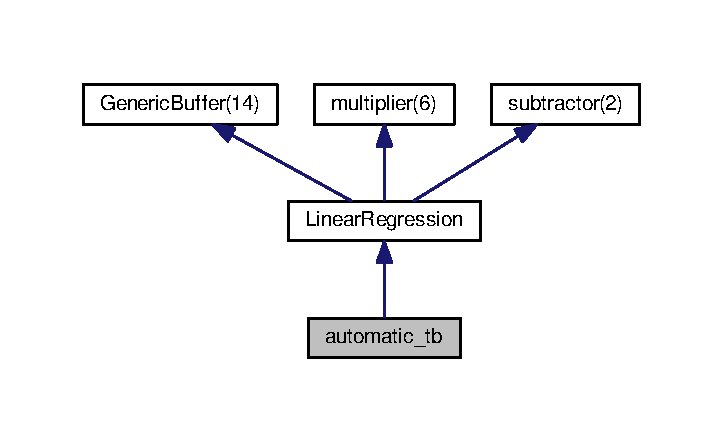
\includegraphics[width=258pt]{classautomatic__tb__inherit__graph}
\end{center}
\end{figure}


Diagramma di collaborazione per automatic\+\_\+tb\+:\nopagebreak
\begin{figure}[H]
\begin{center}
\leavevmode
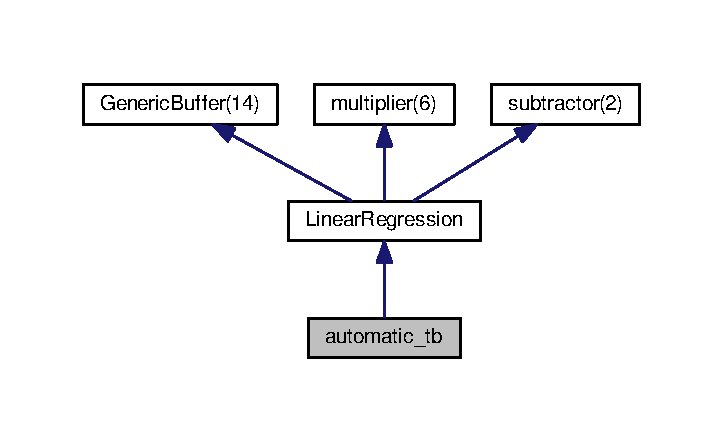
\includegraphics[width=258pt]{classautomatic__tb__coll__graph}
\end{center}
\end{figure}
\subsection*{Entities}
\begin{DoxyCompactItemize}
\item 
\hyperlink{classautomatic__tb_1_1behavioral}{behavioral} architecture
\end{DoxyCompactItemize}
\subsection*{Libraries}
 \begin{DoxyCompactItemize}
\item 
\hyperlink{classautomatic__tb_a0a6af6eef40212dbaf130d57ce711256}{ieee} 
\end{DoxyCompactItemize}
\subsection*{Use Clauses}
 \begin{DoxyCompactItemize}
\item 
\hyperlink{classautomatic__tb_acd03516902501cd1c7296a98e22c6fcb}{std\+\_\+logic\+\_\+1164}   
\item 
\hyperlink{classautomatic__tb_a2edc34402b573437d5f25fa90ba4013e}{numeric\+\_\+std}   
\item 
\hyperlink{classautomatic__tb_aa8c4e25998323a84db5b1fa701b92fcb}{textio}   
\item 
\hyperlink{classautomatic__tb_abc7d7fc2675847e1d861e3fda2b1990c}{std\+\_\+logic\+\_\+textio}   
\end{DoxyCompactItemize}


\subsection{Documentazione dei membri dato}
\hypertarget{classautomatic__tb_a0a6af6eef40212dbaf130d57ce711256}{\index{automatic\+\_\+tb@{automatic\+\_\+tb}!ieee@{ieee}}
\index{ieee@{ieee}!automatic\+\_\+tb@{automatic\+\_\+tb}}
\subsubsection[{ieee}]{\setlength{\rightskip}{0pt plus 5cm}{\bf ieee}\hspace{0.3cm}{\ttfamily [Library]}}}\label{classautomatic__tb_a0a6af6eef40212dbaf130d57ce711256}
\hypertarget{classautomatic__tb_a2edc34402b573437d5f25fa90ba4013e}{\index{automatic\+\_\+tb@{automatic\+\_\+tb}!numeric\+\_\+std@{numeric\+\_\+std}}
\index{numeric\+\_\+std@{numeric\+\_\+std}!automatic\+\_\+tb@{automatic\+\_\+tb}}
\subsubsection[{numeric\+\_\+std}]{\setlength{\rightskip}{0pt plus 5cm}{\bf numeric\+\_\+std}\hspace{0.3cm}{\ttfamily [Package]}}}\label{classautomatic__tb_a2edc34402b573437d5f25fa90ba4013e}
\hypertarget{classautomatic__tb_acd03516902501cd1c7296a98e22c6fcb}{\index{automatic\+\_\+tb@{automatic\+\_\+tb}!std\+\_\+logic\+\_\+1164@{std\+\_\+logic\+\_\+1164}}
\index{std\+\_\+logic\+\_\+1164@{std\+\_\+logic\+\_\+1164}!automatic\+\_\+tb@{automatic\+\_\+tb}}
\subsubsection[{std\+\_\+logic\+\_\+1164}]{\setlength{\rightskip}{0pt plus 5cm}{\bf std\+\_\+logic\+\_\+1164}\hspace{0.3cm}{\ttfamily [Package]}}}\label{classautomatic__tb_acd03516902501cd1c7296a98e22c6fcb}
\hypertarget{classautomatic__tb_abc7d7fc2675847e1d861e3fda2b1990c}{\index{automatic\+\_\+tb@{automatic\+\_\+tb}!std\+\_\+logic\+\_\+textio@{std\+\_\+logic\+\_\+textio}}
\index{std\+\_\+logic\+\_\+textio@{std\+\_\+logic\+\_\+textio}!automatic\+\_\+tb@{automatic\+\_\+tb}}
\subsubsection[{std\+\_\+logic\+\_\+textio}]{\setlength{\rightskip}{0pt plus 5cm}{\bf std\+\_\+logic\+\_\+textio}\hspace{0.3cm}{\ttfamily [Package]}}}\label{classautomatic__tb_abc7d7fc2675847e1d861e3fda2b1990c}
\hypertarget{classautomatic__tb_aa8c4e25998323a84db5b1fa701b92fcb}{\index{automatic\+\_\+tb@{automatic\+\_\+tb}!textio@{textio}}
\index{textio@{textio}!automatic\+\_\+tb@{automatic\+\_\+tb}}
\subsubsection[{textio}]{\setlength{\rightskip}{0pt plus 5cm}{\bf textio}\hspace{0.3cm}{\ttfamily [Package]}}}\label{classautomatic__tb_aa8c4e25998323a84db5b1fa701b92fcb}


La documentazione per questa classe è stata generata a partire dal seguente file\+:\begin{DoxyCompactItemize}
\item 
Src/testbench/\hyperlink{automatic__tb_8vhd}{automatic\+\_\+tb.\+vhd}\end{DoxyCompactItemize}

\hypertarget{class_generic_buffer_1_1_behavioral}{\section{Behavioral Architecture Reference}
\label{class_generic_buffer_1_1_behavioral}\index{Behavioral@{Behavioral}}
}


Implementazione behavioral di \hyperlink{class_generic_buffer}{Generic\+Buffer}.  


\subsection*{Processes}
 \begin{DoxyCompactItemize}
\item 
\hyperlink{group___generic_buffer_ga2ee480e118ca2b3fccf26139a66e84ad}{P\+R\+O\+C\+E\+S\+S\+\_\+0}{\bfseries  ( {\bfseries {\bfseries \hyperlink{group___generic_buffer_gadfc2d5e995e9c6876b2e55bf6a5c4071}{clock}} \textcolor{vhdlchar}{ }} , {\bfseries {\bfseries \hyperlink{group___generic_buffer_ga446ea52ed8c4a84181a47d9165ce41a5}{reset\+\_\+n}} \textcolor{vhdlchar}{ }} , {\bfseries {\bfseries \hyperlink{group___generic_buffer_gaba761f7740d0b6257a0e283b3734ddbf}{load}} \textcolor{vhdlchar}{ }} , {\bfseries {\bfseries \hyperlink{group___generic_buffer_ga597910698848749da5951285c85fa4f9}{data\+\_\+in}} \textcolor{vhdlchar}{ }} )}
\end{DoxyCompactItemize}
\subsection*{Signals}
 \begin{DoxyCompactItemize}
\item 
\hyperlink{group___generic_buffer_gab94e66105790803865249c33633e359f}{tmp} {\bfseries \textcolor{vhdlchar}{std\+\_\+logic\+\_\+vector}\textcolor{vhdlchar}{ }\textcolor{vhdlchar}{(}\textcolor{vhdlchar}{ }\textcolor{vhdlchar}{ }\textcolor{vhdlchar}{ }\textcolor{vhdlchar}{ }{\bfseries \hyperlink{group___generic_buffer_gae47d961480346c1d82439a66505e6e7d}{width}} \textcolor{vhdlchar}{-\/}\textcolor{vhdlchar}{ } \textcolor{vhdldigit}{1} \textcolor{vhdlchar}{ }\textcolor{vhdlchar}{downto}\textcolor{vhdlchar}{ }\textcolor{vhdlchar}{ } \textcolor{vhdldigit}{0} \textcolor{vhdlchar}{ }\textcolor{vhdlchar}{)}\textcolor{vhdlchar}{ }\textcolor{vhdlchar}{ }\textcolor{vhdlchar}{ }\textcolor{vhdlchar}{\+:}\textcolor{vhdlchar}{=}\textcolor{vhdlchar}{ }\textcolor{vhdlchar}{(}\textcolor{vhdlchar}{ }\textcolor{vhdlchar}{ }\textcolor{vhdlchar}{others}\textcolor{vhdlchar}{ }\textcolor{vhdlchar}{ }\textcolor{vhdlchar}{=}\textcolor{vhdlchar}{ }\textcolor{vhdlchar}{$>$}\textcolor{vhdlchar}{ }\textcolor{vhdlchar}{'}\textcolor{vhdlchar}{ } \textcolor{vhdldigit}{0} \textcolor{vhdlchar}{ }\textcolor{vhdlchar}{'}\textcolor{vhdlchar}{ }\textcolor{vhdlchar}{)}\textcolor{vhdlchar}{ }} 
\end{DoxyCompactItemize}


\subsection{Descrizione dettagliata}
Implementazione behavioral di \hyperlink{class_generic_buffer}{Generic\+Buffer}. 

La documentazione per questa classe è stata generata a partire dal seguente file\+:\begin{DoxyCompactItemize}
\item 
Src/\hyperlink{_generic_buffer_8vhd}{Generic\+Buffer.\+vhd}\end{DoxyCompactItemize}

\hypertarget{classautomatic__tb_1_1behavioral}{\section{behavioral Architecture Reference}
\label{classautomatic__tb_1_1behavioral}\index{behavioral@{behavioral}}
}
\subsection*{Processes}
 \begin{DoxyCompactItemize}
\item 
\hyperlink{classautomatic__tb_1_1behavioral_ac0731c1f0a226305f2a590b4044cdccb}{clock\+\_\+process}{\bfseries  (  )}
\item 
\hyperlink{classautomatic__tb_1_1behavioral_ad2efa6785cff833c341e27596b21aeb5}{stim\+\_\+proc}{\bfseries  (  )}
\end{DoxyCompactItemize}
\subsection*{Components}
 \begin{DoxyCompactItemize}
\item 
\hyperlink{classautomatic__tb_1_1behavioral_a899499ba78b32b936cd0914831a72c95}{Linear\+Regression}  {\bfseries }  
\end{DoxyCompactItemize}
\subsection*{Instantiations}
 \begin{DoxyCompactItemize}
\item 
\hyperlink{classautomatic__tb_1_1behavioral_a1619316ad715601eb5d3559db829ac05}{uut}  {\bfseries Linear\+Regression}   
\end{DoxyCompactItemize}


\subsection{Documentazione delle funzioni membro}
\hypertarget{classautomatic__tb_1_1behavioral_ac0731c1f0a226305f2a590b4044cdccb}{\index{automatic\+\_\+tb\+::behavioral@{automatic\+\_\+tb\+::behavioral}!clock\+\_\+process@{clock\+\_\+process}}
\index{clock\+\_\+process@{clock\+\_\+process}!automatic\+\_\+tb\+::behavioral@{automatic\+\_\+tb\+::behavioral}}
\subsubsection[{clock\+\_\+process}]{\setlength{\rightskip}{0pt plus 5cm} {\bfseries \textcolor{vhdlchar}{ }} clock\+\_\+process ( ) \hspace{0.3cm}{\ttfamily [Process]}}}\label{classautomatic__tb_1_1behavioral_ac0731c1f0a226305f2a590b4044cdccb}
\hypertarget{classautomatic__tb_1_1behavioral_ad2efa6785cff833c341e27596b21aeb5}{\index{automatic\+\_\+tb\+::behavioral@{automatic\+\_\+tb\+::behavioral}!stim\+\_\+proc@{stim\+\_\+proc}}
\index{stim\+\_\+proc@{stim\+\_\+proc}!automatic\+\_\+tb\+::behavioral@{automatic\+\_\+tb\+::behavioral}}
\subsubsection[{stim\+\_\+proc}]{\setlength{\rightskip}{0pt plus 5cm}stim\+\_\+proc (
\begin{DoxyParamCaption}
{}
\end{DoxyParamCaption}
)}}\label{classautomatic__tb_1_1behavioral_ad2efa6785cff833c341e27596b21aeb5}


\subsection{Documentazione dei membri dato}
\hypertarget{classautomatic__tb_1_1behavioral_a899499ba78b32b936cd0914831a72c95}{\index{automatic\+\_\+tb\+::behavioral@{automatic\+\_\+tb\+::behavioral}!Linear\+Regression@{Linear\+Regression}}
\index{Linear\+Regression@{Linear\+Regression}!automatic\+\_\+tb\+::behavioral@{automatic\+\_\+tb\+::behavioral}}
\subsubsection[{Linear\+Regression}]{\setlength{\rightskip}{0pt plus 5cm}{\bf Linear\+Regression} {\bfseries \textcolor{vhdlchar}{ }} \hspace{0.3cm}{\ttfamily [Component]}}}\label{classautomatic__tb_1_1behavioral_a899499ba78b32b936cd0914831a72c95}
\hypertarget{classautomatic__tb_1_1behavioral_a1619316ad715601eb5d3559db829ac05}{\index{automatic\+\_\+tb\+::behavioral@{automatic\+\_\+tb\+::behavioral}!uut@{uut}}
\index{uut@{uut}!automatic\+\_\+tb\+::behavioral@{automatic\+\_\+tb\+::behavioral}}
\subsubsection[{uut}]{\setlength{\rightskip}{0pt plus 5cm}{\bf uut} {\bfseries \textcolor{vhdlchar}{Linear\+Regression}\textcolor{vhdlchar}{ }} \hspace{0.3cm}{\ttfamily [Instantiation]}}}\label{classautomatic__tb_1_1behavioral_a1619316ad715601eb5d3559db829ac05}


La documentazione per questa classe è stata generata a partire dal seguente file\+:\begin{DoxyCompactItemize}
\item 
Src/testbench/\hyperlink{automatic__tb_8vhd}{automatic\+\_\+tb.\+vhd}\end{DoxyCompactItemize}

\hypertarget{classtb___linear_regression_1_1_behavioral}{}\section{Behavioral Architecture Reference}
\label{classtb___linear_regression_1_1_behavioral}\index{Behavioral@{Behavioral}}
\subsection*{Processes}
 \begin{DoxyCompactItemize}
\item 
\hyperlink{classtb___linear_regression_1_1_behavioral_ac0731c1f0a226305f2a590b4044cdccb}{clock\+\_\+process}{\bfseries  (  )}
\item 
\hyperlink{classtb___linear_regression_1_1_behavioral_ad2efa6785cff833c341e27596b21aeb5}{stim\+\_\+proc}{\bfseries  (  )}
\end{DoxyCompactItemize}
\subsection*{Components}
 \begin{DoxyCompactItemize}
\item 
\hyperlink{classtb___linear_regression_1_1_behavioral_a899499ba78b32b936cd0914831a72c95}{Linear\+Regression}  {\bfseries }  
\end{DoxyCompactItemize}
\subsection*{Instantiations}
 \begin{DoxyCompactItemize}
\item 
\hyperlink{classtb___linear_regression_1_1_behavioral_a1619316ad715601eb5d3559db829ac05}{uut}  {\bfseries Linear\+Regression}   
\end{DoxyCompactItemize}


\subsection{Documentazione delle funzioni membro}
\index{tb\+\_\+\+Linear\+Regression\+::\+Behavioral@{tb\+\_\+\+Linear\+Regression\+::\+Behavioral}!clock\+\_\+process@{clock\+\_\+process}}
\index{clock\+\_\+process@{clock\+\_\+process}!tb\+\_\+\+Linear\+Regression\+::\+Behavioral@{tb\+\_\+\+Linear\+Regression\+::\+Behavioral}}
\subsubsection[{\texorpdfstring{clock\+\_\+process}{clock_process}}]{\setlength{\rightskip}{0pt plus 5cm} {\bfseries \textcolor{vhdlchar}{ }} clock\+\_\+process ( ) \hspace{0.3cm}{\ttfamily [Process]}}\hypertarget{classtb___linear_regression_1_1_behavioral_ac0731c1f0a226305f2a590b4044cdccb}{}\label{classtb___linear_regression_1_1_behavioral_ac0731c1f0a226305f2a590b4044cdccb}
\index{tb\+\_\+\+Linear\+Regression\+::\+Behavioral@{tb\+\_\+\+Linear\+Regression\+::\+Behavioral}!stim\+\_\+proc@{stim\+\_\+proc}}
\index{stim\+\_\+proc@{stim\+\_\+proc}!tb\+\_\+\+Linear\+Regression\+::\+Behavioral@{tb\+\_\+\+Linear\+Regression\+::\+Behavioral}}
\subsubsection[{\texorpdfstring{stim\+\_\+proc}{stim_proc}}]{\setlength{\rightskip}{0pt plus 5cm}stim\+\_\+proc (
\begin{DoxyParamCaption}
{}
\end{DoxyParamCaption}
)}\hypertarget{classtb___linear_regression_1_1_behavioral_ad2efa6785cff833c341e27596b21aeb5}{}\label{classtb___linear_regression_1_1_behavioral_ad2efa6785cff833c341e27596b21aeb5}


\subsection{Documentazione dei membri dato}
\index{tb\+\_\+\+Linear\+Regression\+::\+Behavioral@{tb\+\_\+\+Linear\+Regression\+::\+Behavioral}!Linear\+Regression@{Linear\+Regression}}
\index{Linear\+Regression@{Linear\+Regression}!tb\+\_\+\+Linear\+Regression\+::\+Behavioral@{tb\+\_\+\+Linear\+Regression\+::\+Behavioral}}
\subsubsection[{\texorpdfstring{Linear\+Regression}{LinearRegression}}]{\setlength{\rightskip}{0pt plus 5cm}{\bf Linear\+Regression} {\bfseries \textcolor{vhdlchar}{ }} \hspace{0.3cm}{\ttfamily [Component]}}\hypertarget{classtb___linear_regression_1_1_behavioral_a899499ba78b32b936cd0914831a72c95}{}\label{classtb___linear_regression_1_1_behavioral_a899499ba78b32b936cd0914831a72c95}
\index{tb\+\_\+\+Linear\+Regression\+::\+Behavioral@{tb\+\_\+\+Linear\+Regression\+::\+Behavioral}!uut@{uut}}
\index{uut@{uut}!tb\+\_\+\+Linear\+Regression\+::\+Behavioral@{tb\+\_\+\+Linear\+Regression\+::\+Behavioral}}
\subsubsection[{\texorpdfstring{uut}{uut}}]{\setlength{\rightskip}{0pt plus 5cm}{\bf uut} {\bfseries \textcolor{vhdlchar}{Linear\+Regression}\textcolor{vhdlchar}{ }} \hspace{0.3cm}{\ttfamily [Instantiation]}}\hypertarget{classtb___linear_regression_1_1_behavioral_a1619316ad715601eb5d3559db829ac05}{}\label{classtb___linear_regression_1_1_behavioral_a1619316ad715601eb5d3559db829ac05}


La documentazione per questa classe è stata generata a partire dal seguente file\+:\begin{DoxyCompactItemize}
\item 
Src/testbench/\hyperlink{tb___linear_regression_8vhd}{tb\+\_\+\+Linear\+Regression.\+vhd}\end{DoxyCompactItemize}

\hypertarget{class_generic_buffer}{\section{Generic\+Buffer Entity Reference}
\label{class_generic_buffer}\index{Generic\+Buffer@{Generic\+Buffer}}
}


Registro di dimensione generica.  




Diagramma delle classi per Generic\+Buffer\nopagebreak
\begin{figure}[H]
\begin{center}
\leavevmode
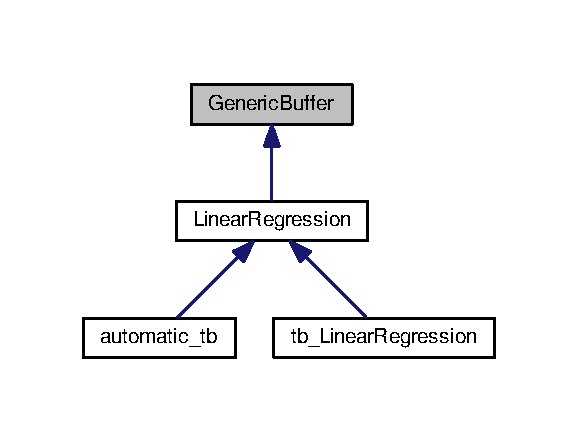
\includegraphics[width=278pt]{class_generic_buffer__inherit__graph}
\end{center}
\end{figure}
\subsection*{Entities}
\begin{DoxyCompactItemize}
\item 
\hyperlink{class_generic_buffer_1_1_behavioral}{Behavioral} architecture
\begin{DoxyCompactList}\small\item\em Implementazione behavioral di \hyperlink{class_generic_buffer}{Generic\+Buffer}. \end{DoxyCompactList}\end{DoxyCompactItemize}
\subsection*{Libraries}
 \begin{DoxyCompactItemize}
\item 
\hyperlink{group___generic_buffer_ga0a6af6eef40212dbaf130d57ce711256}{ieee} 
\end{DoxyCompactItemize}
\subsection*{Use Clauses}
 \begin{DoxyCompactItemize}
\item 
\hyperlink{group___generic_buffer_gacd03516902501cd1c7296a98e22c6fcb}{std\+\_\+logic\+\_\+1164}   
\end{DoxyCompactItemize}
\subsection*{Generics}
 \begin{DoxyCompactItemize}
\item 
\hyperlink{group___generic_buffer_gae47d961480346c1d82439a66505e6e7d}{width} {\bfseries {\bfseries \textcolor{vhdlchar}{natural}\textcolor{vhdlchar}{ }\textcolor{vhdlchar}{ }\textcolor{vhdlchar}{\+:}\textcolor{vhdlchar}{=}\textcolor{vhdlchar}{ }\textcolor{vhdlchar}{ } \textcolor{vhdldigit}{8} \textcolor{vhdlchar}{ }}}
\begin{DoxyCompactList}\small\item\em numero di bit del registro \end{DoxyCompactList}\item 
\hyperlink{group___generic_buffer_ga9079dbf8b7827a9cf522497d56994375}{edge} {\bfseries {\bfseries \textcolor{vhdlchar}{std\+\_\+logic}\textcolor{vhdlchar}{ }\textcolor{vhdlchar}{ }\textcolor{vhdlchar}{\+:}\textcolor{vhdlchar}{=}\textcolor{vhdlchar}{ }\textcolor{vhdlchar}{ }\textcolor{vhdlchar}{'}\textcolor{vhdlchar}{ } \textcolor{vhdldigit}{1} \textcolor{vhdlchar}{ }\textcolor{vhdlchar}{'}\textcolor{vhdlchar}{ }}}
\begin{DoxyCompactList}\small\item\em fronte di attivo del clock\+:
\begin{DoxyItemize}
\item '1'\+: fronte di salita
\item '0'\+: fronte di discesa 
\end{DoxyItemize}\end{DoxyCompactList}\end{DoxyCompactItemize}
\subsection*{Ports}
 \begin{DoxyCompactItemize}
\item 
\hyperlink{group___generic_buffer_gadfc2d5e995e9c6876b2e55bf6a5c4071}{clock}  {\bfseries {\bfseries \textcolor{vhdlchar}{in}\textcolor{vhdlchar}{ }}} {\bfseries \textcolor{vhdlchar}{std\+\_\+logic}\textcolor{vhdlchar}{ }} 
\begin{DoxyCompactList}\small\item\em segnale di clock \end{DoxyCompactList}\item 
\hyperlink{group___generic_buffer_ga446ea52ed8c4a84181a47d9165ce41a5}{reset\+\_\+n}  {\bfseries {\bfseries \textcolor{vhdlchar}{in}\textcolor{vhdlchar}{ }}} {\bfseries \textcolor{vhdlchar}{std\+\_\+logic}\textcolor{vhdlchar}{ }} 
\begin{DoxyCompactList}\small\item\em reset asincrono, attivo basso \end{DoxyCompactList}\item 
\hyperlink{group___generic_buffer_gaba761f7740d0b6257a0e283b3734ddbf}{load}  {\bfseries {\bfseries \textcolor{vhdlchar}{in}\textcolor{vhdlchar}{ }}} {\bfseries \textcolor{vhdlchar}{std\+\_\+logic}\textcolor{vhdlchar}{ }} 
\begin{DoxyCompactList}\small\item\em segnale di load, quando '1' l'uscita (data\+\_\+out) segue l'ingresso (data\+\_\+in) \end{DoxyCompactList}\item 
\hyperlink{group___generic_buffer_ga597910698848749da5951285c85fa4f9}{data\+\_\+in}  {\bfseries {\bfseries \textcolor{vhdlchar}{in}\textcolor{vhdlchar}{ }}} {\bfseries \textcolor{vhdlchar}{std\+\_\+logic\+\_\+vector}\textcolor{vhdlchar}{ }\textcolor{vhdlchar}{(}\textcolor{vhdlchar}{ }\textcolor{vhdlchar}{ }\textcolor{vhdlchar}{ }\textcolor{vhdlchar}{ }{\bfseries \hyperlink{group___generic_buffer_gae47d961480346c1d82439a66505e6e7d}{width}} \textcolor{vhdlchar}{-\/}\textcolor{vhdlchar}{ } \textcolor{vhdldigit}{1} \textcolor{vhdlchar}{ }\textcolor{vhdlchar}{downto}\textcolor{vhdlchar}{ }\textcolor{vhdlchar}{ } \textcolor{vhdldigit}{0} \textcolor{vhdlchar}{ }\textcolor{vhdlchar}{)}\textcolor{vhdlchar}{ }} 
\begin{DoxyCompactList}\small\item\em ingresso del registro \end{DoxyCompactList}\item 
\hyperlink{group___generic_buffer_ga0bf60a72cb11ffe1945b82ce0bb86a57}{data\+\_\+out}  {\bfseries {\bfseries \textcolor{vhdlchar}{out}\textcolor{vhdlchar}{ }}} {\bfseries \textcolor{vhdlchar}{std\+\_\+logic\+\_\+vector}\textcolor{vhdlchar}{ }\textcolor{vhdlchar}{(}\textcolor{vhdlchar}{ }\textcolor{vhdlchar}{ }\textcolor{vhdlchar}{ }\textcolor{vhdlchar}{ }{\bfseries \hyperlink{group___generic_buffer_gae47d961480346c1d82439a66505e6e7d}{width}} \textcolor{vhdlchar}{-\/}\textcolor{vhdlchar}{ } \textcolor{vhdldigit}{1} \textcolor{vhdlchar}{ }\textcolor{vhdlchar}{downto}\textcolor{vhdlchar}{ }\textcolor{vhdlchar}{ } \textcolor{vhdldigit}{0} \textcolor{vhdlchar}{ }\textcolor{vhdlchar}{)}\textcolor{vhdlchar}{ }} 
\begin{DoxyCompactList}\small\item\em uscita del registro \end{DoxyCompactList}\end{DoxyCompactItemize}


\subsection{Descrizione dettagliata}
Registro di dimensione generica. 

La documentazione per questa classe è stata generata a partire dal seguente file\+:\begin{DoxyCompactItemize}
\item 
Src/\hyperlink{_generic_buffer_8vhd}{Generic\+Buffer.\+vhd}\end{DoxyCompactItemize}

\hypertarget{class_linear_regression}{}\section{Linear\+Regression Entity Reference}
\label{class_linear_regression}\index{Linear\+Regression@{Linear\+Regression}}


Diagramma delle classi per Linear\+Regression\nopagebreak
\begin{figure}[H]
\begin{center}
\leavevmode
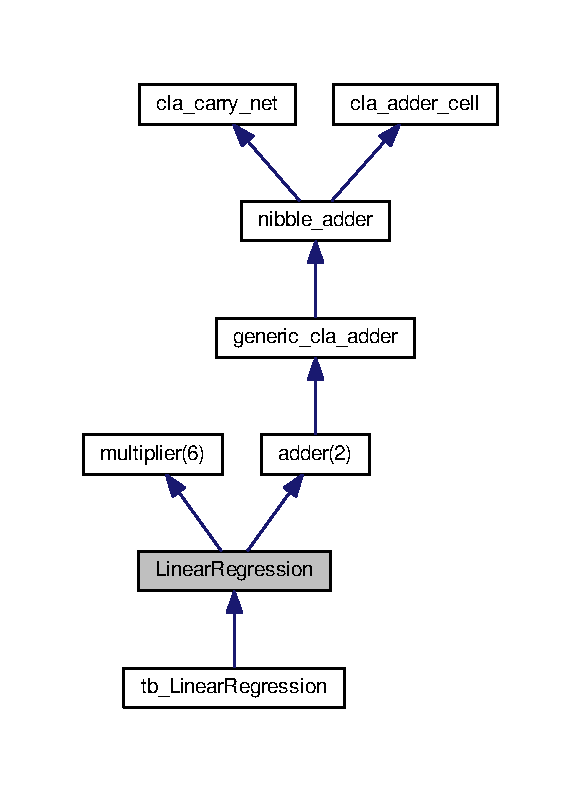
\includegraphics[width=279pt]{class_linear_regression__inherit__graph}
\end{center}
\end{figure}


Diagramma di collaborazione per Linear\+Regression\+:\nopagebreak
\begin{figure}[H]
\begin{center}
\leavevmode
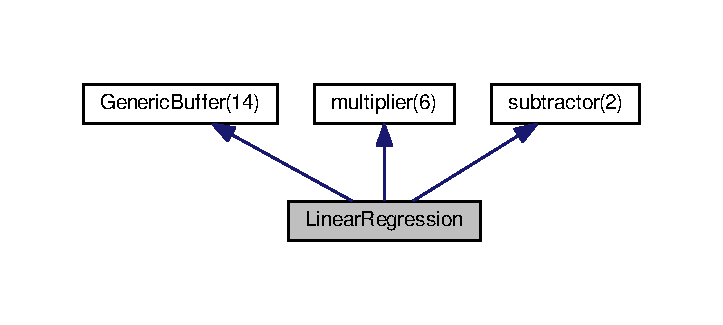
\includegraphics[width=279pt]{class_linear_regression__coll__graph}
\end{center}
\end{figure}
\subsection*{Entities}
\begin{DoxyCompactItemize}
\item 
\hyperlink{class_linear_regression_1_1_structural}{Structural} architecture
\end{DoxyCompactItemize}
\subsection*{Libraries}
 \begin{DoxyCompactItemize}
\item 
\hyperlink{group___linear_regression_gae4f03c286607f3181e16b9aa12d0c6d4}{I\+E\+EE} 
\end{DoxyCompactItemize}
\subsection*{Use Clauses}
 \begin{DoxyCompactItemize}
\item 
\hyperlink{group___linear_regression_gaa4b2b25246a821511120e3149b003563}{S\+T\+D\+\_\+\+L\+O\+G\+I\+C\+\_\+1164}   
\item 
\hyperlink{group___linear_regression_gae00f3f04545af57582ff10609eee23e2}{N\+U\+M\+E\+R\+I\+C\+\_\+\+S\+TD}   
\end{DoxyCompactItemize}
\subsection*{Ports}
 \begin{DoxyCompactItemize}
\item 
\hyperlink{group___linear_regression_ga6b9afe9c48db695b7336519281c099a8}{prim}  {\bfseries {\bfseries \textcolor{vhdlchar}{in}\textcolor{vhdlchar}{ }}} {\bfseries \textcolor{vhdlchar}{S\+T\+D\+\_\+\+L\+O\+G\+I\+C\+\_\+\+V\+E\+C\+T\+OR}\textcolor{vhdlchar}{ }\textcolor{vhdlchar}{(}\textcolor{vhdlchar}{ }\textcolor{vhdlchar}{ } \textcolor{vhdldigit}{4} \textcolor{vhdlchar}{ }\textcolor{vhdlchar}{downto}\textcolor{vhdlchar}{ }\textcolor{vhdlchar}{ } \textcolor{vhdldigit}{0} \textcolor{vhdlchar}{ }\textcolor{vhdlchar}{)}\textcolor{vhdlchar}{ }} 
\begin{DoxyCompactList}\small\item\em costante in input, 5 bit di parte intera e 0 decimale (m.\+n = 4.\+0) \end{DoxyCompactList}\item 
\hyperlink{group___linear_regression_ga4c98819455589b84c5e250a97e9bdfa1}{Sum2}  {\bfseries {\bfseries \textcolor{vhdlchar}{in}\textcolor{vhdlchar}{ }}} {\bfseries \textcolor{vhdlchar}{S\+T\+D\+\_\+\+L\+O\+G\+I\+C\+\_\+\+V\+E\+C\+T\+OR}\textcolor{vhdlchar}{ }\textcolor{vhdlchar}{(}\textcolor{vhdlchar}{ }\textcolor{vhdlchar}{ } \textcolor{vhdldigit}{23} \textcolor{vhdlchar}{ }\textcolor{vhdlchar}{downto}\textcolor{vhdlchar}{ }\textcolor{vhdlchar}{ } \textcolor{vhdldigit}{0} \textcolor{vhdlchar}{ }\textcolor{vhdlchar}{)}\textcolor{vhdlchar}{ }} 
\begin{DoxyCompactList}\small\item\em segnale in input, 3 bit di parte intera e 21 decimale (m.\+n = 2.\+21) \end{DoxyCompactList}\item 
\hyperlink{group___linear_regression_gab6685be06ffd9f2425d01307287a4454}{B}  {\bfseries {\bfseries \textcolor{vhdlchar}{in}\textcolor{vhdlchar}{ }}} {\bfseries \textcolor{vhdlchar}{S\+T\+D\+\_\+\+L\+O\+G\+I\+C\+\_\+\+V\+E\+C\+T\+OR}\textcolor{vhdlchar}{ }\textcolor{vhdlchar}{(}\textcolor{vhdlchar}{ }\textcolor{vhdlchar}{ } \textcolor{vhdldigit}{23} \textcolor{vhdlchar}{ }\textcolor{vhdlchar}{downto}\textcolor{vhdlchar}{ }\textcolor{vhdlchar}{ } \textcolor{vhdldigit}{0} \textcolor{vhdlchar}{ }\textcolor{vhdlchar}{)}\textcolor{vhdlchar}{ }} 
\begin{DoxyCompactList}\small\item\em segnale in input, 3 bit di parte intera e 21 decimale (m.\+n = 2.\+21) \end{DoxyCompactList}\item 
\hyperlink{group___linear_regression_ga43a9a0da4f44006af5631ed5ee8ad924}{Sum1}  {\bfseries {\bfseries \textcolor{vhdlchar}{in}\textcolor{vhdlchar}{ }}} {\bfseries \textcolor{vhdlchar}{S\+T\+D\+\_\+\+L\+O\+G\+I\+C\+\_\+\+V\+E\+C\+T\+OR}\textcolor{vhdlchar}{ }\textcolor{vhdlchar}{(}\textcolor{vhdlchar}{ }\textcolor{vhdlchar}{ } \textcolor{vhdldigit}{23} \textcolor{vhdlchar}{ }\textcolor{vhdlchar}{downto}\textcolor{vhdlchar}{ }\textcolor{vhdlchar}{ } \textcolor{vhdldigit}{0} \textcolor{vhdlchar}{ }\textcolor{vhdlchar}{)}\textcolor{vhdlchar}{ }} 
\begin{DoxyCompactList}\small\item\em segnale in input, 8 bit di parte intera e 16 decimale (m.\+n = 7.\+16) \end{DoxyCompactList}\item 
\hyperlink{group___linear_regression_ga17058a6bcb609074c49be51d09202870}{C}  {\bfseries {\bfseries \textcolor{vhdlchar}{in}\textcolor{vhdlchar}{ }}} {\bfseries \textcolor{vhdlchar}{S\+T\+D\+\_\+\+L\+O\+G\+I\+C\+\_\+\+V\+E\+C\+T\+OR}\textcolor{vhdlchar}{ }\textcolor{vhdlchar}{(}\textcolor{vhdlchar}{ }\textcolor{vhdlchar}{ } \textcolor{vhdldigit}{23} \textcolor{vhdlchar}{ }\textcolor{vhdlchar}{downto}\textcolor{vhdlchar}{ }\textcolor{vhdlchar}{ } \textcolor{vhdldigit}{0} \textcolor{vhdlchar}{ }\textcolor{vhdlchar}{)}\textcolor{vhdlchar}{ }} 
\begin{DoxyCompactList}\small\item\em segnale in input, msb di peso -\/10 (m.\+n = -\/10.\+33) \end{DoxyCompactList}\item 
\hyperlink{group___linear_regression_gae1ad6503d157f6c26abdce1131d31ec2}{A}  {\bfseries {\bfseries \textcolor{vhdlchar}{in}\textcolor{vhdlchar}{ }}} {\bfseries \textcolor{vhdlchar}{S\+T\+D\+\_\+\+L\+O\+G\+I\+C\+\_\+\+V\+E\+C\+T\+OR}\textcolor{vhdlchar}{ }\textcolor{vhdlchar}{(}\textcolor{vhdlchar}{ }\textcolor{vhdlchar}{ } \textcolor{vhdldigit}{23} \textcolor{vhdlchar}{ }\textcolor{vhdlchar}{downto}\textcolor{vhdlchar}{ }\textcolor{vhdlchar}{ } \textcolor{vhdldigit}{0} \textcolor{vhdlchar}{ }\textcolor{vhdlchar}{)}\textcolor{vhdlchar}{ }} 
\begin{DoxyCompactList}\small\item\em segnale in input, 16 bit di parte intera e 8 decimale (m.\+n = 15.\+8) \end{DoxyCompactList}\item 
\hyperlink{group___linear_regression_gad943f01112876248a4734aa3c3d2e3f2}{m}  {\bfseries {\bfseries \textcolor{vhdlchar}{out}\textcolor{vhdlchar}{ }}} {\bfseries \textcolor{vhdlchar}{S\+T\+D\+\_\+\+L\+O\+G\+I\+C\+\_\+\+V\+E\+C\+T\+OR}\textcolor{vhdlchar}{ }\textcolor{vhdlchar}{(}\textcolor{vhdlchar}{ }\textcolor{vhdlchar}{ } \textcolor{vhdldigit}{23} \textcolor{vhdlchar}{ }\textcolor{vhdlchar}{downto}\textcolor{vhdlchar}{ }\textcolor{vhdlchar}{ } \textcolor{vhdldigit}{0} \textcolor{vhdlchar}{ }\textcolor{vhdlchar}{)}\textcolor{vhdlchar}{ }} 
\begin{DoxyCompactList}\small\item\em segnale in output, 16 bit di parte intera e 8 decimale (m.\+n = 15.\+8) \end{DoxyCompactList}\item 
\hyperlink{group___linear_regression_gacec4f4b6d139d1ada088ca2d3d881418}{q}  {\bfseries {\bfseries \textcolor{vhdlchar}{out}\textcolor{vhdlchar}{ }}} {\bfseries \textcolor{vhdlchar}{S\+T\+D\+\_\+\+L\+O\+G\+I\+C\+\_\+\+V\+E\+C\+T\+OR}\textcolor{vhdlchar}{ }\textcolor{vhdlchar}{(}\textcolor{vhdlchar}{ }\textcolor{vhdlchar}{ } \textcolor{vhdldigit}{23} \textcolor{vhdlchar}{ }\textcolor{vhdlchar}{downto}\textcolor{vhdlchar}{ }\textcolor{vhdlchar}{ } \textcolor{vhdldigit}{0} \textcolor{vhdlchar}{ }\textcolor{vhdlchar}{)}\textcolor{vhdlchar}{ }} 
\begin{DoxyCompactList}\small\item\em segnaes in output, 8 bit di parte intera e 16 decimale (m.\+n = 7.\+16) \end{DoxyCompactList}\end{DoxyCompactItemize}


La documentazione per questa classe è stata generata a partire dal seguente file\+:\begin{DoxyCompactItemize}
\item 
Src/\hyperlink{_linear_regression_8vhd}{Linear\+Regression.\+vhd}\end{DoxyCompactItemize}

\hypertarget{classmultiplier}{}\section{multiplier Entity Reference}
\label{classmultiplier}\index{multiplier@{multiplier}}


Diagramma delle classi per multiplier\nopagebreak
\begin{figure}[H]
\begin{center}
\leavevmode
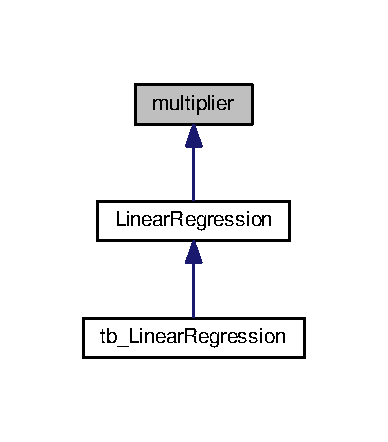
\includegraphics[width=278pt]{classmultiplier__inherit__graph}
\end{center}
\end{figure}
\subsection*{Entities}
\begin{DoxyCompactItemize}
\item 
\hyperlink{classmultiplier_1_1_structural}{Structural} architecture
\begin{DoxyCompactList}\small\item\em Per il prodotto viene utilizzato l\textquotesingle{}operatore $\ast$. La sintesi viene lasciata al particolare sintetizzatore. \end{DoxyCompactList}\end{DoxyCompactItemize}
\subsection*{Generics}
 \begin{DoxyCompactItemize}
\item 
\hyperlink{group___multiplier_ga4ede473cdc13e75fe66fbd548b62e432}{nbits1} {\bfseries {\bfseries \textcolor{vhdlchar}{natural}\textcolor{vhdlchar}{ }\textcolor{vhdlchar}{ }\textcolor{vhdlchar}{\+:}\textcolor{vhdlchar}{=}\textcolor{vhdlchar}{ }\textcolor{vhdlchar}{ } \textcolor{vhdldigit}{8} \textcolor{vhdlchar}{ }}}
\begin{DoxyCompactList}\small\item\em dimensione del primo fattore \end{DoxyCompactList}\item 
\hyperlink{group___multiplier_ga8b5bdaff4c3669528aaec95a07e17c2a}{nbits2} {\bfseries {\bfseries \textcolor{vhdlchar}{natural}\textcolor{vhdlchar}{ }\textcolor{vhdlchar}{ }\textcolor{vhdlchar}{\+:}\textcolor{vhdlchar}{=}\textcolor{vhdlchar}{ }\textcolor{vhdlchar}{ } \textcolor{vhdldigit}{8} \textcolor{vhdlchar}{ }}}
\begin{DoxyCompactList}\small\item\em dimensione del secondo fattore \end{DoxyCompactList}\end{DoxyCompactItemize}
\subsection*{Ports}
 \begin{DoxyCompactItemize}
\item 
\hyperlink{group___multiplier_gac728adecdbfe10213256c17c1b5c5128}{factor1}  {\bfseries {\bfseries \textcolor{vhdlchar}{in}\textcolor{vhdlchar}{ }}} {\bfseries \textcolor{vhdlchar}{S\+T\+D\+\_\+\+L\+O\+G\+I\+C\+\_\+\+V\+E\+C\+T\+OR}\textcolor{vhdlchar}{ }\textcolor{vhdlchar}{(}\textcolor{vhdlchar}{ }\textcolor{vhdlchar}{ }\textcolor{vhdlchar}{ }\textcolor{vhdlchar}{ }{\bfseries \hyperlink{group___multiplier_ga4ede473cdc13e75fe66fbd548b62e432}{nbits1}} \textcolor{vhdlchar}{-\/}\textcolor{vhdlchar}{ } \textcolor{vhdldigit}{1} \textcolor{vhdlchar}{ }\textcolor{vhdlchar}{downto}\textcolor{vhdlchar}{ }\textcolor{vhdlchar}{ } \textcolor{vhdldigit}{0} \textcolor{vhdlchar}{ }\textcolor{vhdlchar}{)}\textcolor{vhdlchar}{ }} 
\begin{DoxyCompactList}\small\item\em fattore 1 \end{DoxyCompactList}\item 
\hyperlink{group___multiplier_gac140852334303b430bbd49689cc689dd}{factor2}  {\bfseries {\bfseries \textcolor{vhdlchar}{in}\textcolor{vhdlchar}{ }}} {\bfseries \textcolor{vhdlchar}{S\+T\+D\+\_\+\+L\+O\+G\+I\+C\+\_\+\+V\+E\+C\+T\+OR}\textcolor{vhdlchar}{ }\textcolor{vhdlchar}{(}\textcolor{vhdlchar}{ }\textcolor{vhdlchar}{ }\textcolor{vhdlchar}{ }\textcolor{vhdlchar}{ }{\bfseries \hyperlink{group___multiplier_ga8b5bdaff4c3669528aaec95a07e17c2a}{nbits2}} \textcolor{vhdlchar}{-\/}\textcolor{vhdlchar}{ } \textcolor{vhdldigit}{1} \textcolor{vhdlchar}{ }\textcolor{vhdlchar}{downto}\textcolor{vhdlchar}{ }\textcolor{vhdlchar}{ } \textcolor{vhdldigit}{0} \textcolor{vhdlchar}{ }\textcolor{vhdlchar}{)}\textcolor{vhdlchar}{ }} 
\begin{DoxyCompactList}\small\item\em fattore 2 \end{DoxyCompactList}\item 
\hyperlink{group___multiplier_gaf168dc69ad77dc5791b5e0f99dcfb0a9}{prod}  {\bfseries {\bfseries \textcolor{vhdlchar}{out}\textcolor{vhdlchar}{ }}} {\bfseries \textcolor{vhdlchar}{S\+T\+D\+\_\+\+L\+O\+G\+I\+C\+\_\+\+V\+E\+C\+T\+OR}\textcolor{vhdlchar}{ }\textcolor{vhdlchar}{(}\textcolor{vhdlchar}{ }\textcolor{vhdlchar}{ }\textcolor{vhdlchar}{ }\textcolor{vhdlchar}{ }{\bfseries \hyperlink{group___multiplier_ga4ede473cdc13e75fe66fbd548b62e432}{nbits1}} \textcolor{vhdlchar}{+}\textcolor{vhdlchar}{ }\textcolor{vhdlchar}{ }\textcolor{vhdlchar}{ }{\bfseries \hyperlink{group___multiplier_ga8b5bdaff4c3669528aaec95a07e17c2a}{nbits2}} \textcolor{vhdlchar}{-\/}\textcolor{vhdlchar}{ } \textcolor{vhdldigit}{1} \textcolor{vhdlchar}{ }\textcolor{vhdlchar}{downto}\textcolor{vhdlchar}{ }\textcolor{vhdlchar}{ } \textcolor{vhdldigit}{0} \textcolor{vhdlchar}{ }\textcolor{vhdlchar}{)}\textcolor{vhdlchar}{ }} 
\begin{DoxyCompactList}\small\item\em prodotto dei due fattori \end{DoxyCompactList}\end{DoxyCompactItemize}


\subsection{Descrizione dettagliata}
Moltiplicatore a due fattori.

Il moltiplicatore permette di effettuare un prodotto di due fattori espressi su un certo numero di bit. I due fattori possono essere espressi anche su un numero di bit e rappresentazioni differenti tra loro. Se nbit1 è il numero di bit su cui viene espresso il fattore 1, e nbit2 è il numero di bit su cui viene espresso il fattore 2, allora l\textquotesingle{}uscita prod risulta essere espressa su nbit1+nbit2. ~\newline
 Ad esempio, se il fattore 1 è rappresentato con mx.\+nx (con mx il peso del bit più significativo della parte intera ed nx il peso del bit meno significativo della parte decimale) e il fattore 2 è rappresentato con my.\+ny, allora l\textquotesingle{}uscita sarà rappresentata in mx+my+1.nx+ny 

La documentazione per questa classe è stata generata a partire dal seguente file\+:\begin{DoxyCompactItemize}
\item 
Src/\hyperlink{multiplier_8vhd}{multiplier.\+vhd}\end{DoxyCompactItemize}

\hypertarget{classsubtractor_1_1structural}{}\section{structural Architecture Reference}
\label{classsubtractor_1_1structural}\index{structural@{structural}}


La documentazione per questa classe è stata generata a partire dal seguente file\+:\begin{DoxyCompactItemize}
\item 
Src/\hyperlink{subtractor_8vhd}{subtractor.\+vhd}\end{DoxyCompactItemize}

\hypertarget{class_linear_regression_1_1_structural}{}\section{Structural Architecture Reference}
\label{class_linear_regression_1_1_structural}\index{Structural@{Structural}}


8 

M\+U\+L\+T1, M\+U\+L\+T2, M\+U\+L\+T3, M\+U\+L\+T4, A\+D\+D5, A\+D\+D6, M\+U\+L\+T6 

Verificare che il troncamento post M\+U\+L\+T6 venga effettuato correttamente (7 bit in testa e 17 in coda) 

C=b\char`\"{}011000011101000101011010\char`\"{}~\newline
 Sum2=b\char`\"{}001010111100110111101111\char`\"{}~\newline
 B=b\char`\"{}001000110100010101100111\char`\"{}~\newline
 Sum1=b\char`\"{}001101001011110110010011\char`\"{}~\newline
 A=b\char`\"{}000111101111000111001010\char`\"{}  

mult2\+\_\+out=b\char`\"{}000001100000100100000111110011100100011000101001\char`\"{}~\newline
 P2= b\char`\"{}000010010000011111001110\char`\"{}~\newline
 mult4\+\_\+out=b\char`\"{}000101000010011011110110000000101010100010101110\char`\"{}~\newline
 P4= b\char`\"{}001010000100110111101100\char`\"{}~\newline
 add2\+\_\+out= b\char`\"{}001100010101010110111010\char`\"{}~\newline
 S6= b\char`\"{}000110001010101011011101\char`\"{}~\newline
 mult1\+\_\+out=b\char`\"{}00001101101100000101101010110\char`\"{}~\newline
 P3= b\char`\"{}011011011000001011010101\char`\"{}~\newline
 mult3\+\_\+out=b\char`\"{}000001110100010000110111011010011110010100100101\char`\"{}~\newline
 P1= b\char`\"{}110100010000110111011010\char`\"{}~\newline
 S5= b\char`\"{}001111101001000010101111\char`\"{}~\newline
 mult6\+\_\+out=b\char`\"{}000000101111101101010010001101101101111101100010\char`\"{}~\newline
 q =b\char`\"{}011111011010100100011011\char`\"{}  

mult2\+\_\+out=b\char`\"{}000001100000100100000111110011100100011000101001\char`\"{}~\newline
 P2= b\char`\"{}000010010000011111001110\char`\"{}~\newline
 mult4\+\_\+out=b\char`\"{}000101000010011011110110000000101010100010101110\char`\"{}~\newline
 P4= b\char`\"{}001010000100110111101100\char`\"{}~\newline
 add2\+\_\+out= b\char`\"{}001100010101010110111010\char`\"{}~\newline
 S6= b\char`\"{}000110001010101011011101\char`\"{}~\newline
 mult1\+\_\+out=b\char`\"{}00001101101100000101101010110\char`\"{}~\newline
 P3= b\char`\"{}011011011000001011010101\char`\"{}~\newline
 mult3\+\_\+out=b\char`\"{}000001110100010000110111011010011110010100100101\char`\"{}~\newline
 P1= b\char`\"{}110100010000110111011010\char`\"{}~\newline
 S5= b\char`\"{}001111101001000010101111\char`\"{}~\newline
 mult6\+\_\+out=b\char`\"{}000000101111101101010010001101101101111101100010\char`\"{}~\newline
 q =b\char`\"{}       011111011010100100011011\char`\"{}  

Superato   


\subsection*{Components}
 \begin{DoxyCompactItemize}
\item 
\hyperlink{group___linear_regression_ga3cf9cbfc3e637ae0660c32ceef50386f}{multiplier}  {\bfseries }  
\item 
\hyperlink{group___linear_regression_ga9d7a8a381439c61aea549e7a47ec7a6f}{adder}  {\bfseries }  
\end{DoxyCompactItemize}
\subsection*{Signals}
 \begin{DoxyCompactItemize}
\item 
\hyperlink{group___linear_regression_ga8e3ef6c468a1560f19de3430d956a75c}{mult1\+\_\+out} {\bfseries \textcolor{vhdlchar}{std\+\_\+logic\+\_\+vector}\textcolor{vhdlchar}{ }\textcolor{vhdlchar}{(}\textcolor{vhdlchar}{ }\textcolor{vhdlchar}{ } \textcolor{vhdldigit}{28} \textcolor{vhdlchar}{ }\textcolor{vhdlchar}{downto}\textcolor{vhdlchar}{ }\textcolor{vhdlchar}{ } \textcolor{vhdldigit}{0} \textcolor{vhdlchar}{ }\textcolor{vhdlchar}{)}\textcolor{vhdlchar}{ }\textcolor{vhdlchar}{ }\textcolor{vhdlchar}{ }\textcolor{vhdlchar}{\+:}\textcolor{vhdlchar}{=}\textcolor{vhdlchar}{ }\textcolor{vhdlchar}{(}\textcolor{vhdlchar}{ }\textcolor{vhdlchar}{ }\textcolor{vhdlchar}{others}\textcolor{vhdlchar}{ }\textcolor{vhdlchar}{ }\textcolor{vhdlchar}{=}\textcolor{vhdlchar}{ }\textcolor{vhdlchar}{$>$}\textcolor{vhdlchar}{ }\textcolor{vhdlchar}{\textquotesingle{}}\textcolor{vhdlchar}{ } \textcolor{vhdldigit}{0} \textcolor{vhdlchar}{ }\textcolor{vhdlchar}{\textquotesingle{}}\textcolor{vhdlchar}{ }\textcolor{vhdlchar}{)}\textcolor{vhdlchar}{ }} 
\item 
\hyperlink{group___linear_regression_gaa427886ed37e5d29753362483ce7fae2}{P3} {\bfseries \textcolor{vhdlchar}{std\+\_\+logic\+\_\+vector}\textcolor{vhdlchar}{ }\textcolor{vhdlchar}{(}\textcolor{vhdlchar}{ }\textcolor{vhdlchar}{ } \textcolor{vhdldigit}{23} \textcolor{vhdlchar}{ }\textcolor{vhdlchar}{downto}\textcolor{vhdlchar}{ }\textcolor{vhdlchar}{ } \textcolor{vhdldigit}{0} \textcolor{vhdlchar}{ }\textcolor{vhdlchar}{)}\textcolor{vhdlchar}{ }\textcolor{vhdlchar}{ }\textcolor{vhdlchar}{ }\textcolor{vhdlchar}{\+:}\textcolor{vhdlchar}{=}\textcolor{vhdlchar}{ }\textcolor{vhdlchar}{(}\textcolor{vhdlchar}{ }\textcolor{vhdlchar}{ }\textcolor{vhdlchar}{others}\textcolor{vhdlchar}{ }\textcolor{vhdlchar}{ }\textcolor{vhdlchar}{=}\textcolor{vhdlchar}{ }\textcolor{vhdlchar}{$>$}\textcolor{vhdlchar}{ }\textcolor{vhdlchar}{\textquotesingle{}}\textcolor{vhdlchar}{ } \textcolor{vhdldigit}{0} \textcolor{vhdlchar}{ }\textcolor{vhdlchar}{\textquotesingle{}}\textcolor{vhdlchar}{ }\textcolor{vhdlchar}{)}\textcolor{vhdlchar}{ }} 
\item 
\hyperlink{group___linear_regression_gac6c586bcd10a70e181cf575558678c99}{mult2\+\_\+out} {\bfseries \textcolor{vhdlchar}{std\+\_\+logic\+\_\+vector}\textcolor{vhdlchar}{ }\textcolor{vhdlchar}{(}\textcolor{vhdlchar}{ }\textcolor{vhdlchar}{ } \textcolor{vhdldigit}{47} \textcolor{vhdlchar}{ }\textcolor{vhdlchar}{downto}\textcolor{vhdlchar}{ }\textcolor{vhdlchar}{ } \textcolor{vhdldigit}{0} \textcolor{vhdlchar}{ }\textcolor{vhdlchar}{)}\textcolor{vhdlchar}{ }\textcolor{vhdlchar}{ }\textcolor{vhdlchar}{ }\textcolor{vhdlchar}{\+:}\textcolor{vhdlchar}{=}\textcolor{vhdlchar}{ }\textcolor{vhdlchar}{(}\textcolor{vhdlchar}{ }\textcolor{vhdlchar}{ }\textcolor{vhdlchar}{others}\textcolor{vhdlchar}{ }\textcolor{vhdlchar}{ }\textcolor{vhdlchar}{=}\textcolor{vhdlchar}{ }\textcolor{vhdlchar}{$>$}\textcolor{vhdlchar}{ }\textcolor{vhdlchar}{\textquotesingle{}}\textcolor{vhdlchar}{ } \textcolor{vhdldigit}{0} \textcolor{vhdlchar}{ }\textcolor{vhdlchar}{\textquotesingle{}}\textcolor{vhdlchar}{ }\textcolor{vhdlchar}{)}\textcolor{vhdlchar}{ }} 
\item 
\hyperlink{group___linear_regression_gab0bf0189296a8c52f6e36c853c8d3a77}{P2} {\bfseries \textcolor{vhdlchar}{std\+\_\+logic\+\_\+vector}\textcolor{vhdlchar}{ }\textcolor{vhdlchar}{(}\textcolor{vhdlchar}{ }\textcolor{vhdlchar}{ } \textcolor{vhdldigit}{23} \textcolor{vhdlchar}{ }\textcolor{vhdlchar}{downto}\textcolor{vhdlchar}{ }\textcolor{vhdlchar}{ } \textcolor{vhdldigit}{0} \textcolor{vhdlchar}{ }\textcolor{vhdlchar}{)}\textcolor{vhdlchar}{ }\textcolor{vhdlchar}{ }\textcolor{vhdlchar}{ }\textcolor{vhdlchar}{\+:}\textcolor{vhdlchar}{=}\textcolor{vhdlchar}{ }\textcolor{vhdlchar}{(}\textcolor{vhdlchar}{ }\textcolor{vhdlchar}{ }\textcolor{vhdlchar}{others}\textcolor{vhdlchar}{ }\textcolor{vhdlchar}{ }\textcolor{vhdlchar}{=}\textcolor{vhdlchar}{ }\textcolor{vhdlchar}{$>$}\textcolor{vhdlchar}{ }\textcolor{vhdlchar}{\textquotesingle{}}\textcolor{vhdlchar}{ } \textcolor{vhdldigit}{0} \textcolor{vhdlchar}{ }\textcolor{vhdlchar}{\textquotesingle{}}\textcolor{vhdlchar}{ }\textcolor{vhdlchar}{)}\textcolor{vhdlchar}{ }} 
\item 
\hyperlink{group___linear_regression_gae87513d13999dbb668a8ca5becdf44e1}{mult3\+\_\+out} {\bfseries \textcolor{vhdlchar}{std\+\_\+logic\+\_\+vector}\textcolor{vhdlchar}{ }\textcolor{vhdlchar}{(}\textcolor{vhdlchar}{ }\textcolor{vhdlchar}{ } \textcolor{vhdldigit}{47} \textcolor{vhdlchar}{ }\textcolor{vhdlchar}{downto}\textcolor{vhdlchar}{ }\textcolor{vhdlchar}{ } \textcolor{vhdldigit}{0} \textcolor{vhdlchar}{ }\textcolor{vhdlchar}{)}\textcolor{vhdlchar}{ }\textcolor{vhdlchar}{ }\textcolor{vhdlchar}{ }\textcolor{vhdlchar}{\+:}\textcolor{vhdlchar}{=}\textcolor{vhdlchar}{ }\textcolor{vhdlchar}{(}\textcolor{vhdlchar}{ }\textcolor{vhdlchar}{ }\textcolor{vhdlchar}{others}\textcolor{vhdlchar}{ }\textcolor{vhdlchar}{ }\textcolor{vhdlchar}{=}\textcolor{vhdlchar}{ }\textcolor{vhdlchar}{$>$}\textcolor{vhdlchar}{ }\textcolor{vhdlchar}{\textquotesingle{}}\textcolor{vhdlchar}{ } \textcolor{vhdldigit}{0} \textcolor{vhdlchar}{ }\textcolor{vhdlchar}{\textquotesingle{}}\textcolor{vhdlchar}{ }\textcolor{vhdlchar}{)}\textcolor{vhdlchar}{ }} 
\item 
\hyperlink{group___linear_regression_ga6628650c9428eb89bdfa36a2efa1cb37}{P1} {\bfseries \textcolor{vhdlchar}{std\+\_\+logic\+\_\+vector}\textcolor{vhdlchar}{ }\textcolor{vhdlchar}{(}\textcolor{vhdlchar}{ }\textcolor{vhdlchar}{ } \textcolor{vhdldigit}{23} \textcolor{vhdlchar}{ }\textcolor{vhdlchar}{downto}\textcolor{vhdlchar}{ }\textcolor{vhdlchar}{ } \textcolor{vhdldigit}{0} \textcolor{vhdlchar}{ }\textcolor{vhdlchar}{)}\textcolor{vhdlchar}{ }\textcolor{vhdlchar}{ }\textcolor{vhdlchar}{ }\textcolor{vhdlchar}{\+:}\textcolor{vhdlchar}{=}\textcolor{vhdlchar}{ }\textcolor{vhdlchar}{(}\textcolor{vhdlchar}{ }\textcolor{vhdlchar}{ }\textcolor{vhdlchar}{others}\textcolor{vhdlchar}{ }\textcolor{vhdlchar}{ }\textcolor{vhdlchar}{=}\textcolor{vhdlchar}{ }\textcolor{vhdlchar}{$>$}\textcolor{vhdlchar}{ }\textcolor{vhdlchar}{\textquotesingle{}}\textcolor{vhdlchar}{ } \textcolor{vhdldigit}{0} \textcolor{vhdlchar}{ }\textcolor{vhdlchar}{\textquotesingle{}}\textcolor{vhdlchar}{ }\textcolor{vhdlchar}{)}\textcolor{vhdlchar}{ }} 
\item 
\hyperlink{group___linear_regression_ga5a0832f93305c3e0a37293a00e17a538}{mult4\+\_\+out} {\bfseries \textcolor{vhdlchar}{std\+\_\+logic\+\_\+vector}\textcolor{vhdlchar}{ }\textcolor{vhdlchar}{(}\textcolor{vhdlchar}{ }\textcolor{vhdlchar}{ } \textcolor{vhdldigit}{47} \textcolor{vhdlchar}{ }\textcolor{vhdlchar}{downto}\textcolor{vhdlchar}{ }\textcolor{vhdlchar}{ } \textcolor{vhdldigit}{0} \textcolor{vhdlchar}{ }\textcolor{vhdlchar}{)}\textcolor{vhdlchar}{ }\textcolor{vhdlchar}{ }\textcolor{vhdlchar}{ }\textcolor{vhdlchar}{\+:}\textcolor{vhdlchar}{=}\textcolor{vhdlchar}{ }\textcolor{vhdlchar}{(}\textcolor{vhdlchar}{ }\textcolor{vhdlchar}{ }\textcolor{vhdlchar}{others}\textcolor{vhdlchar}{ }\textcolor{vhdlchar}{ }\textcolor{vhdlchar}{=}\textcolor{vhdlchar}{ }\textcolor{vhdlchar}{$>$}\textcolor{vhdlchar}{ }\textcolor{vhdlchar}{\textquotesingle{}}\textcolor{vhdlchar}{ } \textcolor{vhdldigit}{0} \textcolor{vhdlchar}{ }\textcolor{vhdlchar}{\textquotesingle{}}\textcolor{vhdlchar}{ }\textcolor{vhdlchar}{)}\textcolor{vhdlchar}{ }} 
\item 
\hyperlink{group___linear_regression_ga4fb44e5594257c32300225a509c90dd7}{P4} {\bfseries \textcolor{vhdlchar}{std\+\_\+logic\+\_\+vector}\textcolor{vhdlchar}{ }\textcolor{vhdlchar}{(}\textcolor{vhdlchar}{ }\textcolor{vhdlchar}{ } \textcolor{vhdldigit}{23} \textcolor{vhdlchar}{ }\textcolor{vhdlchar}{downto}\textcolor{vhdlchar}{ }\textcolor{vhdlchar}{ } \textcolor{vhdldigit}{0} \textcolor{vhdlchar}{ }\textcolor{vhdlchar}{)}\textcolor{vhdlchar}{ }\textcolor{vhdlchar}{ }\textcolor{vhdlchar}{ }\textcolor{vhdlchar}{\+:}\textcolor{vhdlchar}{=}\textcolor{vhdlchar}{ }\textcolor{vhdlchar}{(}\textcolor{vhdlchar}{ }\textcolor{vhdlchar}{ }\textcolor{vhdlchar}{others}\textcolor{vhdlchar}{ }\textcolor{vhdlchar}{ }\textcolor{vhdlchar}{=}\textcolor{vhdlchar}{ }\textcolor{vhdlchar}{$>$}\textcolor{vhdlchar}{ }\textcolor{vhdlchar}{\textquotesingle{}}\textcolor{vhdlchar}{ } \textcolor{vhdldigit}{0} \textcolor{vhdlchar}{ }\textcolor{vhdlchar}{\textquotesingle{}}\textcolor{vhdlchar}{ }\textcolor{vhdlchar}{)}\textcolor{vhdlchar}{ }} 
\item 
\hyperlink{group___linear_regression_gaf847f35901bdae7b10eff5f0576735ec}{S5} {\bfseries \textcolor{vhdlchar}{std\+\_\+logic\+\_\+vector}\textcolor{vhdlchar}{ }\textcolor{vhdlchar}{(}\textcolor{vhdlchar}{ }\textcolor{vhdlchar}{ } \textcolor{vhdldigit}{23} \textcolor{vhdlchar}{ }\textcolor{vhdlchar}{downto}\textcolor{vhdlchar}{ }\textcolor{vhdlchar}{ } \textcolor{vhdldigit}{0} \textcolor{vhdlchar}{ }\textcolor{vhdlchar}{)}\textcolor{vhdlchar}{ }\textcolor{vhdlchar}{ }\textcolor{vhdlchar}{ }\textcolor{vhdlchar}{\+:}\textcolor{vhdlchar}{=}\textcolor{vhdlchar}{ }\textcolor{vhdlchar}{(}\textcolor{vhdlchar}{ }\textcolor{vhdlchar}{ }\textcolor{vhdlchar}{others}\textcolor{vhdlchar}{ }\textcolor{vhdlchar}{ }\textcolor{vhdlchar}{=}\textcolor{vhdlchar}{ }\textcolor{vhdlchar}{$>$}\textcolor{vhdlchar}{ }\textcolor{vhdlchar}{\textquotesingle{}}\textcolor{vhdlchar}{ } \textcolor{vhdldigit}{0} \textcolor{vhdlchar}{ }\textcolor{vhdlchar}{\textquotesingle{}}\textcolor{vhdlchar}{ }\textcolor{vhdlchar}{)}\textcolor{vhdlchar}{ }} 
\item 
\hyperlink{group___linear_regression_gabe0971183491c9fa959c5609d09b3714}{add2\+\_\+out} {\bfseries \textcolor{vhdlchar}{std\+\_\+logic\+\_\+vector}\textcolor{vhdlchar}{ }\textcolor{vhdlchar}{(}\textcolor{vhdlchar}{ }\textcolor{vhdlchar}{ } \textcolor{vhdldigit}{23} \textcolor{vhdlchar}{ }\textcolor{vhdlchar}{downto}\textcolor{vhdlchar}{ }\textcolor{vhdlchar}{ } \textcolor{vhdldigit}{0} \textcolor{vhdlchar}{ }\textcolor{vhdlchar}{)}\textcolor{vhdlchar}{ }\textcolor{vhdlchar}{ }\textcolor{vhdlchar}{ }\textcolor{vhdlchar}{\+:}\textcolor{vhdlchar}{=}\textcolor{vhdlchar}{ }\textcolor{vhdlchar}{(}\textcolor{vhdlchar}{ }\textcolor{vhdlchar}{ }\textcolor{vhdlchar}{others}\textcolor{vhdlchar}{ }\textcolor{vhdlchar}{ }\textcolor{vhdlchar}{=}\textcolor{vhdlchar}{ }\textcolor{vhdlchar}{$>$}\textcolor{vhdlchar}{ }\textcolor{vhdlchar}{\textquotesingle{}}\textcolor{vhdlchar}{ } \textcolor{vhdldigit}{0} \textcolor{vhdlchar}{ }\textcolor{vhdlchar}{\textquotesingle{}}\textcolor{vhdlchar}{ }\textcolor{vhdlchar}{)}\textcolor{vhdlchar}{ }} 
\item 
\hyperlink{group___linear_regression_gaad1e5951d0d38888c5deafab1b89df1a}{S6} {\bfseries \textcolor{vhdlchar}{std\+\_\+logic\+\_\+vector}\textcolor{vhdlchar}{ }\textcolor{vhdlchar}{(}\textcolor{vhdlchar}{ }\textcolor{vhdlchar}{ } \textcolor{vhdldigit}{23} \textcolor{vhdlchar}{ }\textcolor{vhdlchar}{downto}\textcolor{vhdlchar}{ }\textcolor{vhdlchar}{ } \textcolor{vhdldigit}{0} \textcolor{vhdlchar}{ }\textcolor{vhdlchar}{)}\textcolor{vhdlchar}{ }\textcolor{vhdlchar}{ }\textcolor{vhdlchar}{ }\textcolor{vhdlchar}{\+:}\textcolor{vhdlchar}{=}\textcolor{vhdlchar}{ }\textcolor{vhdlchar}{(}\textcolor{vhdlchar}{ }\textcolor{vhdlchar}{ }\textcolor{vhdlchar}{others}\textcolor{vhdlchar}{ }\textcolor{vhdlchar}{ }\textcolor{vhdlchar}{=}\textcolor{vhdlchar}{ }\textcolor{vhdlchar}{$>$}\textcolor{vhdlchar}{ }\textcolor{vhdlchar}{\textquotesingle{}}\textcolor{vhdlchar}{ } \textcolor{vhdldigit}{0} \textcolor{vhdlchar}{ }\textcolor{vhdlchar}{\textquotesingle{}}\textcolor{vhdlchar}{ }\textcolor{vhdlchar}{)}\textcolor{vhdlchar}{ }} 
\item 
\hyperlink{group___linear_regression_ga308e89f3c1df2b63a7dad6d0efa94e66}{mult5\+\_\+out} {\bfseries \textcolor{vhdlchar}{std\+\_\+logic\+\_\+vector}\textcolor{vhdlchar}{ }\textcolor{vhdlchar}{(}\textcolor{vhdlchar}{ }\textcolor{vhdlchar}{ } \textcolor{vhdldigit}{47} \textcolor{vhdlchar}{ }\textcolor{vhdlchar}{downto}\textcolor{vhdlchar}{ }\textcolor{vhdlchar}{ } \textcolor{vhdldigit}{0} \textcolor{vhdlchar}{ }\textcolor{vhdlchar}{)}\textcolor{vhdlchar}{ }\textcolor{vhdlchar}{ }\textcolor{vhdlchar}{ }\textcolor{vhdlchar}{\+:}\textcolor{vhdlchar}{=}\textcolor{vhdlchar}{ }\textcolor{vhdlchar}{(}\textcolor{vhdlchar}{ }\textcolor{vhdlchar}{ }\textcolor{vhdlchar}{others}\textcolor{vhdlchar}{ }\textcolor{vhdlchar}{ }\textcolor{vhdlchar}{=}\textcolor{vhdlchar}{ }\textcolor{vhdlchar}{$>$}\textcolor{vhdlchar}{ }\textcolor{vhdlchar}{\textquotesingle{}}\textcolor{vhdlchar}{ } \textcolor{vhdldigit}{0} \textcolor{vhdlchar}{ }\textcolor{vhdlchar}{\textquotesingle{}}\textcolor{vhdlchar}{ }\textcolor{vhdlchar}{)}\textcolor{vhdlchar}{ }} 
\item 
\hyperlink{group___linear_regression_ga207c875b3cd576e5064d6fd3b2a36759}{mult6\+\_\+out} {\bfseries \textcolor{vhdlchar}{std\+\_\+logic\+\_\+vector}\textcolor{vhdlchar}{ }\textcolor{vhdlchar}{(}\textcolor{vhdlchar}{ }\textcolor{vhdlchar}{ } \textcolor{vhdldigit}{47} \textcolor{vhdlchar}{ }\textcolor{vhdlchar}{downto}\textcolor{vhdlchar}{ }\textcolor{vhdlchar}{ } \textcolor{vhdldigit}{0} \textcolor{vhdlchar}{ }\textcolor{vhdlchar}{)}\textcolor{vhdlchar}{ }\textcolor{vhdlchar}{ }\textcolor{vhdlchar}{ }\textcolor{vhdlchar}{\+:}\textcolor{vhdlchar}{=}\textcolor{vhdlchar}{ }\textcolor{vhdlchar}{(}\textcolor{vhdlchar}{ }\textcolor{vhdlchar}{ }\textcolor{vhdlchar}{others}\textcolor{vhdlchar}{ }\textcolor{vhdlchar}{ }\textcolor{vhdlchar}{=}\textcolor{vhdlchar}{ }\textcolor{vhdlchar}{$>$}\textcolor{vhdlchar}{ }\textcolor{vhdlchar}{\textquotesingle{}}\textcolor{vhdlchar}{ } \textcolor{vhdldigit}{0} \textcolor{vhdlchar}{ }\textcolor{vhdlchar}{\textquotesingle{}}\textcolor{vhdlchar}{ }\textcolor{vhdlchar}{)}\textcolor{vhdlchar}{ }} 
\end{DoxyCompactItemize}
\subsection*{Instantiations}
 \begin{DoxyCompactItemize}
\item 
\hyperlink{class_linear_regression_1_1_structural_abe2dbada52541335e367815bffe06c28}{mult1}  {\bfseries multiplier}   
\item 
\hyperlink{class_linear_regression_1_1_structural_a7c5c7b6fb03b66e49b0eb767162f01a8}{mult2}  {\bfseries multiplier}   
\item 
\hyperlink{class_linear_regression_1_1_structural_adf80c8ef67f9eb716830cfb9a6d3a980}{mult3}  {\bfseries multiplier}   
\item 
\hyperlink{class_linear_regression_1_1_structural_a65ae62ab3b1e6675bf4e4bcf572d2025}{mult4}  {\bfseries multiplier}   
\item 
\hyperlink{class_linear_regression_1_1_structural_adea88291834bfbc1cfe284774c792d37}{add1}  {\bfseries adder}   
\item 
\hyperlink{class_linear_regression_1_1_structural_a09e3b860880a85f376374594ffd092fb}{add2}  {\bfseries adder}   
\item 
\hyperlink{class_linear_regression_1_1_structural_aed551c15ed15fe4ab7d0c073a7e33b9c}{mult5}  {\bfseries multiplier}   
\item 
\hyperlink{class_linear_regression_1_1_structural_afa25d32bbc0881baaa179e393e1964c5}{mult6}  {\bfseries multiplier}   
\end{DoxyCompactItemize}


\subsection{Descrizione dettagliata}
8 

M\+U\+L\+T1, M\+U\+L\+T2, M\+U\+L\+T3, M\+U\+L\+T4, A\+D\+D5, A\+D\+D6, M\+U\+L\+T6 

Verificare che il troncamento post M\+U\+L\+T6 venga effettuato correttamente (7 bit in testa e 17 in coda) 

C=b\char`\"{}011000011101000101011010\char`\"{}~\newline
 Sum2=b\char`\"{}001010111100110111101111\char`\"{}~\newline
 B=b\char`\"{}001000110100010101100111\char`\"{}~\newline
 Sum1=b\char`\"{}001101001011110110010011\char`\"{}~\newline
 A=b\char`\"{}000111101111000111001010\char`\"{}  

mult2\+\_\+out=b\char`\"{}000001100000100100000111110011100100011000101001\char`\"{}~\newline
 P2= b\char`\"{}000010010000011111001110\char`\"{}~\newline
 mult4\+\_\+out=b\char`\"{}000101000010011011110110000000101010100010101110\char`\"{}~\newline
 P4= b\char`\"{}001010000100110111101100\char`\"{}~\newline
 add2\+\_\+out= b\char`\"{}001100010101010110111010\char`\"{}~\newline
 S6= b\char`\"{}000110001010101011011101\char`\"{}~\newline
 mult1\+\_\+out=b\char`\"{}00001101101100000101101010110\char`\"{}~\newline
 P3= b\char`\"{}011011011000001011010101\char`\"{}~\newline
 mult3\+\_\+out=b\char`\"{}000001110100010000110111011010011110010100100101\char`\"{}~\newline
 P1= b\char`\"{}110100010000110111011010\char`\"{}~\newline
 S5= b\char`\"{}001111101001000010101111\char`\"{}~\newline
 mult6\+\_\+out=b\char`\"{}000000101111101101010010001101101101111101100010\char`\"{}~\newline
 q =b\char`\"{}011111011010100100011011\char`\"{}  

mult2\+\_\+out=b\char`\"{}000001100000100100000111110011100100011000101001\char`\"{}~\newline
 P2= b\char`\"{}000010010000011111001110\char`\"{}~\newline
 mult4\+\_\+out=b\char`\"{}000101000010011011110110000000101010100010101110\char`\"{}~\newline
 P4= b\char`\"{}001010000100110111101100\char`\"{}~\newline
 add2\+\_\+out= b\char`\"{}001100010101010110111010\char`\"{}~\newline
 S6= b\char`\"{}000110001010101011011101\char`\"{}~\newline
 mult1\+\_\+out=b\char`\"{}00001101101100000101101010110\char`\"{}~\newline
 P3= b\char`\"{}011011011000001011010101\char`\"{}~\newline
 mult3\+\_\+out=b\char`\"{}000001110100010000110111011010011110010100100101\char`\"{}~\newline
 P1= b\char`\"{}110100010000110111011010\char`\"{}~\newline
 S5= b\char`\"{}001111101001000010101111\char`\"{}~\newline
 mult6\+\_\+out=b\char`\"{}000000101111101101010010001101101101111101100010\char`\"{}~\newline
 q =b\char`\"{}       011111011010100100011011\char`\"{}  

Superato  

Per il calcolo dei parametri della regressione vengono utilizzati opportunamente dei moltiplicatori e addizionatori/sottrattori. Per effettuare i calcoli in fixed point vengono adoperati opportuni troncamenti/ espansioni dei segnali.  \tabulinesep=1mm
\begin{longtabu} spread 0pt [c]{*{7}{|X[-1]}|}
\hline
\rowcolor{\tableheadbgcolor}\textbf{ Test Case \# }&\textbf{ Componente interessato }&\textbf{ Obbiettivo }&\textbf{ Input }&\textbf{ Output ottenuto }&\textbf{ Output atteso }&\textbf{ Esito }\\\cline{1-7}
\endfirsthead
\hline
\endfoot
\hline
\rowcolor{\tableheadbgcolor}\textbf{ Test Case \# }&\textbf{ Componente interessato }&\textbf{ Obbiettivo }&\textbf{ Input }&\textbf{ Output ottenuto }&\textbf{ Output atteso }&\textbf{ Esito }\\\cline{1-7}
\endhead
\\\cline{1-7}
\end{longtabu}


1 

M\+U\+L\+T1 

Verificare che il troncamento post-\/moltiplicazione venga effettuato correttamente (tagliare 3 bit in testa, 2 in coda) 

\hyperlink{group___linear_regression_ga6b9afe9c48db695b7336519281c099a8}{prim}=b\char`\"{}10110\char`\"{}~\newline
 Sum2=b\char`\"{}100000010011011110101011\char`\"{}  

mult1\+\_\+out= b\char`\"{}00100111100111101001101010010\char`\"{}~\newline
 P3= b\char`\"{}   001111001111010011010100  \char`\"{} 

mult1\+\_\+out= b\char`\"{}00100111100111101001101010010\char`\"{}~\newline
 P3= b\char`\"{}   001111001111010011010100  \char`\"{} 

Superato  

2 

M\+U\+L\+T2 

Verificare che il troncamento post-\/moltiplicazione venga effettuato correttamente (tagliare 8 bit in testa e 16 in coda) 

B=b\char`\"{}001100000000000000000000\char`\"{}~\newline
 Sum2=b\char`\"{}101000000000000000000000\char`\"{}  

mult2\+\_\+out=b\char`\"{}111011100000000000000000000000000000000000000000\char`\"{}~\newline
 P2= b\char`\"{}        000000000000000000000000                \char`\"{} 

mult2\+\_\+out=b\char`\"{}111011100000000000000000000000000000000000000000\char`\"{}~\newline
 P2= b\char`\"{}        000000000000000000000000                \char`\"{} 

Superato  

3 

M\+U\+L\+T3 

Verificare che il troncamento post-\/moltiplicazione venga effettuato correttamente (tagliare 6 bit dalla testa e 18 dalla coda) 

B=b\char`\"{}101011001010110011001010\char`\"{}~\newline
 Sum1=b\char`\"{}000011001010110011001010\char`\"{}  

mult3\+\_\+out=b\char`\"{}111110111101111111011011110100000000111101100100\char`\"{}~\newline
 P1= b\char`\"{}111101111111011011110100\char`\"{} 

mult3\+\_\+out=b\char`\"{}111110111101111111011011110100000000111101100100\char`\"{}~\newline
 P1= b\char`\"{}      111101111111011011110100                  \char`\"{} 

Superato  

4 

M\+U\+L\+T4 

Verificare che il troncamento post-\/moltiplicazione venga effettuato correttamente (tagliare 1 bit in testa e 23 bit in coda) 

C=b\char`\"{}111111111111000100100011\char`\"{}~\newline
 Sum1=b\char`\"{}110100100101101000001000\char`\"{}  

mult4\+\_\+out=b\char`\"{}000000000000001010100110011110111101011100011000\char`\"{}~\newline
 P4= b\char`\"{} 000000000000010101001100\char`\"{} 

mult4\+\_\+out=b\char`\"{}000000000000001010100110011110111101011100011000\char`\"{}~\newline
 P4= b\char`\"{} 000000000000010101001100\char`\"{} 

Superato  

\subsection{Documentazione dei membri dato}
\mbox{\Hypertarget{class_linear_regression_1_1_structural_adea88291834bfbc1cfe284774c792d37}\label{class_linear_regression_1_1_structural_adea88291834bfbc1cfe284774c792d37}} 
\index{Linear\+Regression\+::\+Structural@{Linear\+Regression\+::\+Structural}!add1@{add1}}
\index{add1@{add1}!Linear\+Regression\+::\+Structural@{Linear\+Regression\+::\+Structural}}
\subsubsection{\texorpdfstring{add1}{add1}}
{\footnotesize\ttfamily \hyperlink{class_linear_regression_1_1_structural_adea88291834bfbc1cfe284774c792d37}{add1} {\bfseries \textcolor{vhdlchar}{adder}\textcolor{vhdlchar}{ }} \hspace{0.3cm}{\ttfamily [Instantiation]}}

Cambio di rappresentazione dell\textquotesingle{}uscita di M\+U\+L\+T4 da 48 bit, in cui l\textquotesingle{}msb ha peso -\/2 (m.\+n = -\/2.\+49), a 24 bit, in cui l\textquotesingle{}msb ha peso -\/3 (m.\+n = -\/3.\+26). Quindi tronchiamo 1 bit in testa e 23 in coda. \mbox{\Hypertarget{class_linear_regression_1_1_structural_a09e3b860880a85f376374594ffd092fb}\label{class_linear_regression_1_1_structural_a09e3b860880a85f376374594ffd092fb}} 
\index{Linear\+Regression\+::\+Structural@{Linear\+Regression\+::\+Structural}!add2@{add2}}
\index{add2@{add2}!Linear\+Regression\+::\+Structural@{Linear\+Regression\+::\+Structural}}
\subsubsection{\texorpdfstring{add2}{add2}}
{\footnotesize\ttfamily \hyperlink{class_linear_regression_1_1_structural_a09e3b860880a85f376374594ffd092fb}{add2} {\bfseries \textcolor{vhdlchar}{adder}\textcolor{vhdlchar}{ }} \hspace{0.3cm}{\ttfamily [Instantiation]}}

\mbox{\Hypertarget{class_linear_regression_1_1_structural_abe2dbada52541335e367815bffe06c28}\label{class_linear_regression_1_1_structural_abe2dbada52541335e367815bffe06c28}} 
\index{Linear\+Regression\+::\+Structural@{Linear\+Regression\+::\+Structural}!mult1@{mult1}}
\index{mult1@{mult1}!Linear\+Regression\+::\+Structural@{Linear\+Regression\+::\+Structural}}
\subsubsection{\texorpdfstring{mult1}{mult1}}
{\footnotesize\ttfamily \hyperlink{class_linear_regression_1_1_structural_abe2dbada52541335e367815bffe06c28}{mult1} {\bfseries \textcolor{vhdlchar}{multiplier}\textcolor{vhdlchar}{ }} \hspace{0.3cm}{\ttfamily [Instantiation]}}

Uscita di M\+U\+L\+T2 espressa su 48 bit, di cui 15 per la parte intera e 33 per quella decimale (m.\+n = 14.\+330). \mbox{\Hypertarget{class_linear_regression_1_1_structural_a7c5c7b6fb03b66e49b0eb767162f01a8}\label{class_linear_regression_1_1_structural_a7c5c7b6fb03b66e49b0eb767162f01a8}} 
\index{Linear\+Regression\+::\+Structural@{Linear\+Regression\+::\+Structural}!mult2@{mult2}}
\index{mult2@{mult2}!Linear\+Regression\+::\+Structural@{Linear\+Regression\+::\+Structural}}
\subsubsection{\texorpdfstring{mult2}{mult2}}
{\footnotesize\ttfamily \hyperlink{class_linear_regression_1_1_structural_a7c5c7b6fb03b66e49b0eb767162f01a8}{mult2} {\bfseries \textcolor{vhdlchar}{multiplier}\textcolor{vhdlchar}{ }} \hspace{0.3cm}{\ttfamily [Instantiation]}}

Cambio di rappresentazione dell\textquotesingle{}uscita di M\+U\+L\+T1 da 29 bit, di cui 8 per la parte intera (m.\+n = 7.\+21) a 24 bit, di cui 5 per la parte intera (m.\+n = 4.\+19). Quindi tronchiamo 3 bit in testa e 2 in coda. \mbox{\Hypertarget{class_linear_regression_1_1_structural_adf80c8ef67f9eb716830cfb9a6d3a980}\label{class_linear_regression_1_1_structural_adf80c8ef67f9eb716830cfb9a6d3a980}} 
\index{Linear\+Regression\+::\+Structural@{Linear\+Regression\+::\+Structural}!mult3@{mult3}}
\index{mult3@{mult3}!Linear\+Regression\+::\+Structural@{Linear\+Regression\+::\+Structural}}
\subsubsection{\texorpdfstring{mult3}{mult3}}
{\footnotesize\ttfamily \hyperlink{class_linear_regression_1_1_structural_adf80c8ef67f9eb716830cfb9a6d3a980}{mult3} {\bfseries \textcolor{vhdlchar}{multiplier}\textcolor{vhdlchar}{ }} \hspace{0.3cm}{\ttfamily [Instantiation]}}

Cambio di rappresentazione dell\textquotesingle{}uscita di M\+U\+L\+T2 da 48 bit, di cui 6 per la parte intera (m.\+n = 5.\+42) a 24 bit, in cui l\textquotesingle{}msb ha peso -\/3 (m.\+n = -\/3.\+26). Quindi tronchiamo 8 bit in testa e 16 in coda. \mbox{\Hypertarget{class_linear_regression_1_1_structural_a65ae62ab3b1e6675bf4e4bcf572d2025}\label{class_linear_regression_1_1_structural_a65ae62ab3b1e6675bf4e4bcf572d2025}} 
\index{Linear\+Regression\+::\+Structural@{Linear\+Regression\+::\+Structural}!mult4@{mult4}}
\index{mult4@{mult4}!Linear\+Regression\+::\+Structural@{Linear\+Regression\+::\+Structural}}
\subsubsection{\texorpdfstring{mult4}{mult4}}
{\footnotesize\ttfamily \hyperlink{class_linear_regression_1_1_structural_a65ae62ab3b1e6675bf4e4bcf572d2025}{mult4} {\bfseries \textcolor{vhdlchar}{multiplier}\textcolor{vhdlchar}{ }} \hspace{0.3cm}{\ttfamily [Instantiation]}}

Cambio di rappresentazione dell\textquotesingle{}uscita di M\+U\+L\+T3 da 48 bit, di cui 11 per la parte intera (m.\+n = 10.\+37) a 24 bit, di cui 5 per la parte intera (m.\+n = 4.\+19). Quindi tronchiamo 6 bit in testa e 18 in coda. \mbox{\Hypertarget{class_linear_regression_1_1_structural_aed551c15ed15fe4ab7d0c073a7e33b9c}\label{class_linear_regression_1_1_structural_aed551c15ed15fe4ab7d0c073a7e33b9c}} 
\index{Linear\+Regression\+::\+Structural@{Linear\+Regression\+::\+Structural}!mult5@{mult5}}
\index{mult5@{mult5}!Linear\+Regression\+::\+Structural@{Linear\+Regression\+::\+Structural}}
\subsubsection{\texorpdfstring{mult5}{mult5}}
{\footnotesize\ttfamily \hyperlink{class_linear_regression_1_1_structural_aed551c15ed15fe4ab7d0c073a7e33b9c}{mult5} {\bfseries \textcolor{vhdlchar}{multiplier}\textcolor{vhdlchar}{ }} \hspace{0.3cm}{\ttfamily [Instantiation]}}

L\textquotesingle{}uscita di A\+D\+D2 deve essere portata da una rappresentazione a 24 bit con peso dell\textquotesingle{}msb pari a -\/3 (m.\+n = -\/3.\+26) a una con 24 bit con peso dell\textquotesingle{}msb pari a -\/2 (m.\+n = -\/2.\+25). Quindi tronchiamo un bit in coda ed aggiungiamo un bit in testa con estensione del segno. \mbox{\Hypertarget{class_linear_regression_1_1_structural_afa25d32bbc0881baaa179e393e1964c5}\label{class_linear_regression_1_1_structural_afa25d32bbc0881baaa179e393e1964c5}} 
\index{Linear\+Regression\+::\+Structural@{Linear\+Regression\+::\+Structural}!mult6@{mult6}}
\index{mult6@{mult6}!Linear\+Regression\+::\+Structural@{Linear\+Regression\+::\+Structural}}
\subsubsection{\texorpdfstring{mult6}{mult6}}
{\footnotesize\ttfamily \hyperlink{class_linear_regression_1_1_structural_afa25d32bbc0881baaa179e393e1964c5}{mult6} {\bfseries \textcolor{vhdlchar}{multiplier}\textcolor{vhdlchar}{ }} \hspace{0.3cm}{\ttfamily [Instantiation]}}

L\textquotesingle{}uscita di M\+U\+L\+T5 deve essere portata da una rappresentazione di 48 bit con 21 bit di parte intera e 27 decimale (m.\+n = 20.\+27), ad una di 24 bit con 16 bit di parte intera e 8 decimale (m.\+n = 15.\+8). Qindi tronca 5 bit in testa e 19 in coda. 

La documentazione per questa classe è stata generata a partire dal seguente file\+:\begin{DoxyCompactItemize}
\item 
Src/\hyperlink{_linear_regression_8vhd}{Linear\+Regression.\+vhd}\end{DoxyCompactItemize}

\hypertarget{classmultiplier_1_1_structural}{}\section{Structural Architecture Reference}
\label{classmultiplier_1_1_structural}\index{Structural@{Structural}}


Per il prodotto viene utilizzato l\textquotesingle{}operatore $\ast$. La sintesi viene lasciata al particolare sintetizzatore.  




\subsection{Descrizione dettagliata}
Per il prodotto viene utilizzato l\textquotesingle{}operatore $\ast$. La sintesi viene lasciata al particolare sintetizzatore. 

La documentazione per questa classe è stata generata a partire dal seguente file\+:\begin{DoxyCompactItemize}
\item 
Src/\hyperlink{multiplier_8vhd}{multiplier.\+vhd}\end{DoxyCompactItemize}

\hypertarget{classsubtractor}{}\section{subtractor Entity Reference}
\label{classsubtractor}\index{subtractor@{subtractor}}


Diagramma delle classi per subtractor\nopagebreak
\begin{figure}[H]
\begin{center}
\leavevmode
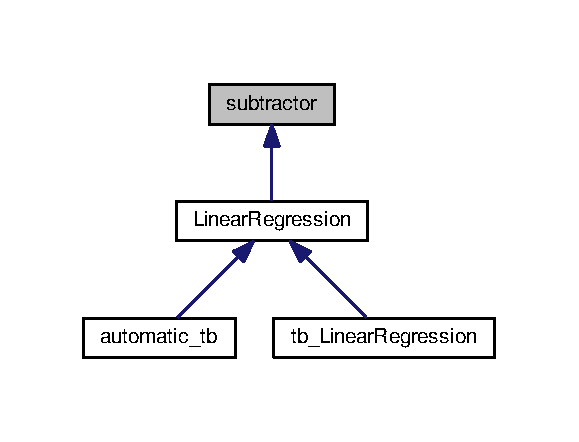
\includegraphics[width=278pt]{classsubtractor__inherit__graph}
\end{center}
\end{figure}
\subsection*{Entities}
\begin{DoxyCompactItemize}
\item 
\hyperlink{classsubtractor_1_1structural}{structural} architecture
\end{DoxyCompactItemize}
\subsection*{Libraries}
 \begin{DoxyCompactItemize}
\item 
\hyperlink{group___subtractor_ga0a6af6eef40212dbaf130d57ce711256}{ieee} 
\end{DoxyCompactItemize}
\subsection*{Use Clauses}
 \begin{DoxyCompactItemize}
\item 
\hyperlink{group___subtractor_gacd03516902501cd1c7296a98e22c6fcb}{std\+\_\+logic\+\_\+1164}   
\item 
\hyperlink{group___subtractor_ga2edc34402b573437d5f25fa90ba4013e}{numeric\+\_\+std}   
\end{DoxyCompactItemize}
\subsection*{Generics}
 \begin{DoxyCompactItemize}
\item 
\hyperlink{group___subtractor_gae1435c07d0cd54b521535e2f8de6f94e}{nbits} {\bfseries {\bfseries \textcolor{vhdlchar}{natural}\textcolor{vhdlchar}{ }\textcolor{vhdlchar}{ }\textcolor{vhdlchar}{\+:}\textcolor{vhdlchar}{=}\textcolor{vhdlchar}{ }\textcolor{vhdlchar}{ } \textcolor{vhdldigit}{32} \textcolor{vhdlchar}{ }}}
\end{DoxyCompactItemize}
\subsection*{Ports}
 \begin{DoxyCompactItemize}
\item 
\hyperlink{group___subtractor_ga49536ce3d87a5522d2d82cc34985d648}{sub1}  {\bfseries {\bfseries \textcolor{vhdlchar}{in}\textcolor{vhdlchar}{ }}} {\bfseries \textcolor{vhdlchar}{std\+\_\+logic\+\_\+vector}\textcolor{vhdlchar}{ }\textcolor{vhdlchar}{(}\textcolor{vhdlchar}{ }\textcolor{vhdlchar}{ }\textcolor{vhdlchar}{ }\textcolor{vhdlchar}{ }{\bfseries \hyperlink{group___subtractor_gae1435c07d0cd54b521535e2f8de6f94e}{nbits}} \textcolor{vhdlchar}{-\/}\textcolor{vhdlchar}{ } \textcolor{vhdldigit}{1} \textcolor{vhdlchar}{ }\textcolor{vhdlchar}{downto}\textcolor{vhdlchar}{ }\textcolor{vhdlchar}{ } \textcolor{vhdldigit}{0} \textcolor{vhdlchar}{ }\textcolor{vhdlchar}{)}\textcolor{vhdlchar}{ }} 
\begin{DoxyCompactList}\small\item\em minuendo \end{DoxyCompactList}\item 
\hyperlink{group___subtractor_ga0c49fa677895a036f45dd76f988d18c5}{sub2}  {\bfseries {\bfseries \textcolor{vhdlchar}{in}\textcolor{vhdlchar}{ }}} {\bfseries \textcolor{vhdlchar}{std\+\_\+logic\+\_\+vector}\textcolor{vhdlchar}{ }\textcolor{vhdlchar}{(}\textcolor{vhdlchar}{ }\textcolor{vhdlchar}{ }\textcolor{vhdlchar}{ }\textcolor{vhdlchar}{ }{\bfseries \hyperlink{group___subtractor_gae1435c07d0cd54b521535e2f8de6f94e}{nbits}} \textcolor{vhdlchar}{-\/}\textcolor{vhdlchar}{ } \textcolor{vhdldigit}{1} \textcolor{vhdlchar}{ }\textcolor{vhdlchar}{downto}\textcolor{vhdlchar}{ }\textcolor{vhdlchar}{ } \textcolor{vhdldigit}{0} \textcolor{vhdlchar}{ }\textcolor{vhdlchar}{)}\textcolor{vhdlchar}{ }} 
\begin{DoxyCompactList}\small\item\em sottraendo \end{DoxyCompactList}\item 
\hyperlink{group___subtractor_ga0fa68103d429fdc11539b6baa81d0d0d}{diff}  {\bfseries {\bfseries \textcolor{vhdlchar}{out}\textcolor{vhdlchar}{ }}} {\bfseries \textcolor{vhdlchar}{std\+\_\+logic\+\_\+vector}\textcolor{vhdlchar}{ }\textcolor{vhdlchar}{(}\textcolor{vhdlchar}{ }\textcolor{vhdlchar}{ }\textcolor{vhdlchar}{ }\textcolor{vhdlchar}{ }{\bfseries \hyperlink{group___subtractor_gae1435c07d0cd54b521535e2f8de6f94e}{nbits}} \textcolor{vhdlchar}{-\/}\textcolor{vhdlchar}{ } \textcolor{vhdldigit}{1} \textcolor{vhdlchar}{ }\textcolor{vhdlchar}{downto}\textcolor{vhdlchar}{ }\textcolor{vhdlchar}{ } \textcolor{vhdldigit}{0} \textcolor{vhdlchar}{ }\textcolor{vhdlchar}{)}\textcolor{vhdlchar}{ }} 
\begin{DoxyCompactList}\small\item\em differenza dei valori\+: diff = sub1-\/sub2 \end{DoxyCompactList}\end{DoxyCompactItemize}


\subsection{Descrizione dettagliata}
Sottrattore di due numeri.

Il sottrattore permette di effettuare una differenza di due numeri espressi su un certo numero di bit. La differenza dei due valori viene espressa sullo stesso numero di bit. 

La documentazione per questa classe è stata generata a partire dal seguente file\+:\begin{DoxyCompactItemize}
\item 
Src/\hyperlink{subtractor_8vhd}{subtractor.\+vhd}\end{DoxyCompactItemize}

\hypertarget{classtb___linear_regression}{}\section{tb\+\_\+\+Linear\+Regression Entity Reference}
\label{classtb___linear_regression}\index{tb\+\_\+\+Linear\+Regression@{tb\+\_\+\+Linear\+Regression}}


Diagramma delle classi per tb\+\_\+\+Linear\+Regression

\chapter{Documentazione dei file}
\hypertarget{_generic_buffer_8vhd}{\section{Riferimenti per il file Src/\+Generic\+Buffer.vhd}
\label{_generic_buffer_8vhd}\index{Src/\+Generic\+Buffer.\+vhd@{Src/\+Generic\+Buffer.\+vhd}}
}
\subsection*{Entities}
\begin{DoxyCompactItemize}
\item 
\hyperlink{class_generic_buffer}{Generic\+Buffer} entity
\begin{DoxyCompactList}\small\item\em Registro di dimensione generica. \end{DoxyCompactList}\item 
\hyperlink{class_generic_buffer_1_1_behavioral}{Behavioral} architecture
\begin{DoxyCompactList}\small\item\em Implementazione behavioral di \hyperlink{class_generic_buffer}{Generic\+Buffer}. \end{DoxyCompactList}\end{DoxyCompactItemize}


\subsection{Descrizione dettagliata}
\begin{DoxyAuthor}{Autore}
Salvatore Barone \href{mailto:salvator.barone@studenti.unina.it}{\tt salvator.\+barone@studenti.\+unina.\+it} Alfonso Di Martino \href{mailto:alf.dimartino@studenti.unina.it}{\tt alf.\+dimartino@studenti.\+unina.\+it} Pietro Liguori \href{mailto:pi.liguori@studenti.unina.it}{\tt pi.\+liguori@studenti.\+unina.\+it} 
\end{DoxyAuthor}
\begin{DoxyDate}{Data}
17-\/04-\/2017
\end{DoxyDate}
Copyright 2017 Salvatore Barone \href{mailto:salvator.barone@gmail.com}{\tt salvator.\+barone@gmail.\+com} ~\newline
 Alfonso Di Martino \href{mailto:alfonsodimartino160989@gmail.com}{\tt alfonsodimartino160989@gmail.\+com} ~\newline
 Pietro Liguori \href{mailto:pie.liguori@gmail.com}{\tt pie.\+liguori@gmail.\+com} ~\newline


This file is part of Linear-\/\+Regression.

Linear-\/\+Regression is free software; you can redistribute it and/or modify it under the terms of the G\+N\+U General Public License as published by the Free Software Foundation; either version 3 of the License, or any later version.

Linear-\/\+Regression is distributed in the hope that it will be useful, but W\+I\+T\+H\+O\+U\+T A\+N\+Y W\+A\+R\+R\+A\+N\+T\+Y; without even the implied warranty of M\+E\+R\+C\+H\+A\+N\+T\+A\+B\+I\+L\+I\+T\+Y or F\+I\+T\+N\+E\+S\+S F\+O\+R A P\+A\+R\+T\+I\+C\+U\+L\+A\+R P\+U\+R\+P\+O\+S\+E. See the G\+N\+U General Public License for more details.

You should have received a copy of the G\+N\+U General Public License along with this program; if not, write to the Free Software Foundation, Inc., 51 Franklin Street, Fifth Floor, Boston, M\+A 02110-\/1301, U\+S\+A. 
\hypertarget{_linear_regression_8vhd}{\section{Riferimenti per il file Src/\+Linear\+Regression.vhd}
\label{_linear_regression_8vhd}\index{Src/\+Linear\+Regression.\+vhd@{Src/\+Linear\+Regression.\+vhd}}
}
\subsection*{Entities}
\begin{DoxyCompactItemize}
\item 
\hyperlink{class_linear_regression}{Linear\+Regression} entity
\item 
\hyperlink{class_linear_regression_1_1_structural}{Structural} architecture
\begin{DoxyCompactList}\small\item\em Per il calcolo dei parametri della regressione vengono utilizzati opportunamente dei moltiplicatori e addizionatori/sottrattori. Per effettuare i calcoli in fixed point vengono adoperati opportuni troncamenti/ espansioni dei segnali. Il componente ha un'architettura pipelined, così come mostrato nello schema di seguito, nel quale sono indicati, usando la notazione standard, le rappresentazioni binarie dei segnali dato in signed fixed-\/point. Si noti che il segnale \char`\"{}load\char`\"{} agisce solo sul primo dei registri della pipe. . \end{DoxyCompactList}\end{DoxyCompactItemize}


\subsection{Descrizione dettagliata}
\begin{DoxyAuthor}{Autori}
Salvatore Barone \href{mailto:salvator.barone@gmail.com}{\tt salvator.\+barone@gmail.\+com} ~\newline
 Alfonso Di Martino \href{mailto:alfonsodimartino160989@gmail.com}{\tt alfonsodimartino160989@gmail.\+com} ~\newline
 Sossio Fiorillo \href{mailto:fsossio@gmail.com}{\tt fsossio@gmail.\+com} ~\newline
 Pietro Liguori \href{mailto:pie.liguori@gmail.com}{\tt pie.\+liguori@gmail.\+com} ~\newline

\end{DoxyAuthor}
\begin{DoxyDate}{Data}
03 07 2017
\end{DoxyDate}
\begin{DoxyCopyright}{Copyright}
Copyright 2017 Salvatore Barone \href{mailto:salvator.barone@gmail.com}{\tt salvator.\+barone@gmail.\+com} ~\newline
 Alfonso Di Martino \href{mailto:alfonsodimartino160989@gmail.com}{\tt alfonsodimartino160989@gmail.\+com} ~\newline
 Sossio Fiorillo \href{mailto:fsossio@gmail.com}{\tt fsossio@gmail.\+com} ~\newline
 Pietro Liguori \href{mailto:pie.liguori@gmail.com}{\tt pie.\+liguori@gmail.\+com} ~\newline

\end{DoxyCopyright}
This file is part of Linear-\/\+Regression.

Linear-\/\+Regression is free software; you can redistribute it and/or modify it under the terms of the G\+N\+U General Public License as published by the Free Software Foundation; either version 3 of the License, or any later version.

Linear-\/\+Regression is distributed in the hope that it will be useful, but W\+I\+T\+H\+O\+U\+T A\+N\+Y W\+A\+R\+R\+A\+N\+T\+Y; without even the implied warranty of M\+E\+R\+C\+H\+A\+N\+T\+A\+B\+I\+L\+I\+T\+Y or F\+I\+T\+N\+E\+S\+S F\+O\+R A P\+A\+R\+T\+I\+C\+U\+L\+A\+R P\+U\+R\+P\+O\+S\+E. See the G\+N\+U General Public License for more details.

You should have received a copy of the G\+N\+U General Public License along with this program; if not, write to the Free Software Foundation, Inc., 51 Franklin Street, Fifth Floor, Boston, M\+A 02110-\/1301, U\+S\+A. 
\hypertarget{multiplier_8vhd}{\section{Riferimenti per il file Src/multiplier.vhd}
\label{multiplier_8vhd}\index{Src/multiplier.\+vhd@{Src/multiplier.\+vhd}}
}
\subsection*{Entities}
\begin{DoxyCompactItemize}
\item 
\hyperlink{classmultiplier}{multiplier} entity
\begin{DoxyCompactList}\small\item\em Moltiplicatore a due fattori. \end{DoxyCompactList}\item 
\hyperlink{classmultiplier_1_1_structural}{Structural} architecture
\begin{DoxyCompactList}\small\item\em Per il prodotto viene utilizzato l'operatore $\ast$. La sintesi viene lasciata al particolare sintetizzatore. \end{DoxyCompactList}\end{DoxyCompactItemize}


\subsection{Descrizione dettagliata}
\begin{DoxyAuthor}{Autori}
Salvatore Barone \href{mailto:salvator.barone@gmail.com}{\tt salvator.\+barone@gmail.\+com} ~\newline
 Alfonso Di Martino \href{mailto:alfonsodimartino160989@gmail.com}{\tt alfonsodimartino160989@gmail.\+com} ~\newline
 Sossio Fiorillo \href{mailto:fsossio@gmail.com}{\tt fsossio@gmail.\+com} ~\newline
 Pietro Liguori \href{mailto:pie.liguori@gmail.com}{\tt pie.\+liguori@gmail.\+com} ~\newline

\end{DoxyAuthor}
\begin{DoxyDate}{Data}
03 07 2017
\end{DoxyDate}
\begin{DoxyCopyright}{Copyright}
Copyright 2017 Salvatore Barone \href{mailto:salvator.barone@gmail.com}{\tt salvator.\+barone@gmail.\+com} ~\newline
 Alfonso Di Martino \href{mailto:alfonsodimartino160989@gmail.com}{\tt alfonsodimartino160989@gmail.\+com} ~\newline
 Sossio Fiorillo \href{mailto:fsossio@gmail.com}{\tt fsossio@gmail.\+com} ~\newline
 Pietro Liguori \href{mailto:pie.liguori@gmail.com}{\tt pie.\+liguori@gmail.\+com} ~\newline

\end{DoxyCopyright}
This file is part of Linear-\/\+Regression.

Linear-\/\+Regression is free software; you can redistribute it and/or modify it under the terms of the G\+N\+U General Public License as published by the Free Software Foundation; either version 3 of the License, or any later version.

Linear-\/\+Regression is distributed in the hope that it will be useful, but W\+I\+T\+H\+O\+U\+T A\+N\+Y W\+A\+R\+R\+A\+N\+T\+Y; without even the implied warranty of M\+E\+R\+C\+H\+A\+N\+T\+A\+B\+I\+L\+I\+T\+Y or F\+I\+T\+N\+E\+S\+S F\+O\+R A P\+A\+R\+T\+I\+C\+U\+L\+A\+R P\+U\+R\+P\+O\+S\+E. See the G\+N\+U General Public License for more details.

You should have received a copy of the G\+N\+U General Public License along with this program; if not, write to the Free Software Foundation, Inc., 51 Franklin Street, Fifth Floor, Boston, M\+A 02110-\/1301, U\+S\+A. 
\hypertarget{subtractor_8vhd}{\section{Riferimenti per il file Src/subtractor.vhd}
\label{subtractor_8vhd}\index{Src/subtractor.\+vhd@{Src/subtractor.\+vhd}}
}
\subsection*{Entities}
\begin{DoxyCompactItemize}
\item 
\hyperlink{classsubtractor}{subtractor} entity
\begin{DoxyCompactList}\small\item\em Sottrattore di due numeri. \end{DoxyCompactList}\item 
\hyperlink{classsubtractor_1_1structural}{structural} architecture
\end{DoxyCompactItemize}


\subsection{Descrizione dettagliata}
\begin{DoxyAuthor}{Autori}
Salvatore Barone \href{mailto:salvator.barone@gmail.com}{\tt salvator.\+barone@gmail.\+com} ~\newline
 Alfonso Di Martino \href{mailto:alfonsodimartino160989@gmail.com}{\tt alfonsodimartino160989@gmail.\+com} ~\newline
 Sossio Fiorillo \href{mailto:fsossio@gmail.com}{\tt fsossio@gmail.\+com} ~\newline
 Pietro Liguori \href{mailto:pie.liguori@gmail.com}{\tt pie.\+liguori@gmail.\+com} ~\newline

\end{DoxyAuthor}
\begin{DoxyDate}{Data}
01 07 2017
\end{DoxyDate}
\begin{DoxyCopyright}{Copyright}
Copyright 2017 Salvatore Barone \href{mailto:salvator.barone@gmail.com}{\tt salvator.\+barone@gmail.\+com} ~\newline
 Alfonso Di Martino \href{mailto:alfonsodimartino160989@gmail.com}{\tt alfonsodimartino160989@gmail.\+com} ~\newline
 Sossio Fiorillo \href{mailto:fsossio@gmail.com}{\tt fsossio@gmail.\+com} ~\newline
 Pietro Liguori \href{mailto:pie.liguori@gmail.com}{\tt pie.\+liguori@gmail.\+com} ~\newline

\end{DoxyCopyright}
This file is part of Linear-\/\+Regression.

Linear-\/\+Regression is free software; you can redistribute it and/or modify it under the terms of the G\+N\+U General Public License as published by the Free Software Foundation; either version 3 of the License, or any later version.

Linear-\/\+Regression is distributed in the hope that it will be useful, but W\+I\+T\+H\+O\+U\+T A\+N\+Y W\+A\+R\+R\+A\+N\+T\+Y; without even the implied warranty of M\+E\+R\+C\+H\+A\+N\+T\+A\+B\+I\+L\+I\+T\+Y or F\+I\+T\+N\+E\+S\+S F\+O\+R A P\+A\+R\+T\+I\+C\+U\+L\+A\+R P\+U\+R\+P\+O\+S\+E. See the G\+N\+U General Public License for more details.

You should have received a copy of the G\+N\+U General Public License along with this program; if not, write to the Free Software Foundation, Inc., 51 Franklin Street, Fifth Floor, Boston, M\+A 02110-\/1301, U\+S\+A. 
\hypertarget{automatic__tb_8vhd}{\section{Riferimenti per il file Src/testbench/automatic\+\_\+tb.vhd}
\label{automatic__tb_8vhd}\index{Src/testbench/automatic\+\_\+tb.\+vhd@{Src/testbench/automatic\+\_\+tb.\+vhd}}
}
\subsection*{Entities}
\begin{DoxyCompactItemize}
\item 
\hyperlink{classautomatic__tb}{automatic\+\_\+tb} entity
\item 
\hyperlink{classautomatic__tb_1_1behavioral}{behavioral} architecture
\end{DoxyCompactItemize}


\subsection{Descrizione dettagliata}
\begin{DoxyAuthor}{Autori}
Salvatore Barone \href{mailto:salvator.barone@gmail.com}{\tt salvator.\+barone@gmail.\+com} ~\newline
 Alfonso Di Martino \href{mailto:alfonsodimartino160989@gmail.com}{\tt alfonsodimartino160989@gmail.\+com} ~\newline
 Sossio Fiorillo \href{mailto:fsossio@gmail.com}{\tt fsossio@gmail.\+com} ~\newline
 Pietro Liguori \href{mailto:pie.liguori@gmail.com}{\tt pie.\+liguori@gmail.\+com} ~\newline

\end{DoxyAuthor}
\begin{DoxyDate}{Data}
05 07 2017
\end{DoxyDate}
\begin{DoxyCopyright}{Copyright}
Copyright 2017 Salvatore Barone \href{mailto:salvator.barone@gmail.com}{\tt salvator.\+barone@gmail.\+com} ~\newline
 Alfonso Di Martino \href{mailto:alfonsodimartino160989@gmail.com}{\tt alfonsodimartino160989@gmail.\+com} ~\newline
 Sossio Fiorillo \href{mailto:fsossio@gmail.com}{\tt fsossio@gmail.\+com} ~\newline
 Pietro Liguori \href{mailto:pie.liguori@gmail.com}{\tt pie.\+liguori@gmail.\+com} ~\newline

\end{DoxyCopyright}
This file is part of Linear-\/\+Regression.

Linear-\/\+Regression is free software; you can redistribute it and/or modify it under the terms of the G\+N\+U General Public License as published by the Free Software Foundation; either version 3 of the License, or any later version.

Linear-\/\+Regression is distributed in the hope that it will be useful, but W\+I\+T\+H\+O\+U\+T A\+N\+Y W\+A\+R\+R\+A\+N\+T\+Y; without even the implied warranty of M\+E\+R\+C\+H\+A\+N\+T\+A\+B\+I\+L\+I\+T\+Y or F\+I\+T\+N\+E\+S\+S F\+O\+R A P\+A\+R\+T\+I\+C\+U\+L\+A\+R P\+U\+R\+P\+O\+S\+E. See the G\+N\+U General Public License for more details.

You should have received a copy of the G\+N\+U General Public License along with this program; if not, write to the Free Software Foundation, Inc., 51 Franklin Street, Fifth Floor, Boston, M\+A 02110-\/1301, U\+S\+A. 
\hypertarget{_calcolo_errore_8m}{}\section{Riferimenti per il file Src/testbench/\+Calcolo\+Errore.m}
\label{_calcolo_errore_8m}\index{Src/testbench/\+Calcolo\+Errore.\+m@{Src/testbench/\+Calcolo\+Errore.\+m}}


\subsection{Documentazione delle funzioni}
\index{Calcolo\+Errore.\+m@{Calcolo\+Errore.\+m}!writetable@{writetable}}
\index{writetable@{writetable}!Calcolo\+Errore.\+m@{Calcolo\+Errore.\+m}}
\subsubsection[{\texorpdfstring{writetable(\+T,\textquotesingle{}error.\+csv\textquotesingle{},\textquotesingle{}\+Write\+Row\+Names\textquotesingle{},true)}{writetable(T,'error.csv','WriteRowNames',true)}}]{\setlength{\rightskip}{0pt plus 5cm}writetable (
\begin{DoxyParamCaption}
\item[{{\bf T}}]{, }
\item[{\textquotesingle{}error.\+csv\textquotesingle{}}]{, }
\item[{\textquotesingle{}Write\+Row\+Names\textquotesingle{}}]{, }
\item[{true}]{}
\end{DoxyParamCaption}
)}\hypertarget{_calcolo_errore_8m_af1c2eb3956d5eceaae8ae64526d80e59}{}\label{_calcolo_errore_8m_af1c2eb3956d5eceaae8ae64526d80e59}


\subsection{Documentazione delle variabili}
\index{Calcolo\+Errore.\+m@{Calcolo\+Errore.\+m}!dataset@{dataset}}
\index{dataset@{dataset}!Calcolo\+Errore.\+m@{Calcolo\+Errore.\+m}}
\subsubsection[{\texorpdfstring{dataset}{dataset}}]{\setlength{\rightskip}{0pt plus 5cm}dataset =textread(\textquotesingle{}dataset.\+txt\textquotesingle{},\textquotesingle{}\%s\textquotesingle{})}\hypertarget{_calcolo_errore_8m_a17a813ff016f566e53dfb54c93ba2913}{}\label{_calcolo_errore_8m_a17a813ff016f566e53dfb54c93ba2913}
\index{Calcolo\+Errore.\+m@{Calcolo\+Errore.\+m}!error\+\_\+m@{error\+\_\+m}}
\index{error\+\_\+m@{error\+\_\+m}!Calcolo\+Errore.\+m@{Calcolo\+Errore.\+m}}
\subsubsection[{\texorpdfstring{error\+\_\+m}{error_m}}]{\setlength{\rightskip}{0pt plus 5cm}error\+\_\+m = abs({\bf m\+\_\+vivado} -\/ {\bf m\+\_\+matlab})}\hypertarget{_calcolo_errore_8m_a27b96081eb8686462fb27b99c9fba619}{}\label{_calcolo_errore_8m_a27b96081eb8686462fb27b99c9fba619}
\index{Calcolo\+Errore.\+m@{Calcolo\+Errore.\+m}!error\+\_\+q@{error\+\_\+q}}
\index{error\+\_\+q@{error\+\_\+q}!Calcolo\+Errore.\+m@{Calcolo\+Errore.\+m}}
\subsubsection[{\texorpdfstring{error\+\_\+q}{error_q}}]{\setlength{\rightskip}{0pt plus 5cm}error\+\_\+q =abs({\bf q\+\_\+vivado}-\/{\bf q\+\_\+matlab})}\hypertarget{_calcolo_errore_8m_a601784e46ab9ea91a638e6ed95b74c0a}{}\label{_calcolo_errore_8m_a601784e46ab9ea91a638e6ed95b74c0a}
\index{Calcolo\+Errore.\+m@{Calcolo\+Errore.\+m}!m\+\_\+matlab@{m\+\_\+matlab}}
\index{m\+\_\+matlab@{m\+\_\+matlab}!Calcolo\+Errore.\+m@{Calcolo\+Errore.\+m}}
\subsubsection[{\texorpdfstring{m\+\_\+matlab}{m_matlab}}]{\setlength{\rightskip}{0pt plus 5cm}m\+\_\+matlab =bin2num(quantizer(\mbox{[}24 13\mbox{]}),{\bf m\+\_\+matlab\+\_\+bin})}\hypertarget{_calcolo_errore_8m_a6280fd49598ab608d04d1614908bd985}{}\label{_calcolo_errore_8m_a6280fd49598ab608d04d1614908bd985}
\index{Calcolo\+Errore.\+m@{Calcolo\+Errore.\+m}!m\+\_\+matlab\+\_\+bin@{m\+\_\+matlab\+\_\+bin}}
\index{m\+\_\+matlab\+\_\+bin@{m\+\_\+matlab\+\_\+bin}!Calcolo\+Errore.\+m@{Calcolo\+Errore.\+m}}
\subsubsection[{\texorpdfstring{m\+\_\+matlab\+\_\+bin}{m_matlab_bin}}]{\setlength{\rightskip}{0pt plus 5cm}m\+\_\+matlab\+\_\+bin = {\bf dataset}(3\+:4\+:end)}\hypertarget{_calcolo_errore_8m_ae36cdc892727b0a3ab1787e3b8911242}{}\label{_calcolo_errore_8m_ae36cdc892727b0a3ab1787e3b8911242}
\index{Calcolo\+Errore.\+m@{Calcolo\+Errore.\+m}!m\+\_\+vivado@{m\+\_\+vivado}}
\index{m\+\_\+vivado@{m\+\_\+vivado}!Calcolo\+Errore.\+m@{Calcolo\+Errore.\+m}}
\subsubsection[{\texorpdfstring{m\+\_\+vivado}{m_vivado}}]{\setlength{\rightskip}{0pt plus 5cm}m\+\_\+vivado =bin2num(quantizer(\mbox{[}24 13\mbox{]}),{\bf m\+\_\+vivado\+\_\+bin})}\hypertarget{_calcolo_errore_8m_a215b43bd10c1abaf6c2058614591f571}{}\label{_calcolo_errore_8m_a215b43bd10c1abaf6c2058614591f571}
\index{Calcolo\+Errore.\+m@{Calcolo\+Errore.\+m}!m\+\_\+vivado\+\_\+bin@{m\+\_\+vivado\+\_\+bin}}
\index{m\+\_\+vivado\+\_\+bin@{m\+\_\+vivado\+\_\+bin}!Calcolo\+Errore.\+m@{Calcolo\+Errore.\+m}}
\subsubsection[{\texorpdfstring{m\+\_\+vivado\+\_\+bin}{m_vivado_bin}}]{\setlength{\rightskip}{0pt plus 5cm}m\+\_\+vivado\+\_\+bin = {\bf out}(1\+:2\+:end)}\hypertarget{_calcolo_errore_8m_a8021bbbc8fbd2af7da73592440faea74}{}\label{_calcolo_errore_8m_a8021bbbc8fbd2af7da73592440faea74}
\index{Calcolo\+Errore.\+m@{Calcolo\+Errore.\+m}!out@{out}}
\index{out@{out}!Calcolo\+Errore.\+m@{Calcolo\+Errore.\+m}}
\subsubsection[{\texorpdfstring{out}{out}}]{\setlength{\rightskip}{0pt plus 5cm}out =textread(\textquotesingle{}output.\+txt\textquotesingle{}, \textquotesingle{}\%s\textquotesingle{})}\hypertarget{_calcolo_errore_8m_a2a89187d8e8e8fba509ef9ab5f815d88}{}\label{_calcolo_errore_8m_a2a89187d8e8e8fba509ef9ab5f815d88}
\index{Calcolo\+Errore.\+m@{Calcolo\+Errore.\+m}!q\+\_\+matlab@{q\+\_\+matlab}}
\index{q\+\_\+matlab@{q\+\_\+matlab}!Calcolo\+Errore.\+m@{Calcolo\+Errore.\+m}}
\subsubsection[{\texorpdfstring{q\+\_\+matlab}{q_matlab}}]{\setlength{\rightskip}{0pt plus 5cm}q\+\_\+matlab =bin2num(quantizer(\mbox{[}24 21\mbox{]}),{\bf q\+\_\+matlab\+\_\+bin})}\hypertarget{_calcolo_errore_8m_ae0ba6f87f318da799b999bc44504e445}{}\label{_calcolo_errore_8m_ae0ba6f87f318da799b999bc44504e445}
\index{Calcolo\+Errore.\+m@{Calcolo\+Errore.\+m}!q\+\_\+matlab\+\_\+bin@{q\+\_\+matlab\+\_\+bin}}
\index{q\+\_\+matlab\+\_\+bin@{q\+\_\+matlab\+\_\+bin}!Calcolo\+Errore.\+m@{Calcolo\+Errore.\+m}}
\subsubsection[{\texorpdfstring{q\+\_\+matlab\+\_\+bin}{q_matlab_bin}}]{\setlength{\rightskip}{0pt plus 5cm}q\+\_\+matlab\+\_\+bin = {\bf dataset}(4\+:4\+:end)}\hypertarget{_calcolo_errore_8m_af2824fe5b103500c8f44114732ab01e6}{}\label{_calcolo_errore_8m_af2824fe5b103500c8f44114732ab01e6}
\index{Calcolo\+Errore.\+m@{Calcolo\+Errore.\+m}!q\+\_\+vivado@{q\+\_\+vivado}}
\index{q\+\_\+vivado@{q\+\_\+vivado}!Calcolo\+Errore.\+m@{Calcolo\+Errore.\+m}}
\subsubsection[{\texorpdfstring{q\+\_\+vivado}{q_vivado}}]{\setlength{\rightskip}{0pt plus 5cm}q\+\_\+vivado =bin2num(quantizer(\mbox{[}24 21\mbox{]}),{\bf q\+\_\+vivado\+\_\+bin})}\hypertarget{_calcolo_errore_8m_aef958b87ed02ad2a876d2e5160ed0650}{}\label{_calcolo_errore_8m_aef958b87ed02ad2a876d2e5160ed0650}
\index{Calcolo\+Errore.\+m@{Calcolo\+Errore.\+m}!q\+\_\+vivado\+\_\+bin@{q\+\_\+vivado\+\_\+bin}}
\index{q\+\_\+vivado\+\_\+bin@{q\+\_\+vivado\+\_\+bin}!Calcolo\+Errore.\+m@{Calcolo\+Errore.\+m}}
\subsubsection[{\texorpdfstring{q\+\_\+vivado\+\_\+bin}{q_vivado_bin}}]{\setlength{\rightskip}{0pt plus 5cm}q\+\_\+vivado\+\_\+bin = {\bf out}(2\+:2\+:end)}\hypertarget{_calcolo_errore_8m_a86c185cb9619b1646488d659e5bc4648}{}\label{_calcolo_errore_8m_a86c185cb9619b1646488d659e5bc4648}
\index{Calcolo\+Errore.\+m@{Calcolo\+Errore.\+m}!T@{T}}
\index{T@{T}!Calcolo\+Errore.\+m@{Calcolo\+Errore.\+m}}
\subsubsection[{\texorpdfstring{T}{T}}]{\setlength{\rightskip}{0pt plus 5cm}T = table({\bf m\+\_\+matlab}, {\bf q\+\_\+matlab},{\bf m\+\_\+vivado},{\bf q\+\_\+vivado}, {\bf error\+\_\+m}, {\bf error\+\_\+q})}\hypertarget{_calcolo_errore_8m_adf1f3edb9115acb0a1e04209b7a9937b}{}\label{_calcolo_errore_8m_adf1f3edb9115acb0a1e04209b7a9937b}

\hypertarget{tb___linear_regression_8vhd}{}\section{Riferimenti per il file Src/tb\+\_\+\+Linear\+Regression.vhd}
\label{tb___linear_regression_8vhd}\index{Src/tb\+\_\+\+Linear\+Regression.\+vhd@{Src/tb\+\_\+\+Linear\+Regression.\+vhd}}
\subsection*{Entities}
\begin{DoxyCompactItemize}
\item 
\hyperlink{classtb___linear_regression}{tb\+\_\+\+Linear\+Regression} entity
\item 
\hyperlink{classtb___linear_regression_1_1_behavioral}{Behavioral} architecture
\end{DoxyCompactItemize}


\subsection{Descrizione dettagliata}
\begin{DoxyAuthor}{Autori}
Salvatore Barone \href{mailto:salvator.barone@gmail.com}{\tt salvator.\+barone@gmail.\+com} ~\newline
 Alfonso Di Martino \href{mailto:alfonsodimartino160989@gmail.com}{\tt alfonsodimartino160989@gmail.\+com} ~\newline
 Sossio Fiorillo \href{mailto:fsossio@gmail.com}{\tt fsossio@gmail.\+com} ~\newline
 Pietro Liguori \href{mailto:pie.liguori@gmail.com}{\tt pie.\+liguori@gmail.\+com} ~\newline

\end{DoxyAuthor}
\begin{DoxyDate}{Data}
03 07 2017
\end{DoxyDate}
\begin{DoxyCopyright}{Copyright}
Copyright 2017 Salvatore Barone \href{mailto:salvator.barone@gmail.com}{\tt salvator.\+barone@gmail.\+com} ~\newline
 Alfonso Di Martino \href{mailto:alfonsodimartino160989@gmail.com}{\tt alfonsodimartino160989@gmail.\+com} ~\newline
 Sossio Fiorillo \href{mailto:fsossio@gmail.com}{\tt fsossio@gmail.\+com} ~\newline
 Pietro Liguori \href{mailto:pie.liguori@gmail.com}{\tt pie.\+liguori@gmail.\+com} ~\newline

\end{DoxyCopyright}
This file is part of Linear-\/\+Regression.

Linear-\/\+Regression is free software; you can redistribute it and/or modify it under the terms of the G\+NU General Public License as published by the Free Software Foundation; either version 3 of the License, or any later version.

Linear-\/\+Regression is distributed in the hope that it will be useful, but W\+I\+T\+H\+O\+UT A\+NY W\+A\+R\+R\+A\+N\+TY; without even the implied warranty of M\+E\+R\+C\+H\+A\+N\+T\+A\+B\+I\+L\+I\+TY or F\+I\+T\+N\+E\+SS F\+OR A P\+A\+R\+T\+I\+C\+U\+L\+AR P\+U\+R\+P\+O\+SE. See the G\+NU General Public License for more details.

You should have received a copy of the G\+NU General Public License along with this program; if not, write to the Free Software Foundation, Inc., 51 Franklin Street, Fifth Floor, Boston, MA 02110-\/1301, U\+SA. 
\hypertarget{_t_bgenerator_8m}{}\section{Riferimenti per il file Src/testbench/\+T\+Bgenerator.m}
\label{_t_bgenerator_8m}\index{Src/testbench/\+T\+Bgenerator.\+m@{Src/testbench/\+T\+Bgenerator.\+m}}


\subsection{Documentazione delle funzioni}
\index{T\+Bgenerator.\+m@{T\+Bgenerator.\+m}!code@{code}}
\index{code@{code}!T\+Bgenerator.\+m@{T\+Bgenerator.\+m}}
\subsubsection[{\texorpdfstring{code(s) x}{code(s) x}}]{\setlength{\rightskip}{0pt plus 5cm}Length of primary code (
\begin{DoxyParamCaption}
\item[{s}]{}
\end{DoxyParamCaption}
)}\hypertarget{_t_bgenerator_8m_a22dc5d063516961eac6a2b32173c1e9d}{}\label{_t_bgenerator_8m_a22dc5d063516961eac6a2b32173c1e9d}
\index{T\+Bgenerator.\+m@{T\+Bgenerator.\+m}!fclose@{fclose}}
\index{fclose@{fclose}!T\+Bgenerator.\+m@{T\+Bgenerator.\+m}}
\subsubsection[{\texorpdfstring{fclose(fid)}{fclose(fid)}}]{\setlength{\rightskip}{0pt plus 5cm}Remember to add r {\bf n} to end lines ! end fclose (
\begin{DoxyParamCaption}
\item[{{\bf fid}}]{}
\end{DoxyParamCaption}
)}\hypertarget{_t_bgenerator_8m_a15ae9884c702ae433284a239587f3731}{}\label{_t_bgenerator_8m_a15ae9884c702ae433284a239587f3731}
\index{T\+Bgenerator.\+m@{T\+Bgenerator.\+m}!frequency@{frequency}}
\index{frequency@{frequency}!T\+Bgenerator.\+m@{T\+Bgenerator.\+m}}
\subsubsection[{\texorpdfstring{frequency(\+Hz) dt}{frequency(Hz) dt}}]{\setlength{\rightskip}{0pt plus 5cm}Sampling frequency (
\begin{DoxyParamCaption}
\item[{Hz}]{}
\end{DoxyParamCaption}
)}\hypertarget{_t_bgenerator_8m_ab4937012ababa663c64f02b829612907}{}\label{_t_bgenerator_8m_ab4937012ababa663c64f02b829612907}
\index{T\+Bgenerator.\+m@{T\+Bgenerator.\+m}!fwrite@{fwrite}}
\index{fwrite@{fwrite}!T\+Bgenerator.\+m@{T\+Bgenerator.\+m}}
\subsubsection[{\texorpdfstring{fwrite(fid,[s1\+\_\+bin char(32) s2\+\_\+bin char(32) m\+\_\+bin char(32) q\+\_\+bin char(32) char(13) char(10)])}{fwrite(fid,[s1_bin char(32) s2_bin char(32) m_bin char(32) q_bin char(32) char(13) char(10)])}}]{\setlength{\rightskip}{0pt plus 5cm}fwrite (
\begin{DoxyParamCaption}
\item[{{\bf fid}}]{}
\end{DoxyParamCaption}
)}\hypertarget{_t_bgenerator_8m_a23abf1104e243a25ff9ee8d924268304}{}\label{_t_bgenerator_8m_a23abf1104e243a25ff9ee8d924268304}
\index{T\+Bgenerator.\+m@{T\+Bgenerator.\+m}!m@{m}}
\index{m@{m}!T\+Bgenerator.\+m@{T\+Bgenerator.\+m}}
\subsubsection[{\texorpdfstring{m(j,1) }{m(j,1) }}]{\setlength{\rightskip}{0pt plus 5cm}m (
\begin{DoxyParamCaption}
\item[{{\bf j}}]{, }
\item[{1}]{}
\end{DoxyParamCaption}
)}\hypertarget{_t_bgenerator_8m_aa8e6e0e3cdb6469cd5aeff39b94135c6}{}\label{_t_bgenerator_8m_aa8e6e0e3cdb6469cd5aeff39b94135c6}
\index{T\+Bgenerator.\+m@{T\+Bgenerator.\+m}!mult1@{mult1}}
\index{mult1@{mult1}!T\+Bgenerator.\+m@{T\+Bgenerator.\+m}}
\subsubsection[{\texorpdfstring{mult1(j,1)}{mult1(j,1)}}]{\setlength{\rightskip}{0pt plus 5cm}mult1 (
\begin{DoxyParamCaption}
\item[{{\bf j}}]{, }
\item[{1}]{}
\end{DoxyParamCaption}
)}\hypertarget{_t_bgenerator_8m_aa797aa9d4fbea894dfdbf23086369ed3}{}\label{_t_bgenerator_8m_aa797aa9d4fbea894dfdbf23086369ed3}
\index{T\+Bgenerator.\+m@{T\+Bgenerator.\+m}!mult2@{mult2}}
\index{mult2@{mult2}!T\+Bgenerator.\+m@{T\+Bgenerator.\+m}}
\subsubsection[{\texorpdfstring{mult2(j,1)}{mult2(j,1)}}]{\setlength{\rightskip}{0pt plus 5cm}mult2 (
\begin{DoxyParamCaption}
\item[{{\bf j}}]{, }
\item[{1}]{}
\end{DoxyParamCaption}
)}\hypertarget{_t_bgenerator_8m_a0e083f3ee29ce5827eeab161669b163e}{}\label{_t_bgenerator_8m_a0e083f3ee29ce5827eeab161669b163e}
\index{T\+Bgenerator.\+m@{T\+Bgenerator.\+m}!mult3@{mult3}}
\index{mult3@{mult3}!T\+Bgenerator.\+m@{T\+Bgenerator.\+m}}
\subsubsection[{\texorpdfstring{mult3(j,1)}{mult3(j,1)}}]{\setlength{\rightskip}{0pt plus 5cm}mult3 (
\begin{DoxyParamCaption}
\item[{{\bf j}}]{, }
\item[{1}]{}
\end{DoxyParamCaption}
)}\hypertarget{_t_bgenerator_8m_acedd0c47e7f6f3c5238dac540150c7ec}{}\label{_t_bgenerator_8m_acedd0c47e7f6f3c5238dac540150c7ec}
\index{T\+Bgenerator.\+m@{T\+Bgenerator.\+m}!mult4@{mult4}}
\index{mult4@{mult4}!T\+Bgenerator.\+m@{T\+Bgenerator.\+m}}
\subsubsection[{\texorpdfstring{mult4(j,1)}{mult4(j,1)}}]{\setlength{\rightskip}{0pt plus 5cm}mult4 (
\begin{DoxyParamCaption}
\item[{{\bf j}}]{, }
\item[{1}]{}
\end{DoxyParamCaption}
)}\hypertarget{_t_bgenerator_8m_a02e514c5873302cdb7cf04cb9e65a13e}{}\label{_t_bgenerator_8m_a02e514c5873302cdb7cf04cb9e65a13e}
\index{T\+Bgenerator.\+m@{T\+Bgenerator.\+m}!points@{points}}
\index{points@{points}!T\+Bgenerator.\+m@{T\+Bgenerator.\+m}}
\subsubsection[{\texorpdfstring{points(s) t\+\_\+fast }{points(s) t_fast }}]{\setlength{\rightskip}{0pt plus 5cm}Time distance between points (
\begin{DoxyParamCaption}
\item[{s}]{}
\end{DoxyParamCaption}
)}\hypertarget{_t_bgenerator_8m_af6238d69bf69bc1ac7e32e239eab32c2}{}\label{_t_bgenerator_8m_af6238d69bf69bc1ac7e32e239eab32c2}
\index{T\+Bgenerator.\+m@{T\+Bgenerator.\+m}!q@{q}}
\index{q@{q}!T\+Bgenerator.\+m@{T\+Bgenerator.\+m}}
\subsubsection[{\texorpdfstring{q(j,1)}{q(j,1)}}]{\setlength{\rightskip}{0pt plus 5cm}q (
\begin{DoxyParamCaption}
\item[{{\bf j}}]{, }
\item[{1}]{}
\end{DoxyParamCaption}
)}\hypertarget{_t_bgenerator_8m_a6c9ce0820dfce3e4f3b8bb481989ba8d}{}\label{_t_bgenerator_8m_a6c9ce0820dfce3e4f3b8bb481989ba8d}
\index{T\+Bgenerator.\+m@{T\+Bgenerator.\+m}!sig@{sig}}
\index{sig@{sig}!T\+Bgenerator.\+m@{T\+Bgenerator.\+m}}
\subsubsection[{\texorpdfstring{sig(1)}{sig(1)}}]{\setlength{\rightskip}{0pt plus 5cm}sig (
\begin{DoxyParamCaption}
\item[{1}]{}
\end{DoxyParamCaption}
)}\hypertarget{_t_bgenerator_8m_ad2d78cd5d260044b4279194fa2519512}{}\label{_t_bgenerator_8m_ad2d78cd5d260044b4279194fa2519512}
\index{T\+Bgenerator.\+m@{T\+Bgenerator.\+m}!step@{step}}
\index{step@{step}!T\+Bgenerator.\+m@{T\+Bgenerator.\+m}}
\subsubsection[{\texorpdfstring{step(s) T\+\_\+\+P = 0.\+001}{step(s) T_P = 0.001}}]{\setlength{\rightskip}{0pt plus 5cm}Time step (
\begin{DoxyParamCaption}
\item[{s}]{}
\end{DoxyParamCaption}
)\hspace{0.3cm}{\ttfamily [pure virtual]}}\hypertarget{_t_bgenerator_8m_a7c499df78f2a324879ac63e167130016}{}\label{_t_bgenerator_8m_a7c499df78f2a324879ac63e167130016}
\index{T\+Bgenerator.\+m@{T\+Bgenerator.\+m}!sub5@{sub5}}
\index{sub5@{sub5}!T\+Bgenerator.\+m@{T\+Bgenerator.\+m}}
\subsubsection[{\texorpdfstring{sub5(j,1)}{sub5(j,1)}}]{\setlength{\rightskip}{0pt plus 5cm}sub5 (
\begin{DoxyParamCaption}
\item[{{\bf j}}]{, }
\item[{1}]{}
\end{DoxyParamCaption}
)}\hypertarget{_t_bgenerator_8m_a3d9688f40693448a2669ac50321cc62f}{}\label{_t_bgenerator_8m_a3d9688f40693448a2669ac50321cc62f}
\index{T\+Bgenerator.\+m@{T\+Bgenerator.\+m}!sub6@{sub6}}
\index{sub6@{sub6}!T\+Bgenerator.\+m@{T\+Bgenerator.\+m}}
\subsubsection[{\texorpdfstring{sub6(j,1)}{sub6(j,1)}}]{\setlength{\rightskip}{0pt plus 5cm}sub6 (
\begin{DoxyParamCaption}
\item[{{\bf j}}]{, }
\item[{1}]{}
\end{DoxyParamCaption}
)}\hypertarget{_t_bgenerator_8m_adc3576c1d4f5400868680a458addd07f}{}\label{_t_bgenerator_8m_adc3576c1d4f5400868680a458addd07f}
\index{T\+Bgenerator.\+m@{T\+Bgenerator.\+m}!sum1@{sum1}}
\index{sum1@{sum1}!T\+Bgenerator.\+m@{T\+Bgenerator.\+m}}
\subsubsection[{\texorpdfstring{sum1(j,1)}{sum1(j,1)}}]{\setlength{\rightskip}{0pt plus 5cm}sum1 (
\begin{DoxyParamCaption}
\item[{{\bf j}}]{, }
\item[{1}]{}
\end{DoxyParamCaption}
)}\hypertarget{_t_bgenerator_8m_aee1c9f386ada5225ab3335a19ff4284a}{}\label{_t_bgenerator_8m_aee1c9f386ada5225ab3335a19ff4284a}
\index{T\+Bgenerator.\+m@{T\+Bgenerator.\+m}!sum2@{sum2}}
\index{sum2@{sum2}!T\+Bgenerator.\+m@{T\+Bgenerator.\+m}}
\subsubsection[{\texorpdfstring{sum2(j,1)}{sum2(j,1)}}]{\setlength{\rightskip}{0pt plus 5cm}sum2 (
\begin{DoxyParamCaption}
\item[{{\bf j}}]{, }
\item[{1}]{}
\end{DoxyParamCaption}
)}\hypertarget{_t_bgenerator_8m_a5479064783cea1e00d7ee9fcfed41ca0}{}\label{_t_bgenerator_8m_a5479064783cea1e00d7ee9fcfed41ca0}


\subsection{Documentazione delle variabili}
\index{T\+Bgenerator.\+m@{T\+Bgenerator.\+m}!div1@{div1}}
\index{div1@{div1}!T\+Bgenerator.\+m@{T\+Bgenerator.\+m}}
\subsubsection[{\texorpdfstring{div1}{div1}}]{\setlength{\rightskip}{0pt plus 5cm}div1 =1/(({\bf n}$\ast${\bf sx2})-\/{\bf s2x})}\hypertarget{_t_bgenerator_8m_a6242f4aca888b19ebb89fb0389ecdaa2}{}\label{_t_bgenerator_8m_a6242f4aca888b19ebb89fb0389ecdaa2}
\index{T\+Bgenerator.\+m@{T\+Bgenerator.\+m}!fid@{fid}}
\index{fid@{fid}!T\+Bgenerator.\+m@{T\+Bgenerator.\+m}}
\subsubsection[{\texorpdfstring{fid}{fid}}]{\setlength{\rightskip}{0pt plus 5cm}Filename fid = fopen({\bf my\+File},\textquotesingle{}w\textquotesingle{})}\hypertarget{_t_bgenerator_8m_a0937ca518a49a43daf9762012eeaed03}{}\label{_t_bgenerator_8m_a0937ca518a49a43daf9762012eeaed03}
\index{T\+Bgenerator.\+m@{T\+Bgenerator.\+m}!fs@{fs}}
\index{fs@{fs}!T\+Bgenerator.\+m@{T\+Bgenerator.\+m}}
\subsubsection[{\texorpdfstring{fs}{fs}}]{\setlength{\rightskip}{0pt plus 5cm}Number of elements for test fs =20460000}\hypertarget{_t_bgenerator_8m_ac1ba0666dde046157a6a499ea03fd56c}{}\label{_t_bgenerator_8m_ac1ba0666dde046157a6a499ea03fd56c}
\index{T\+Bgenerator.\+m@{T\+Bgenerator.\+m}!i@{i}}
\index{i@{i}!T\+Bgenerator.\+m@{T\+Bgenerator.\+m}}
\subsubsection[{\texorpdfstring{i}{i}}]{\setlength{\rightskip}{0pt plus 5cm}This signal simulates the output of an atan2 module for i}\hypertarget{_t_bgenerator_8m_aac0842b0a34028f5ea3b578a1e662414}{}\label{_t_bgenerator_8m_aac0842b0a34028f5ea3b578a1e662414}
{\bfseries Valore iniziale\+:}
\begin{DoxyCode}
=2:length(\hyperlink{_t_bgenerator_8m_a6dcde76e9e1818a146ac3de6b51798a5}{sig})
        \hyperlink{_t_bgenerator_8m_a6dcde76e9e1818a146ac3de6b51798a5}{sig}(\hyperlink{_t_bgenerator_8m_aac0842b0a34028f5ea3b578a1e662414}{i})=\hyperlink{_t_bgenerator_8m_a6dcde76e9e1818a146ac3de6b51798a5}{sig}(\hyperlink{_t_bgenerator_8m_aac0842b0a34028f5ea3b578a1e662414}{i}-1)+rand()-0.2
\end{DoxyCode}
\index{T\+Bgenerator.\+m@{T\+Bgenerator.\+m}!j@{j}}
\index{j@{j}!T\+Bgenerator.\+m@{T\+Bgenerator.\+m}}
\subsubsection[{\texorpdfstring{j}{j}}]{\setlength{\rightskip}{0pt plus 5cm}Open file for j}\hypertarget{_t_bgenerator_8m_a2965c10e4c6f4f2a86db0ae1e7126506}{}\label{_t_bgenerator_8m_a2965c10e4c6f4f2a86db0ae1e7126506}
{\bfseries Valore iniziale\+:}
\begin{DoxyCode}
=1:10000
    
    \hyperlink{_t_bgenerator_8m_a6dcde76e9e1818a146ac3de6b51798a5}{sig}=zeros(1,\hyperlink{_t_bgenerator_8m_aeab71244afb687f16d8c4f5ee9d6ef0e}{n})
\end{DoxyCode}
\index{T\+Bgenerator.\+m@{T\+Bgenerator.\+m}!m@{m}}
\index{m@{m}!T\+Bgenerator.\+m@{T\+Bgenerator.\+m}}
\subsubsection[{\texorpdfstring{m}{m}}]{\setlength{\rightskip}{0pt plus 5cm}m = ({\bf n}$\ast${\bf s2} -\/ {\bf s1}$\ast$sx) $\ast${\bf div1}}\hypertarget{_t_bgenerator_8m_ab3cd915d758008bd19d0f2428fbb354a}{}\label{_t_bgenerator_8m_ab3cd915d758008bd19d0f2428fbb354a}
\index{T\+Bgenerator.\+m@{T\+Bgenerator.\+m}!m\+\_\+bin@{m\+\_\+bin}}
\index{m\+\_\+bin@{m\+\_\+bin}!T\+Bgenerator.\+m@{T\+Bgenerator.\+m}}
\subsubsection[{\texorpdfstring{m\+\_\+bin}{m_bin}}]{\setlength{\rightskip}{0pt plus 5cm}m\+\_\+bin = num2bin(quantizer(\mbox{[}24 13\mbox{]}),{\bf m})}\hypertarget{_t_bgenerator_8m_a4a8ff9ce1772854d4d02a78e413cd143}{}\label{_t_bgenerator_8m_a4a8ff9ce1772854d4d02a78e413cd143}
\index{T\+Bgenerator.\+m@{T\+Bgenerator.\+m}!my\+File@{my\+File}}
\index{my\+File@{my\+File}!T\+Bgenerator.\+m@{T\+Bgenerator.\+m}}
\subsubsection[{\texorpdfstring{my\+File}{myFile}}]{\setlength{\rightskip}{0pt plus 5cm}fast time axis \mbox{[}s\mbox{]} my\+File =\textquotesingle{}dataset.\+txt\textquotesingle{}}\hypertarget{_t_bgenerator_8m_a5f21c46eb6d68dd74e5b316c221f865f}{}\label{_t_bgenerator_8m_a5f21c46eb6d68dd74e5b316c221f865f}
\index{T\+Bgenerator.\+m@{T\+Bgenerator.\+m}!n@{n}}
\index{n@{n}!T\+Bgenerator.\+m@{T\+Bgenerator.\+m}}
\subsubsection[{\texorpdfstring{n}{n}}]{\setlength{\rightskip}{0pt plus 5cm}n =25}\hypertarget{_t_bgenerator_8m_aeab71244afb687f16d8c4f5ee9d6ef0e}{}\label{_t_bgenerator_8m_aeab71244afb687f16d8c4f5ee9d6ef0e}
\index{T\+Bgenerator.\+m@{T\+Bgenerator.\+m}!q@{q}}
\index{q@{q}!T\+Bgenerator.\+m@{T\+Bgenerator.\+m}}
\subsubsection[{\texorpdfstring{q}{q}}]{\setlength{\rightskip}{0pt plus 5cm}q = ({\bf s1}$\ast${\bf sx2} -\/ sx$\ast${\bf s2}) $\ast${\bf div1}}\hypertarget{_t_bgenerator_8m_a099b3b060154898840f0ebdfb46ec78f}{}\label{_t_bgenerator_8m_a099b3b060154898840f0ebdfb46ec78f}
\index{T\+Bgenerator.\+m@{T\+Bgenerator.\+m}!q\+\_\+bin@{q\+\_\+bin}}
\index{q\+\_\+bin@{q\+\_\+bin}!T\+Bgenerator.\+m@{T\+Bgenerator.\+m}}
\subsubsection[{\texorpdfstring{q\+\_\+bin}{q_bin}}]{\setlength{\rightskip}{0pt plus 5cm}q\+\_\+bin = num2bin(quantizer(\mbox{[}24 21\mbox{]}),{\bf q})}\hypertarget{_t_bgenerator_8m_a1109e82811bf1af80a5dedd87c3f3ffc}{}\label{_t_bgenerator_8m_a1109e82811bf1af80a5dedd87c3f3ffc}
\index{T\+Bgenerator.\+m@{T\+Bgenerator.\+m}!s1@{s1}}
\index{s1@{s1}!T\+Bgenerator.\+m@{T\+Bgenerator.\+m}}
\subsubsection[{\texorpdfstring{s1}{s1}}]{\setlength{\rightskip}{0pt plus 5cm}Compute operations s1 =sum({\bf sig})}\hypertarget{_t_bgenerator_8m_a8c3c564326dcc104016fa23b00c20dc9}{}\label{_t_bgenerator_8m_a8c3c564326dcc104016fa23b00c20dc9}
\index{T\+Bgenerator.\+m@{T\+Bgenerator.\+m}!s1\+\_\+bin@{s1\+\_\+bin}}
\index{s1\+\_\+bin@{s1\+\_\+bin}!T\+Bgenerator.\+m@{T\+Bgenerator.\+m}}
\subsubsection[{\texorpdfstring{s1\+\_\+bin}{s1_bin}}]{\setlength{\rightskip}{0pt plus 5cm}Write data on file s1\+\_\+bin = num2bin(quantizer(\mbox{[}24 15\mbox{]}),{\bf s1})}\hypertarget{_t_bgenerator_8m_a42b4b41e1290e8c14bce6943d13fcc35}{}\label{_t_bgenerator_8m_a42b4b41e1290e8c14bce6943d13fcc35}
\index{T\+Bgenerator.\+m@{T\+Bgenerator.\+m}!s2@{s2}}
\index{s2@{s2}!T\+Bgenerator.\+m@{T\+Bgenerator.\+m}}
\subsubsection[{\texorpdfstring{s2}{s2}}]{\setlength{\rightskip}{0pt plus 5cm}s2 =sum(x.$\ast${\bf sig})}\hypertarget{_t_bgenerator_8m_a2e63e71737e8b6802b81f6a7c5ca6a0a}{}\label{_t_bgenerator_8m_a2e63e71737e8b6802b81f6a7c5ca6a0a}
\index{T\+Bgenerator.\+m@{T\+Bgenerator.\+m}!s2\+\_\+bin@{s2\+\_\+bin}}
\index{s2\+\_\+bin@{s2\+\_\+bin}!T\+Bgenerator.\+m@{T\+Bgenerator.\+m}}
\subsubsection[{\texorpdfstring{s2\+\_\+bin}{s2_bin}}]{\setlength{\rightskip}{0pt plus 5cm}Generate binary string s2\+\_\+bin = num2bin(quantizer(\mbox{[}24 21\mbox{]}),{\bf s2})}\hypertarget{_t_bgenerator_8m_a510e1bfbb2e3c7225169b38a5a23018a}{}\label{_t_bgenerator_8m_a510e1bfbb2e3c7225169b38a5a23018a}
\index{T\+Bgenerator.\+m@{T\+Bgenerator.\+m}!s2x@{s2x}}
\index{s2x@{s2x}!T\+Bgenerator.\+m@{T\+Bgenerator.\+m}}
\subsubsection[{\texorpdfstring{s2x}{s2x}}]{\setlength{\rightskip}{0pt plus 5cm}s2x =(sum(x)).$^\wedge$2}\hypertarget{_t_bgenerator_8m_a783d22f774560399ae30f5b7c3402625}{}\label{_t_bgenerator_8m_a783d22f774560399ae30f5b7c3402625}
\index{T\+Bgenerator.\+m@{T\+Bgenerator.\+m}!sig@{sig}}
\index{sig@{sig}!T\+Bgenerator.\+m@{T\+Bgenerator.\+m}}
\subsubsection[{\texorpdfstring{sig}{sig}}]{\setlength{\rightskip}{0pt plus 5cm}end sig =unwrap(sig)}\hypertarget{_t_bgenerator_8m_a6dcde76e9e1818a146ac3de6b51798a5}{}\label{_t_bgenerator_8m_a6dcde76e9e1818a146ac3de6b51798a5}
\index{T\+Bgenerator.\+m@{T\+Bgenerator.\+m}!sx2@{sx2}}
\index{sx2@{sx2}!T\+Bgenerator.\+m@{T\+Bgenerator.\+m}}
\subsubsection[{\texorpdfstring{sx2}{sx2}}]{\setlength{\rightskip}{0pt plus 5cm}sx2 =sum(x.$^\wedge$2)}\hypertarget{_t_bgenerator_8m_a1b65f061f4c6b0f23e32a9489abb8c43}{}\label{_t_bgenerator_8m_a1b65f061f4c6b0f23e32a9489abb8c43}

%--- End generated contents ---

% Index
\newpage
\phantomsection
\addcontentsline{toc}{chapter}{Indice}
\printindex

\end{document}
